%% ----------------ATENCIÓ-----------------------
%% Aquest document està preparat per codificació 
%% UTF-8. Si es llegeix amb un editor 
%% preparat per una altra codificació alguns 
%% caràcters no es veuran correctament.
%%---------------------------------------------- 
%%
%% Aquest document vos pot servir de base per la
%% realització de la memòria del treball final de
%% grau. Es recomana seguir els consells que 
%% apareixen en els diferents comentaris del 
%% document. Convindrà mantenir l'estructura
%% d'aquest exemple i introduir canvis sols 
%% allà on s'indiqui.
%%
%%-----------------------------------------------
%%
%% La plantilla preparada per a la realització de
%% la memòria és la classe LaTeX TFGEPSUIB.cls
%% que es fonamenta en la classe memoir. Aquesta
%% emula alguns `packages` que, per tant, no serà
%% necessari incloure dins el vostre document. El
%% manual de memoir explica quins són aquests
%% paquets (per exemple booktabs, array, tabluarx). 
%% Per altra banda, TFGEPSUIB també carrega 
%% automàticament els paquets, fontenc, xcolor, 
%% graphicx i microtype.
%%
%%-----------------------------------------
%% Opcions de la classe TFGEPSUIB:
%%
%% Per defecte, la classe TFGEPSUIB suposa
%% que la memòria es redactarà en català i que 
%% els estudis són els de Grau en Enginyeria
%% telemàtica. 
%%
%% Si preferiu utilitzar el castellà o anglés
%% per a la redacció de la memòria podeu
%% fer-ho indicant-ho a les opcions.
%\documentclass[catalan]{TFGEPSUIB}
\documentclass[spanish,GINF]{TFGEPSUIB}
%%
%% Per indicar quins són els estudis pels quals
%% es redacta la memòria heu d'incloure una de
%% les següents opcions:
%%
%% GTEL - Grau en Enginyeria Telemàtica
%% GMAT - Grau de Matemàtiques
%% GINF - Grau d'Enginyeria Informàtica
%% GEDI - Grau d'Enginyeria d'Edificació
%% GELE - Grau d'Eng. Elec. Ind. i Automàtica
%% GAGR - Grau en Eng. Agroali. i del Medi Rural
%%
%% Per escriure la memòria en castellà pels estudis
%% de matemàtiques, la línia inicial serà
%\documentclass[spanish,GMAT]{TFGEPSUIB}
%%------------------------------------------

% Per incloure expressions matemàtiques en
% el document és recomanable usar els paquets
%\usepackage{amsmath,mathtools} 

% Per incloure fragments de codi hi ha diferents
% paquets disponibles. Triau el que vos sigui 
% més convenient, per exemple listings. 
%\usepackage{listings} 

% Amb tcolorbox podeu definir caixes per llistats,
% teoremes, exemples, ...
%\usepackage{tcolorbox}

% Si voleu que les referències bibliogràfiques
% apareguin amb el format "autor-any" en comptes 
% de "número" heu d'usar el paquet natbib.
%\usepackage[round,colon,sort&compress]{natbib} 

% En general, la documentació tècnica pot
% incloure molts acrònims. Per això es recomana
% usar el següent paquet. Consultau el corresponent
% manual per saber com s'usa.
\usepackage[printonlyused]{acronym}

% Les diferents unitats de mesura tenen un
% format estàndard de representació que convé
% respectar. Per això s'usa el paquet `siunitx`.
% També permet representar nombres en notació
% científica i alinear correctament els valors 
% numèrics a les taules. Pegau una ullada al 
% manual. Si no voleu usar-lo comentau la línia. 
\usepackage{siunitx}

% Com que és convenient que el paquet hyperref
% sigui un dels darrers en carregar-se, si voleu 
% afegir nous paquets, feis-ho a continuació.
%\usepackage{}

% El paquet "hyperref" crea enllaços automàticament 
% dins el document. Aquests enllaços permeten la 
% navegació a través de les diferents referències 
% figures, bibliografia, fórmules, índex, ...
% tant sols assenyalant-los amb el ratolí. 
\usepackage[backref, colorlinks=true, all colors=black]{hyperref}

% Si voleu que els enllaços apareguin en colors diferents,
% eliminau l'opció "all colors=black". 

%----------------------------------------------
% Dades de la Portada amb els valors adequats
% La portada inclou informació del estudis,
% títol del projecte, autor(s) del projecte,
% tutor(s) i data. 
%
% Els estudis ja s'han definit amb la opció
% corresponent, però si el projecte
% és d'uns altres estudis no definits a les
% opcions, com són, per exemple, els dels plans
% anteriors, sempre podeu usar la comanda \estudis
% per definir-los.
% Per exemple, per l'enginyeria tècnica en 
% telemàtica podeu usar:
%\estudis{Enginyeria Tècnica en Telecomunicacions, especialitat Telemàtica}

%\estudis{Qualsevol grau de l'EPS}

% Aquí podeu posar el títol de la vostra memòria
\title{Red Inteligente Segura de los Grandes Hospitales de Mallorca}

% Nom de l'autor del TFG.
\author{Victor Canelo Galera}

% La comanda \tutor mostra el nom del director
% a la portada interior. Si hi ha més d'un tutor
% caldrà fer un petit canvi. Demanau ajuda. 
\tutor{Sebastià Galmes}

% Indicau el curs acadèmic que correspongui.
\date{Año académico 2024-25}

% Indicau les paraules claus del vostre treball.
\paraulesclau{TFG, memoria, \LaTeX}

% Si l'autor no autoritza la publicació del treball
% descomentau la línia següent
%\autorfalse

% Si el tutor no autoritza la publicació del treball
% descomentau la línia següent
%\tutorfalse

%---------------------------------------------------------------------------------------------------------------------------------------------------------------

% Durant l'escriptura de la memòria haureu de 
% compilar-la moltes vegades. Si voleu guanyar
% una mica de temps, podeu dividir el contingut
% en diferents fitxers i compilar-ne sols alguns.
% La comanda següent és la que vos permet
% definir quins compilar i quins no.
%\includeonly{Instruccions,Annexos}

% Quan vulgueu treballar amb tot el document, 
% simplement, comentau la línia anterior.  

\begin{document}

% Recordau haver indicat, títol, autor i tutor
% i no toqueu les línies següents.
\portada
\portadainterior
\frontmatter

% Voleu dedicar i agrair el treball a algú? 
% Activau les línies següents i escriu el
% que vulguis dins l'entorn 'agraiments' 
%
\cleartorecto \thispagestyle{empty}
\begin{agraiments}
Gracias a todos los que me han ayudado a llegar hasta aquí.
\end{agraiments}

% A continuació el Sumari
\cleartorecto \tableofcontents

% Si voleu que apareguin una llista de figures
% i taules, activau les línies corresponents
%\cleartorecto \listoffigures
%\cleartorecto \listoftables 

% Si apareixen molts acrònims a la documentació
% convindrà fer-ne una llista. Podeu veure com
% crear-la consultant el fitxer 'Acronims.tex',
% que és el que s'inclou aquí.
\chapter{Acrònims} %Respectau títol del capítol.
%
% Per utilitzar els acrònims es recomana fer un poc 
% de recerca bibliogràfica per entendre com 
% funcionen. Concretament podeu llegir el manual
% que teniu dins el vostre sistema.
% La comanda `texdoc acronym` hauria de mostrar-lo.
%
\begin{acronym}

\acro{AMC}[AMC]{Adaptive Modulation and Coding}

\acro{EPS}[EPS]{Escola Politècnica Superior}

\acro{IP}[IP]{Internet Protocol}

\acro{LTE}[LTE]{Long Term Evolution}

\acro{MIMO}[MIMO]{Multiple-Input Multiple-Output}

\acro{OFDM}[OFDM]{Orthogonal Frequency Division Multiplexing}

\acro{OFDMA}[OFDMA]{Orthogonal Frequency Division Multiple Access}

\acro{RDI}[R+D+I]{Recerca, Desenvolupament i Innovació}

\acro{TCP}[TCP]{Transport Control Protocol}

\acro{TDMA}[TDMA]{Time Division Multiple Access}

\acro{TFG}[TFG]{Treball Final de Grau}


\end{acronym}
 
% Si no usau acrònims, comentau la línia anterior

% En l'arxiu Resum.tex es posarà el resum
% del treball.
%!TeX root=MemoriaTFG.tex

\chapter{Resumen}

En la actualidad, el correcto diseño y la adecuada seguridad de las redes hospitalarias son aspectos críticos para garantizar la continuidad asistencial, 
la privacidad de los datos clínicos y la disponibilidad de los sistemas médicos. Dado que los hospitales manejan información sensible y dispositivos 
vitales que requieren una conectividad estable y protegida, resulta imprescindible implementar infraestructuras de red seguras, segmentadas y adaptadas a las 
particularidades de este entorno. Además, la creciente incorporación de dispositivos médicos (IoMT) aumenta la superficie de exposición y demanda 
estrategias más restrictivas para su protección. \\

En este proyecto se presenta el diseño y simulación de dos redes hospitalarias utilizando Cisco Packet Tracer: una propone una red detallada para el Hospital Son Espases y la otra 
propone una red de interconexión entre los cuatro hospitales más grandes de Mallorca (Son Espases, Hospital de Manacor, Hospital Comarcal de Inca y Son Llàtzer), incorporando diversas medidas de seguridad tanto a 
nivel físico como lógico. La solución propuesta segmenta la red mediante VLANs para aislar los distintos departamentos del hospital y establece políticas de 
seguridad mediante listas de control de acceso (ACLs), además de incluir redundancia tanto a nivel de hardware como a 
nivel de enlace, así como protocolos y servicios de red esenciales como DHCP o NAT. Como elemento diferencial, se ha implementado una subred específica para dispositivos IoMT, configurada con restricciones y medidas de seguridad 
avanzadas que limitan su interacción con el resto de la infraestructura, minimizando así los riesgos asociados a su conectividad.
 

% No toqueu la línia següent 
\mainmatter\pagestyle{ruled}

%%%%%% COS DEL TREBALL %%%%%%%%%%%%

% Una bona pràctica consisteix en dividir
% un document llarg en diferents fragments,
% per exemple per capítols, i incloure aquests
% fragments dins el fitxer principal amb la
% comanda \include. Així, podem escriure la 
% comanda \includeonly{llista fitxers a compilar}
% que ens permetrà processar sols aquella part
% del document que ens interessi.

\include{Introducción}
\include{MarcoTeórico}
%!TeX root=MemoriaTFG.tex

\chapter{Análisis }\label{análisis}

\section{Interesados}
Los interesados son aquellas personas o entidades que tienen un interés en el proyecto y pueden influir en su desarrollo o verse afectadas por él. En este caso, 
los interesados son los siguientes:

\begin{itemize}
    \item \textbf{Personal médico y sanitario:} Son los usuarios principales de los sistemas clínicos conectados a la red. Utilizan aplicaciones para la gestión de 
    historiales médicos, diagnósticos, prescripciones y monitorización en tiempo real de los pacientes. Para este colectivo, la red debe garantizar alta disponibilidad, 
    bajo retardo y confidencialidad de los datos clínicos, ya que cualquier interrupción puede afectar directamente a la atención sanitaria.
    \item \textbf{Personal administrativo:} Encargados de la gestión de citas, facturación, expedientes, inventario y coordinación interna del hospital. Aunque sus tareas 
    no están directamente relacionadas con la atención clínica, requieren acceso constante a sistemas de información conectados a la red. Su trabajo depende de la fiabilidad 
    de los servicios internos como bases de datos y aplicaciones de gestión.
    \item \textbf{Departamento de \acs{IT}:} Responsables del mantenimiento, configuración y supervisión de la infraestructura de red. Este grupo necesita una red segura, escalable 
    y fácilmente monitorizable, así como herramientas para la detección de fallos, gestión de dispositivos IoMT y control de accesos.
    \item \textbf{Dirección del hospital:} Interesada en que la red contribuya a mejorar la eficiencia operativa del centro, optimice los recursos y garantice el cumplimiento 
    de la legislación vigente, especialmente en lo relativo a la protección de datos (\acs{LOPDGDD} y \acs{RGPD}). También se preocupan por el coste y la sostenibilidad del sistema a 
    largo plazo.
    \item \textbf{Pacientes:} Interesados en que la red de invitados funcione correctamente y no tenga fallos de seguridad. Su experiencia asistencial mejora cuando los 
    procesos internos son ágiles, seguros y eficientes. La red hospitalaria debe garantizar que su información médica esté protegida, que los dispositivos de monitorización 
    funcionen en tiempo real y que la atención sea fluida y sin errores derivados de caídas de red.
\end{itemize}

\section{Requisitos del Sistema}
Para garantizar el correcto diseño, funcionamiento y seguridad de la infraestructura de red hospitalaria simulada en este proyecto, se han definido una serie de requisitos 
que determinan las condiciones que debe cumplir el sistema. Estos requisitos se clasifican en funcionales, no funcionales, de conectividad y de seguridad, abarcando tanto 
los aspectos técnicos como los operativos de la red.

\subsection{Requisitos Funcionales}
Son aquellos requisitos que definen las funciones y servicios que debe ofrecer la infraestructura de red para satisfacer las necesidades del entorno hospitalario y los 
dispositivos conectados.
\begin{itemize}
    \item El sistema debe permitir la interconexión entre los cuatro hospitales.
    \item Cada hospital debe disponer de tres subredes diferenciadas: una para invitados, una para dispositivos IoMT y otra para la red interna hospitalaria.
    \item Cada hospital debe estar dividido en VLANs por departamentos, asegurando la separación lógica de las áreas médicas, administrativas, de investigación y de enfermería.
    \item La red debe permitir la asignación dinámica de direcciones IP mediante servidores DHCP en cada subred.
    \item Debe garantizar la resolución de nombres internos mediante DNS.
    \item Los dispositivos autorizados deben poder acceder a servidores de datos y dispositivos médicos críticos entre hospitales.
    \item Los dispositivos médicos IoMT deben disponer de una subred propia con dos servidores DHCP, uno de ellos de respaldo.
    \item Deben implementarse servicios de NAT para acceso a Internet desde las subredes del hospital.
    \item Se debe permitir gestión remota segura de los dispositivos de red mediante SSH.
    \item La red debe contar con redundancia de enlaces y gateways mediante EtherChannel y HSRP.
    \item Tanto la red intrahospitalaria como la interhospitalaria debe estar configurada de tal forma que haya configuraciones dinámicas de enrutamiento utilizando OSPF.
\end{itemize}
\subsection{Requisitos No Funcionales}
Son aquellos que definen condiciones de calidad, operativas o de gestión que debe cumplir el sistema, sin especificar funciones concretas.
\begin{itemize}
    \item La infraestructura debe garantizar una alta disponibilidad, con redundancia en enlaces y puntos críticos.
    \item La red debe estar diseñada de forma modular y escalable, permitiendo incorporar nuevos departamentos o dispositivos sin afectar al rendimiento.
\end{itemize}
\subsection{Requisitos de Disponibilidad y Redundancia}
Establecen las condiciones que debe cumplir la red para garantizar su funcionamiento continuo y la disponibilidad de los servicios críticos. En términos generales se establecen los siguientes requisitos:
\begin{itemize}
    \item Los enlaces entre switches L2 y L3 deben contar con redundancia física para evitar puntos únicos de fallo.
    \item Los routers principales deben estar configurados en alta disponibilidad para tolerar fallos de hardware o enlaces.
    \item Los servidores DHCP, de la red IoMT, deben contar con un servidor de respaldo para garantizar la asignación continua de direcciones IP.
    \item La infraestructura debe permitir la monitorización continua del estado de los dispositivos y enlaces para detectar fallos proactivamente.
\end{itemize}

\subsection{Requisitos de Seguridad}
\label{subsec: TiposIoMT}
Establecen las condiciones que debe cumplir la red para proteger su infraestructura, los datos transmitidos y los servicios prestados. En términos generales se establecen los siguientes requisitos:
\begin{itemize}
    \item Se debe implementar una segmentación lógica mediante VLANs para aislar departamentos, subredes y servicios críticos.
    \item Deben configurarse listas de control de acceso (ACLs) para:
    \begin{itemize}
        \item Bloquear el tráfico desde la red de invitados hacia la red interna y la red de dispositivos IoMT.
        \item Restringir el acceso a la base de datos de cada hospital, permitiendo únicamente a los dispositivos autorizados de cada hospital acceder a ella.
        \item Restringir el acceso a los dispositivos IoMT según su clasificación y función, limitando la conectividad entre ellos.
        \item Permitir el acceso a los dispositivos de la red interna únicamente a los dispositivos autorizados de las áreas de servicios quirúrgicos, médicos, centrales y UCI.
    \end{itemize}
    \item La gestión de dispositivos de red debe realizarse mediante conexiones seguras (SSH).
    \item Todos los dispositivos de red deben contar con una configuración de autenticación, con contraseñas seguras, para evitar accesos no autorizados.
    \item La interconexión entre hospitales debe realizarse a través de enlaces seguros, utilizando VPNs o túneles cifrados para proteger la información transmitida.
\end{itemize}

Para establecer los requisitos de seguridad específicos para los dispositivos IoMT, se deben considerar las sigueintes clasificaciones de dispositivos:
\begin{itemize}
    \item \textbf{Dispositivos IoMT Comunes (Tipo 1):} Son aquellos dispositivos comunes para la atención médica que pueden ser utilizados por el personal 
    médico. Estos dispositivos pueden incluir sistemas de monitoreo remoto de pacientes, sensores de localización, dispositivos implantables, etc.
    \item \textbf{Dispositivos IoMT Importantes UCI (Tipo 2):} Son aquellos dispositivos que no son críticos dentro de la UCI, es decir, que su función princiapl no es vital de forma 
    inmediata. Estos dispositivos inluyen bobmas de vacío para heridas, lámparas de fototerapia, dispositivos de rehabilitación, etc \cite{IoMT-UCI}.
    \item \textbf{Dispositivos IoMT Críticos UCI (Tipo 3):} Son aquellos dispositivos que son críticos dentro de la UCI, es decir, son aquellos que permiten el monitoreo y soporte
    vital de pacietnes en estado grave, donde la vigilancia constante y la intervención inmediata pueden marcar la diferencia entre la vida y la muerte, y que por tanto necesitan medidas
    de seguridad extras. Estos dispositivos incluyen monitores cardíacos y de signos vitales, ventiladores mecánicos, bombas de infusión, sistemas de hemodiálisis, etc\cite{IoMT-UCI}.
\end{itemize}
A continuación se detallan los requisitos de seguridad específicos para los dispositivos IoMT:
\begin{itemize}
    \item Los dispositivos IoMT deben estar aislados en una subred propia para evitar interferencias con la red interna y de invitados.
    \item Los dispositivos IoMT deben contar con un servidor propio de DHCP para asignación de direcciones IP, con un servidor de respaldo para garantizar la continuidad del servicio.
    \item Los dispositivos IoMT Tipo 1 solo deben tener conectividad con los dispositivos de las areas médicas de servicios quirúrgicos, médicos y centrales, 
    además de por los dispositivos del departamento de la UCI.
    \item Los dispositivos IoMT Tipo 2 deben tener conectividad únicamente con los dispositivos del departamento de la UCI.
    \item Los dispositivos IoMT Tipo 3 solo pueden tener conectividad con un único dispositivo autorizado del departamento de la UCI.
\end{itemize}

\subsection{Requisitos de Conectividad}
Definen las condiciones relacionadas con la transmisión de datos y la comunicación entre dispositivos y servicios dentro de la red, en términos generales.
\begin{itemize}
    \item Solo los dispositivos autorizados de cada hospital pueden acceder a la base de datos de otros hospitales.
    \item Cualquier dispositivo de la red de invitados no puede tener conectividad con la red interna o con la red de dispositivos IoMT.
    \item Dentro de la red interna, los dispositivos del area de administración, de enfermeria (exceptuando la UCI) y de apoyo, no pueden tener conectividad 
    con las areas de servicios quirúrgicos, médicos, centrales y UCI.
    \item Cualquier dispositivo de las areas de servicios quirúrgicos, médicos, centrales y UCI puede tener conectividad con cualquier otro dispositivo de la red interna.
\end{itemize}


% !TEX root=MemoriaTFG.tex

\chapter{Metodología de Trabajo}\label{Metodología}


\section{Enfoque y Planificación del Proyecto}
Para garantizar el correcto desarrollo de este proyecto de diseño y simulación de una red hospitalaria, se optó por un enfoque metodológico secuencial y estructurado, 
basado en el modelo tradicional de desarrollo en cascada. Este modelo resulta especialmente adecuado para proyectos de carácter técnico y con una secuencia de tareas 
bien definida, como es el caso de la implementación de una infraestructura de red simulada, donde cada fase depende del correcto desarrollo de la anterior.\\

La metodología se articuló en torno a fases independientes y consecutivas, en las que se desarrollaron de forma separada y ordenada las distintas partes del proyecto: 
desde el análisis inicial de requisitos hasta las pruebas finales de validación, pasando por el diseño, la implementación y la configuración de los dispositivos y servicios 
de red.

\subsection{Enfoque de Trabajo Adoptado}
El trabajo se ha estructurado en cinco fases principales, organizadas secuencialmente:
\begin{enumerate}
    \item \textbf{Análisis de Requisitos:} recopilación y análisis de las necesidades funcionales, de conectividad y de seguridad que debía cubrir la red hospitalaria, 
    incluyendo las particularidades de la subred IoMT.
    \item \textbf{Diseño de la red:} elaboración de los diagramas de topología física y lógica, planificación del direccionamiento IP, definición de VLANs, políticas de 
    seguridad y segmentación.
    \item \textbf{Implementación de la infraestructura en Cisco Packet Tracer:} configuración de routers, switches, creación de VLANs, definición de ACLs y puesta en 
    funcionamiento de los servicios de red.
    \item \textbf{Pruebas y validación:} realización de pruebas de conectividad, comprobación de los servicios implementados y verificación de las políticas de seguridad aplicadas.
    \item \textbf{Documentación y cierre del proyecto:} redacción de las configuraciones, resultados de pruebas, y elaboración de la memoria técnica y académica del proyecto.
\end{enumerate}
Cada fase se abordó de forma secuencial, de modo que no se iniciaba una nueva hasta haber completado, revisado y validado la anterior, siguiendo así la filosofía del modelo en cascada.

\subsection{Planificación y Seguimiento}
Para asegurar el cumplimiento de la planificación establecida y el correcto desarrollo del proyecto, se realizaron reuniones de seguimiento quincenales con los tutores 
académicos. Estos encuentros resultaron clave para revisar los avances, corregir posibles errores detectados y planificar conjuntamente los siguientes pasos. Gracias a 
estas sesiones periódicas, se pudo ajustar la planificación en función de los resultados obtenidos en cada fase, resolviendo incidencias y mejorando progresivamente el 
diseño y configuración de la red. \\

A continuación se presenta una tabla con el cronograma del proyecto, que detalla las tareas realizadas y su duración estimada:

(tabla con cronograma del proyecto)

\section{Herramientas y Tecnologías Utilizadas}
Para el desarrollo y correcta gestión de este proyecto, se han empleado diversas herramientas tecnológicas que han permitido organizar las tareas, llevar a cabo las 
simulaciones de red y mantener un control estructurado sobre los cambios realizados en la configuración y documentación del proyecto. A continuación, se describen 
las herramientas utilizadas y su papel dentro del proyecto:

\subsection{Cisco Packet Tracer}
Para el diseño, simulación e implementación virtual de la red hospitalaria propuesta, se ha utilizado Cisco Packet Tracer, una herramienta de simulación de redes 
desarrollada por Cisco Systems que permite emular el comportamiento de dispositivos de red reales en entornos controlados.\\
Esta aplicación ha facilitado la creación de topologías de red personalizadas, la configuración de routers y switches, la asignación de direccionamientos IP, la 
implementación de VLANs y ACLs, así como la realización de pruebas de conectividad y seguridad. Además, Packet Tracer ha permitido visualizar de forma gráfica y 
detallada el tráfico de datos entre dispositivos, lo que ha sido fundamental para comprobar el correcto funcionamiento de la infraestructura antes de una hipotética 
implementación real.

\subsection{Git y GitHub}
Para llevar un control exhaustivo de las versiones de los archivos de configuración, documentación y esquemas de red, se ha empleado GitHub como sistema de control de 
versiones basado en la herramienta Git.
El uso de GitHub ha permitido mantener un histórico de los cambios realizados en el proyecto, facilitando así la recuperación de versiones anteriores en caso de necesidad 
y garantizando la trazabilidad de las modificaciones. Además, se ha utilizado como repositorio privado para almacenar las configuraciones de dispositivos, los diagramas de 
topología y los documentos de planificación, centralizando toda la información en un entorno accesible y seguro.

\subsection{Google Calendar}
Con el objetivo de organizar de forma eficiente el cronograma de trabajo, se ha empleado Google Calendar como herramienta de planificación y gestión temporal. Esta 
aplicación ha permitido establecer fechas límite, programar reuniones de seguimiento y distribuir las tareas en función de la carga de trabajo semanal. La posibilidad 
de añadir recordatorios y notificaciones ha resultado de gran utilidad para garantizar el cumplimiento de los hitos establecidos en el proyecto, manteniendo una correcta 
planificación y coordinación de las diferentes fases de desarrollo.

\subsection{SketchUp}
Para la elaboración del diagrama de topología física de la red hospitalaria, se ha empleado SketchUp, una herramienta de modelado en 3D que permite crear representaciones 
visuales detalladas de espacios y distribuciones físicas.
Gracias a esta aplicación, ha sido posible diseñar de forma visual la disposición de los distintos departamentos del hospital, algunos dispositivos de red, salas de servidores
y otros elementos relevantes, facilitando así la comprensión del diseño físico de la infraestructura. Este diagrama ha sido fundamental para complementar la documentación técnica y 
proporcionar una visión clara de la disposición de los equipos y la segmentación de la red en el entorno hospitalario.
\include{Diseño}
\include{Implementación}
%!TeX root=MemoriaTFG.tex

\chapter{Pruebas y Validación}\label{pruebas}

\section{Pruebas de Conectividad}

\section{Pruebas de Seguridad}

\section{Resultados y Análisis}

\include{Conclusión}


%%%%%%% Fi cos del treball %%%%%%%%%%%

% Si el vostre document no conté apèndixs 
% comentau les dues línies següents
\appendix 
%!TeX root=MemoriaTFG.tex
\chapter{Anexos}\label{Anexo}

\section{Configuración Básica Dispositivos de Red}\label{anexo:confBas}
A continuación se muestra el fragmento de código bash utilizado para la configuración básica de los dispositivos de red:

\begin{lstlisting}[language=Bash, caption={Configuración Básica de los Dispositivos de Red}]
%Passwords
enable  
config t  
hostname  nombre_dispositivo 
enable password cisco  
no ip domain lookup  
banner motd #Solo Acceso Autorizado!!#  
line console 0  
password cisco  
login  
exit  
service password-encryption 

%SSH 
ip domain name cisco.net  
username admin password cisco  
crypto key generate rsa  
1024 
line vty 0 15  
login local  
transport input ssh
\end{lstlisting}

\section{Configuración VLANs en Switches de Acceso}\label{anexo:VLANSwAcc}
A continuación se muestra el fragmento de código bash utilizado para la configuración de las VLANs en los switches de acceso:

\begin{lstlisting}[language=Bash, caption={Configuración VLANs en Switches de Acceso}]
%Create VLAN
vlan xx 
name nombre_VLAN 
exit 

%Ports Configuration
interface range Fa0/1-2 
switchport mode trunk 
switchport trunk allowed vlan xx
exit 

interface range Fa0/3-24 
switchport mode access 
switchport access vlan xx
exit 
\end{lstlisting}

\section{Configuración VLANs en Switches de Distribución}\label{anexo:VLANSwDis}
A continuación se muestra el fragmento de código bash utilizado para la configuración de las VLANs en los switches de distribución:

\begin{lstlisting}[language=Bash, caption={Configuración VLANs en Switches de Distribución}]
%Create VLANs
vlan xx 
name nombre_VLAN1
exit 

vlan yy 
name nombre_VLAN2
exit 

vlan zz 
name nombre_VLAN_interconexion_Core
exit 

vlan nn 
name nombre_VLAN_interconexion_Distribuidores
exit 

%Ports Configuration
interface GigabitEthernet1/0/3 %Enlace con Switch Acceso 1
switchport mode trunk 
switchport trunk allowed vlan xx 
exit 

interface GigabitEthernet1/0/4 %Enlace con Switch Acceso 2
switchport mode trunk 
switchport trunk allowed vlan yy 
exit 

interface GigabitEthernet1/0/1 %Enlace con Switch Core 1
switchport mode trunk 
switchport trunk allowed vlan xx,yy,zz
exit 

interface GigabitEthernet1/0/6 %Enlace con Switch Core 2
switchport mode trunk 
switchport trunk allowed vlan xx,yy,zz
exit 

interface GigabitEthernet1/0/2 %Enlace con Switch Distribucion 1
switchport mode trunk 
switchport trunk allowed vlan xx,yy,nn
exit 

interface GigabitEthernet1/0/7 %Enlace con Switch Distribucion 2
switchport mode trunk 
switchport trunk allowed vlan xx,yy,nn
exit 
\end{lstlisting}

\section{Configuración VLANs en Switches Core}\label{anexo:VLANSwCo}
A continuación se muestra el fragmento de código bash utilizado para la configuración de las VLANs en los switches core:

\begin{lstlisting}[language=Bash, caption={Configuración VLANs en Switches Core}]
%Create VLANs
vlan xx 
name nombre_VLAN1
exit 

vlan yy 
name nombre_VLAN2
exit 

vlan nn
name nombre_VLAN3
exit 

vlan zz 
name nombre_VLAN_interconexion_Core
exit 

%Ports Configuration
interface GigabitEthernet1/0/3 %Enlace con Switch Distribucion 1
switchport mode trunk 
switchport trunk allowed vlan xx,zz 
exit 

interface GigabitEthernet1/0/4 %Enlace con Switch Distribucion 2
switchport mode trunk 
switchport trunk allowed vlan yy,zz
exit 

interface GigabitEthernet1/0/1 %Enlace con Switch Core
switchport mode trunk 
switchport trunk allowed vlan xx,yy,nn,zz
exit 
\end{lstlisting}

\section{Configuración EtherChannel}\label{anexo:etherchannel}
A continuación se muestra el fragmento de código bash utilizado para la configuración del EtherChannel.

\begin{lstlisting}[language=Bash, caption={Configuración EtherChannel}]
interface range fa0/1-2 %Enlaces al switch de acceso/distribucion
switchport mode trunk 
switchport trunk allowed vlan xx 
channel-group 1 mode active 
no shutdown 
exit

interface port-channel 1 
switchport mode trunk 
switchport trunk allowed vlan xx
no shutdown 
\end{lstlisting}

\section{Configuración Medidas Seguridad DMZ}\label{anexo:dmz}
A continuación se muestra el fragmento de código bash utilizado para la configuración de las medidas de seguridad básicas en las DMZ.

\begin{lstlisting}[language=Bash, caption={Configuración Medidas Seguridad DMZ}]
int range fa0/2-24 %Enlaces a dispositivos finales
switchport port-security maximum 1 
switchport port-security mac-address sticky 
switchport port-security violation shutdown 
\end{lstlisting}

\section{Configuración HSRP en Switches L3}\label{anexo:hsrpL3}
A continuación se muestra el fragmento de código bash utilizado para la configuración de la configuración de HSRP en los switches L3.

\begin{lstlisting}[language=Bash, caption={Configuración HSRP en Switches L3}]
interface vlan xx 
ip address 192.168.10.2 255.255.255.0 
standby xx ip 192.168.10.1 
standby xx priority 120 
standby xx preempt %Permite recuperar el control del servicio
no shutdown 
\end{lstlisting}

\section{Configuración HSRP en Routers}\label{anexo:hsrpRou}
A continuación se muestra el fragmento de código bash utilizado para la configuración de la configuración de HSRP en los routers.

\begin{lstlisting}[language=Bash, caption={Configuración HSRP en Routers}]
int range fa0/2-24 %Enlaces a dispositivos finales
switchport port-security maximum 1 
switchport port-security mac-address sticky 
switchport port-security violation shutdown 
\end{lstlisting}

\section{Configuración Direccionamiento IP Estático}\label{anexo:estatico}
A continuación se muestra el fragmento de código bash utilizado para el direccionamiento IP estático.

\begin{lstlisting}[language=Bash, caption={Configuración Direccionamiento IP Estático}]
int gig1/0/1
ip address 192.168.0.1 255.255.255.0
\end{lstlisting}

\section{Configuración DHCP Relay}\label{anexo:relay}
A continuación se muestra el fragmento de código bash utilizado para la configuración de DHCP Relay en switches L3.

\begin{lstlisting}[language=Bash, caption={Configuración Direccionamiento IP Estático}]
int vlan xx
ip helper-address 10.0.3.6 
\end{lstlisting}

\section{Configuración OSPF}\label{anexo:ospf}
A continuación se muestra el fragmento de código bash utilizado para la configuración de OSPF.

\begin{lstlisting}[language=Bash, caption={Configuración OSPF}]
ip routing 
router ospf 10  
#Poner todas las redes a las que esta conectado cada switch/router
network 10.2.1.0 0.0.0.7 area 0 
network 10.1.0.0 0.0.0.31 area 0
\end{lstlisting}

\section{Configuración RSTP}\label{anexo:rstp}
A continuación se muestra el fragmento de código bash utilizado para la configuración de RSTP.

\begin{lstlisting}[language=Bash, caption={Configuración RSTP}]
spanning-tree mode rapid-pvst 
\end{lstlisting}

\section{Configuración NAT para Comunicaciones Internas}\label{anexo:nat1}
A continuación se muestra el fragmento de código bash utilizado para la configuración de NAT para Comunicaciones Internas.

\begin{lstlisting}[language=Bash, caption={Configuración NAT para Comunicaciones Internas}]
%Outside Interfaces
interface serial1/0 
ip nat outside 

%Inside Interfaces
interface gig1/0.150
ip nat inside 

%Define ACLs
access-list 1 permit subred1 mascara_de_red1
access-list 1 permit subred2 mascara_de_red2
access-list 1 permit subred3 mascara_de_red3

%Create NAT
ip nat inside source list 1 interface se0/0 overload
\end{lstlisting}

\section{Configuración NAT para Comunicaciones Externas}\label{anexo:nat2}
A continuación se muestra el fragmento de código bash utilizado para la configuración de NAT para Comunicaciones Externas.

\begin{lstlisting}[language=Bash, caption={Configuración NAT para Comunicaciones Externas}]
%Create NAT
ip nat inside source static IP_Servidor_Web IP_Publica
\end{lstlisting}


\section{Configuración DHCP Snooping}\label{anexo:snooping}
A continuación se muestra el fragmento de código bash utilizado para la configuración de DHCP Snooping en los switches de acceso.

\begin{lstlisting}[language=Bash, caption={Configuración DHCP Snooping}]
%Active DHCP Snooping
ip dhcp snooping 
ip dhcp snooping vlan xx

%Packets Rate Limitation
int range fa0/1-24 
ip dhcp snooping limit rate 5 

%Trust Interfaces
int range fa0/1-2 
ip dhcp snooping trust 
\end{lstlisting}

\section{Configuración ACLs Switch IoMt Planta 3}\label{anexo:aclIoMTP3}
A continuación se muestra el fragmento de código bash utilizado para la configuración de ACLs en el switch IoMT de la planta 3.

\begin{lstlisting}[language=Bash, caption={Configuración ACLs Switch IoMt Planta 3}]
%Declare ACL
access-list 101 permit udp any any eq 67            
access-list 101 permit udp any any eq 68
access-list 101 permit ip 10.0.2.64 0.0.0.63 172.16.64.0 0.0.15.255
access-list 101 deny ip any any

access-list 102 permit udp any any eq 67            
access-list 102 permit udp any any eq 68
access-list 102 permit ip 172.16.64.0 0.0.15.255 10.0.2.64 0.0.0.63
access-list 102 deny ip any any

%Apply ACL on Interface
int vlan220
ip access-group 101 out
ip access-group 102 in

%Declare ACL
access-list 103 permit udp any any eq 67            
access-list 103 permit udp any any eq 68
access-list 103 permit ip host 10.0.2.70 172.16.128.0 0.0.15.255
access-list 103 deny ip any any
     
access-list 104 permit udp any any eq 67            
access-list 104 permit udp any any eq 68        
access-list 104 permit ip 172.16.128.0 0.0.15.255 host 10.0.2.70
access-list 104 deny ip any any

%Apply ACL on Interface
int vlan230
ip access-group 104 in
ip access-group 103 out
\end{lstlisting}

\section{Configuración ACLs Switch IoMt Plantas 0, 1 y 2}\label{anexo:aclIoMTP012}
A continuación se muestra el fragmento de código bash utilizado para la configuración de ACLs en el switch IoMT de las plantas 0, 1 y 2.

\begin{lstlisting}[language=Bash, caption={Configuración ACLs Switch IoMt Plantas 0, 1 y 2}]
%Declare ACL
access-list 120 permit udp any any eq 67            
access-list 120 permit udp any any eq 68
access-list 120 permit ospf any any
access-list 120 permit ip 10.0.2.64 0.0.0.63 172.16.48.0 0.0.15.255
access-list 120 permit ip 10.0.0.128 0.0.0.63 172.16.48.0 0.0.15.255
access-list 120 permit ip 10.0.0.192 0.0.0.63 172.16.48.0 0.0.15.255
access-list 120 permit ip 10.0.1.0 0.0.0.63 172.16.48.0 0.0.15.255
access-list 120 permit ip 10.0.1.64 0.0.0.63 172.16.48.0 0.0.15.255
access-list 120 permit ip 10.0.1.128 0.0.0.63 172.16.48.0 0.0.15.255
access-list 120 permit ip 10.0.1.192 0.0.0.63 172.16.48.0 0.0.15.255
access-list 120 deny ip any any


access-list 121 permit udp any any eq 67            
access-list 121 permit udp any any eq 68
access-list 121 permit ospf any any
access-list 121 permit ip 172.16.48.0 0.0.15.255 10.0.2.64 0.0.0.63 
access-list 121 permit ip 172.16.48.0 0.0.15.255 10.0.0.128 0.0.0.63 
access-list 121 permit ip 172.16.48.0 0.0.15.255 10.0.0.192 0.0.0.63 
access-list 121 permit ip 172.16.48.0 0.0.15.255 10.0.1.0 0.0.0.63 
access-list 121 permit ip 172.16.48.0 0.0.15.255 10.0.1.64 0.0.0.63 
access-list 121 permit ip 172.16.48.0 0.0.15.255 10.0.1.128 0.0.0.63 
access-list 121 permit ip 172.16.48.0 0.0.15.255 10.0.1.192 0.0.0.63
access-list 121 deny ip any any

%Apply ACL on Interface
int vlan 210
ip access-group 120 out
ip access-group 121 in
\end{lstlisting}

\section{Configuración ACLs Routers}\label{anexo:aclRout}
A continuación se muestra el fragmento de código bash utilizado para la configuración de ACLs en los routers.

\begin{lstlisting}[language=Bash, caption={Configuración ACLs Routers}]
%Declare ACL
access-list 110 permit udp any any eq 67            
access-list 110 permit udp any any eq 68
access-list 110 permit ospf any any
access-list 110 permit ip 192.168.0.0 0.0.127.255 195.136.17.0 0.0.0.3
access-list 110 permit ip 192.168.0.0 0.0.127.255 195.136.17.8 0.0.0.3
access-list 110 permit ip 192.168.0.0 0.0.127.255 195.136.17.16 0.0.0.3
access-list 110 permit ip 192.168.0.0 0.0.127.255 195.136.17.4 0.0.0.3
access-list 110 permit ip 192.168.0.0 0.0.127.255 195.136.17.12 0.0.0.3
access-list 110 permit ip 192.168.0.0 0.0.127.255 195.136.17.20 0.0.0.3
access-list 110 deny ip any any

access-list 111 permit udp any any eq 67            
access-list 111 permit udp any any eq 68
access-list 111 permit ospf any any
access-list 111 permit ip 195.136.17.0 0.0.0.3 192.168.0.0 0.0.127.255 
access-list 111 permit ip 195.136.17.8 0.0.0.3 192.168.0.0 0.0.127.255 
access-list 111 permit ip 195.136.17.16 0.0.0.3 192.168.0.0 0.0.127.255 
access-list 111 permit ip 195.136.17.4 0.0.0.3 192.168.0.0 0.0.127.255 
access-list 111 permit ip 195.136.17.12 0.0.0.3 192.168.0.0 0.0.127.255 
access-list 111 permit ip 195.136.17.20 0.0.0.3 192.168.0.0 0.0.127.255 
access-list 111 deny ip any any

%Apply ACL on Interface
int g4/0.190
ip access-group 110 in
ip access-group 111 out
\end{lstlisting}

\section{Configuración ACLs Switches Distribución}\label{anexo:acldistr}
A continuación se muestra el fragmento de código bash utilizado para la configuración de ACLs en los switches de distribución.

\begin{lstlisting}[language=Bash, caption={Configuración ACLs Switches Distribución}]
%Declare ACL
access-list 130 deny ip 10.0.0.0 0.0.0.63 10.0.0.128 0.0.0.63
access-list 130 deny ip 10.0.0.0 0.0.0.63 10.0.0.192 0.0.0.63
access-list 130 deny ip 10.0.0.0 0.0.0.63 10.0.1.0 0.0.0.63
access-list 130 deny ip 10.0.0.0 0.0.0.63 10.0.1.64 0.0.0.63
access-list 130 deny ip 10.0.0.0 0.0.0.63 10.0.1.128 0.0.0.63
access-list 130 deny ip 10.0.0.0 0.0.0.63 10.0.1.192 0.0.0.63
access-list 130 permit ip any any

%Apply ACL on Interface
int vlan10
ip access-group 130 in

%Declare ACL
access-list 131 deny ip 10.0.0.64 0.0.0.63 10.0.0.128 0.0.0.63
access-list 131 deny ip 10.0.0.64 0.0.0.63 10.0.0.192 0.0.0.63
access-list 131 deny ip 10.0.0.64 0.0.0.63 10.0.1.0 0.0.0.63
access-list 131 deny ip 10.0.0.64 0.0.0.63 10.0.1.64 0.0.0.63
access-list 131 deny ip 10.0.0.64 0.0.0.63 10.0.1.128 0.0.0.63
access-list 131 deny ip 10.0.0.64 0.0.0.63 10.0.1.192 0.0.0.63
access-list 131 permit ip any any

%Apply ACL on Interface
int vlan20
ip access-group 131 in

%Declare ACL
access-list 132 deny ip 10.0.2.0 0.0.0.63 10.0.0.128 0.0.0.63
access-list 132 deny ip 10.0.2.0 0.0.0.63 10.0.0.192 0.0.0.63
access-list 132 deny ip 10.0.2.0 0.0.0.63 10.0.1.0 0.0.0.63
access-list 132 deny ip 10.0.2.0 0.0.0.63 10.0.1.64 0.0.0.63
access-list 132 deny ip 10.0.2.0 0.0.0.63 10.0.1.128 0.0.0.63
access-list 132 deny ip 10.0.2.0 0.0.0.63 10.0.1.192 0.0.0.63
access-list 132 permit ip any any

%Apply ACL on Interface
int vlan90
ip access-group 132 in

%Declare ACL
access-list 133 deny ip 10.0.2.64 0.0.0.63 10.0.0.128 0.0.0.63
access-list 133 deny ip 10.0.2.64 0.0.0.63 10.0.0.192 0.0.0.63
access-list 133 deny ip 10.0.2.64 0.0.0.63 10.0.1.0 0.0.0.63
access-list 133 deny ip 10.0.2.64 0.0.0.63 10.0.1.64 0.0.0.63
access-list 133 deny ip 10.0.2.64 0.0.0.63 10.0.1.128 0.0.0.63
access-list 133 deny ip 10.0.2.64 0.0.0.63 10.0.1.192 0.0.0.63
access-list 133 permit ip any any

%Apply ACL on Interface
int vlan100
ip access-group 133 in

%Declare ACL
access-list 134 deny ip 10.0.2.128 0.0.0.63 10.0.0.128 0.0.0.63
access-list 134 deny ip 10.0.2.128 0.0.0.63 10.0.0.192 0.0.0.63
access-list 134 deny ip 10.0.2.128 0.0.0.63 10.0.1.0 0.0.0.63
access-list 134 deny ip 10.0.2.128 0.0.0.63 10.0.1.64 0.0.0.63
access-list 134 deny ip 10.0.2.128 0.0.0.63 10.0.1.128 0.0.0.63
access-list 134 deny ip 10.0.2.128 0.0.0.63 10.0.1.192 0.0.0.63
access-list 134 permit ip any any

%Apply ACL on Interface
int vlan110
ip access-group 134 in

%Declare ACL
access-list 135 deny ip 10.0.2.192 0.0.0.63 10.0.0.128 0.0.0.63
access-list 135 deny ip 10.0.2.192 0.0.0.63 10.0.0.192 0.0.0.63
access-list 135 deny ip 10.0.2.192 0.0.0.63 10.0.1.0 0.0.0.63
access-list 135 deny ip 10.0.2.192 0.0.0.63 10.0.1.64 0.0.0.63
access-list 135 deny ip 10.0.2.192 0.0.0.63 10.0.1.128 0.0.0.63
access-list 135 deny ip 10.0.2.192 0.0.0.63 10.0.1.192 0.0.0.63
access-list 135 permit ip any any

%Apply ACL on Interface
int vlan120
ip access-group 135 in
\end{lstlisting}

\section{Configuración ACLs Routers Interconexión}\label{anexo:aclint}
A continuación se muestra el fragmento de código bash utilizado para la configuración de ACLs en los routers de interconexión.

\begin{lstlisting}[language=Bash, caption={Configuración ACLs Routers Interconexión}]
%R-SonEspases-Man
access-list 110 permit ip 192.168.100.0 0.0.3.255 192.168.104.0 0.0.1.255
access-list 110 permit ip 192.168.100.0 0.0.3.255 192.168.106.0 0.0.0.127
access-list 110 permit ip 192.168.100.0 0.0.3.255 192.168.106.128 0.0.0.63

%SE-Inca
access-list 120 permit ip 192.168.100.0 0.0.3.255 192.168.108.0 0.0.1.255
access-list 120 permit ip 192.168.100.0 0.0.3.255 192.168.110.0 0.0.0.255
access-list 120 permit ip 192.168.100.0 0.0.3.255 192.168.111.0 0.0.0.63

%Inca-SE
access-list 120 permit ip 192.168.108.0 0.0.1.255 192.168.100.0 0.0.3.255 
access-list 120 permit ip 192.168.110.0 0.0.0.255 192.168.100.0 0.0.3.255 
access-list 120 permit ip 192.168.111.0 0.0.0.63 192.168.100.0 0.0.3.255 

%SE-SL
access-list 130 permit ip 192.168.100.0 0.0.3.255 192.168.112.0 0.0.1.255
access-list 130 permit ip 192.168.100.0 0.0.3.255 192.168.114.0 0.0.0.255
access-list 130 permit ip 192.168.100.0 0.0.3.255 192.168.115.0 0.0.0.127

%SL-SE
access-list 130 permit ip 192.168.112.0 0.0.1.255 192.168.100.0 0.0.3.255 
access-list 130 permit ip 192.168.114.0 0.0.0.255 192.168.100.0 0.0.3.255 
access-list 130 permit ip 192.168.115.0 0.0.0.127 192.168.100.0 0.0.3.255 

%Man-Inca
access-list 140 permit ip 192.168.104.0 0.0.1.255 192.168.108.0 0.0.1.255
access-list 140 permit ip 192.168.104.0 0.0.1.255 192.168.110.0 0.0.0.255
access-list 140 permit ip 192.168.104.0 0.0.1.255 192.168.111.0 0.0.0.63
access-list 140 permit ip 192.168.106.0 0.0.0.127 192.168.108.0 0.0.1.255
access-list 140 permit ip 192.168.106.0 0.0.0.127 192.168.110.0 0.0.0.255
access-list 140 permit ip 192.168.106.0 0.0.0.127 192.168.111.0 0.0.0.63
access-list 140 permit ip 192.168.106.128 0.0.0.63 192.168.108.0 0.0.1.255
access-list 140 permit ip 192.168.106.128 0.0.0.63 192.168.110.0 0.0.0.255
access-list 140 permit ip 192.168.106.128 0.0.0.63 192.168.111.0 0.0.0.63

%Inca-Man
access-list 140 permit ip 192.168.108.0 0.0.1.255 192.168.104.0 0.0.1.255 
access-list 140 permit ip 192.168.110.0 0.0.0.255 192.168.104.0 0.0.1.255 
access-list 140 permit ip 192.168.111.0 0.0.0.63 192.168.104.0 0.0.1.255 
access-list 140 permit ip 192.168.108.0 0.0.1.255 192.168.106.0 0.0.0.127 
access-list 140 permit ip 192.168.110.0 0.0.0.255 192.168.106.0 0.0.0.127 
access-list 140 permit ip 192.168.111.0 0.0.0.63 192.168.106.0 0.0.0.127 
access-list 140 permit ip 192.168.108.0 0.0.1.255 192.168.106.128 0.0.0.63 
access-list 140 permit ip 192.168.110.0 0.0.0.255 192.168.106.128 0.0.0.63 
access-list 140 permit ip 192.168.111.0 0.0.0.63 192.168.106.128 0.0.0.63 

%Inca-SL
access-list 150 permit ip 192.168.108.0 0.0.1.255 192.168.112.0 0.0.1.255 
access-list 150 permit ip 192.168.108.0 0.0.1.255 192.168.114.0 0.0.0.255 
access-list 150 permit ip 192.168.108.0 0.0.1.255 192.168.115.0 0.0.0.127 
access-list 150 permit ip 192.168.110.0 0.0.0.255 192.168.112.0 0.0.1.255 
access-list 150 permit ip 192.168.110.0 0.0.0.255 192.168.114.0 0.0.0.255 
access-list 150 permit ip 192.168.110.0 0.0.0.255 192.168.115.0 0.0.0.127 
access-list 150 permit ip 192.168.111.0 0.0.0.63 192.168.112.0 0.0.1.255 
access-list 150 permit ip 192.168.111.0 0.0.0.63 192.168.114.0 0.0.0.255 
access-list 150 permit ip 192.168.111.0 0.0.0.63 192.168.115.0 0.0.0.127

%SL-Inca
access-list 150 permit ip 192.168.112.0 0.0.1.255 192.168.108.0 0.0.1.255  
access-list 150 permit ip 192.168.114.0 0.0.0.255 192.168.108.0 0.0.1.255  
access-list 150 permit ip 192.168.115.0 0.0.0.127 192.168.108.0 0.0.1.255  
access-list 150 permit ip 192.168.112.0 0.0.1.255 192.168.110.0 0.0.0.255  
access-list 150 permit ip 192.168.114.0 0.0.0.255 192.168.110.0 0.0.0.255  
access-list 150 permit ip 192.168.115.0 0.0.0.127 192.168.110.0 0.0.0.255  
access-list 150 permit ip 192.168.112.0 0.0.1.255 192.168.111.0 0.0.0.63  
access-list 150 permit ip 192.168.114.0 0.0.0.255 192.168.111.0 0.0.0.63  
access-list 150 permit ip 192.168.115.0 0.0.0.127 192.168.111.0 0.0.0.63 

%Man-SL
access-list 160 permit ip 192.168.104.0 0.0.1.255 192.168.112.0 0.0.1.255
access-list 160 permit ip 192.168.104.0 0.0.1.255 192.168.114.0 0.0.0.255
access-list 160 permit ip 192.168.104.0 0.0.1.255 192.168.115.0 0.0.0.127
access-list 160 permit ip 192.168.106.0 0.0.0.127 192.168.112.0 0.0.1.255
access-list 160 permit ip 192.168.106.0 0.0.0.127 192.168.114.0 0.0.0.255
access-list 160 permit ip 192.168.106.0 0.0.0.127 192.168.115.0 0.0.0.127
access-list 160 permit ip 192.168.106.128 0.0.0.63 192.168.112.0 0.0.1.255
access-list 160 permit ip 192.168.106.128 0.0.0.63 192.168.114.0 0.0.0.255
access-list 160 permit ip 192.168.106.128 0.0.0.63 192.168.115.0 0.0.0.127

%SL-Man
access-list 160 permit ip 192.168.112.0 0.0.1.255 192.168.104.0 0.0.1.255 
access-list 160 permit ip 192.168.114.0 0.0.0.255 192.168.104.0 0.0.1.255 
access-list 160 permit ip 192.168.115.0 0.0.0.127 192.168.104.0 0.0.1.255 
access-list 160 permit ip 192.168.112.0 0.0.1.255 192.168.106.0 0.0.0.127 
access-list 160 permit ip 192.168.114.0 0.0.0.255 192.168.106.0 0.0.0.127 
access-list 160 permit ip 192.168.115.0 0.0.0.127 192.168.106.0 0.0.0.127 
access-list 160 permit ip 192.168.112.0 0.0.1.255 192.168.106.128 0.0.0.63 
access-list 160 permit ip 192.168.114.0 0.0.0.255 192.168.106.128 0.0.0.63 
access-list 160 permit ip 192.168.115.0 0.0.0.127 192.168.106.128 0.0.0.63 

%Declare ACL to Block Access to File Server
access-list 105 permit ip host 192.168.100.133 host 192.168.103.134
access-list 105 permit ip host 192.168.104.133 host 192.168.103.134
access-list 105 permit ip host 192.168.108.133 host 192.168.103.134
access-list 105 permit ip host 192.168.112.133 host 192.168.103.134
access-list 105 deny ip any any

%Apply ACL on Interface
int g0/1.200
ip access-group 105 out
\end{lstlisting}

\section{Configuración VPN entre Son Espases y Manacor}\label{anexo:vpn}
A continuación se muestra el fragmento de código bash utilizado para la configuración de la VPN entre Son Espases y Manacor.

\begin{lstlisting}[language=Bash, caption={Configuración VPN entre Son Espases y Manacor}]
%R-Son_Espases
crypto isakmp policy 60
encryption aes 256
authentication pre-share
group 5
exit
crypto isakmp key vpnpa55 address 192.168.103.178
crypto ipsec transform-set VPN-SET6 esp-aes esp-sha-hmac
crypto map VPN-MAP6 60 ipsec-isakmp
description VPN connection to Son Llatzer.
set peer 192.168.103.178
set transform-set VPN-SET6
match address 160

%Apply VPN Config on Interface
interface S0/3/1
crypto map VPN-MAP6

%R-Manacor
crypto isakmp policy 60
encryption aes 256
authentication pre-share
group 5
exit
crypto isakmp key vpnpa55 address 192.168.103.177
crypto ipsec transform-set VPN-SET6 esp-aes esp-sha-hmac
crypto map VPN-MAP6 60 ipsec-isakmp
description VPN connection to Manacor.
set peer 192.168.103.177
set transform-set VPN-SET6
match address 160
exit

%Apply VPN Config on Interface
interface S0/3/0
crypto map VPN-MAP6
\end{lstlisting}

\section{Configuraciones Completas}\label{anexo:conf}
\subsection{Switch RRHH}
A continuación se muestra la configuración completa del dispositivo de red Switch RRHH.
\begin{lstlisting}[language=Bash, caption={Configuración Completa Switch RRHH}]
!
version 15.0
no service timestamps log datetime msec
no service timestamps debug datetime msec
service password-encryption
!
hostname RRHH
!
enable password 7 0822455D0A16
!
!
!
no ip domain-lookup
ip domain-name cisco.net
!
username admin privilege 1 password 7 0822455D0A16
!
!
!
spanning-tree mode rapid-pvst
spanning-tree extend system-id
!
interface Port-channel1
 switchport trunk allowed vlan 10
 switchport mode trunk
!
interface FastEthernet0/1
 switchport trunk allowed vlan 10
 switchport mode trunk
 channel-group 1 mode active
!
interface FastEthernet0/2
 switchport trunk allowed vlan 10
 switchport mode trunk
 channel-group 1 mode active
!
interface FastEthernet0/3
 switchport access vlan 10
 switchport mode access
!
interface FastEthernet0/4
 switchport access vlan 10
 switchport mode access
!
interface FastEthernet0/5
 switchport access vlan 10
 switchport mode access
!
interface FastEthernet0/6
 switchport access vlan 10
 switchport mode trunk
!
interface FastEthernet0/7
 switchport access vlan 10
 switchport mode access
!
interface FastEthernet0/8
 switchport access vlan 10
 switchport mode access
!
interface FastEthernet0/9
 switchport access vlan 10
 switchport mode access
!
interface FastEthernet0/10
 switchport access vlan 10
 switchport mode access
!
interface FastEthernet0/11
 switchport access vlan 10
 switchport mode access
!
interface FastEthernet0/12
 switchport access vlan 10
 switchport mode access
!
interface FastEthernet0/13
 switchport access vlan 10
 switchport mode access
!
interface FastEthernet0/14
 switchport access vlan 10
 switchport mode access
!
interface FastEthernet0/15
 switchport access vlan 10
 switchport mode access
!
interface FastEthernet0/16
 switchport access vlan 10
 switchport mode access
!
interface FastEthernet0/17
 switchport access vlan 10
 switchport mode access
!
interface FastEthernet0/18
 switchport access vlan 10
 switchport mode access
!
interface FastEthernet0/19
 switchport access vlan 10
 switchport mode access
!
interface FastEthernet0/20
 switchport access vlan 10
 switchport mode access
!
interface FastEthernet0/21
 switchport access vlan 10
 switchport mode access
!
interface FastEthernet0/22
 switchport access vlan 10
 switchport mode access
!
interface FastEthernet0/23
 switchport access vlan 10
 switchport mode access
!
interface FastEthernet0/24
 switchport access vlan 10
 switchport mode access
!
interface GigabitEthernet0/1
!
interface GigabitEthernet0/2
!
interface Vlan1
 no ip address
 shutdown
!
ip default-gateway 10.0.0.1
!
banner motd #Solo Acceso Autorizado!!#
!
!
!
line con 0
 password 7 0822455D0A16
 login
!
line vty 0 4
 login local
 transport input ssh
line vty 5 15
 login local
 transport input ssh
!
!
!
!
end
\end{lstlisting}
\subsection{Switch FyC}
A continuación se muestra la configuración completa del dispositivo de red Switch FyC.
\begin{lstlisting}[language=Bash, caption={Configuración Completa Switch FyC}]
!
version 15.0
no service timestamps log datetime msec
no service timestamps debug datetime msec
service password-encryption
!
hostname FyC
!
enable password 7 0822455D0A16
!
!
!
no ip domain-lookup
ip domain-name cisco.net
!
username admin privilege 1 password 7 0822455D0A16
!
!
!
spanning-tree mode rapid-pvst
spanning-tree extend system-id
!
interface Port-channel2
 switchport trunk allowed vlan 20
 switchport mode trunk
!
interface FastEthernet0/1
 switchport trunk allowed vlan 20
 switchport mode trunk
 channel-group 2 mode active
!
interface FastEthernet0/2
 switchport trunk allowed vlan 20
 switchport mode trunk
 channel-group 2 mode active
!
interface FastEthernet0/3
 switchport access vlan 20
 switchport mode access
!
interface FastEthernet0/4
 switchport access vlan 20
 switchport mode access
!
interface FastEthernet0/5
 switchport access vlan 20
 switchport mode access
!
interface FastEthernet0/6
 switchport access vlan 20
 switchport mode trunk
!
interface FastEthernet0/7
 switchport access vlan 20
 switchport mode access
!
interface FastEthernet0/8
 switchport access vlan 20
 switchport mode access
!
interface FastEthernet0/9
 switchport access vlan 20
 switchport mode access
!
interface FastEthernet0/10
 switchport access vlan 20
 switchport mode access
!
interface FastEthernet0/11
 switchport access vlan 20
 switchport mode access
!
interface FastEthernet0/12
 switchport access vlan 20
 switchport mode access
!
interface FastEthernet0/13
 switchport access vlan 20
 switchport mode access
!
interface FastEthernet0/14
 switchport access vlan 20
 switchport mode access
!
interface FastEthernet0/15
 switchport access vlan 20
 switchport mode access
!
interface FastEthernet0/16
 switchport access vlan 20
 switchport mode access
!
interface FastEthernet0/17
 switchport access vlan 20
 switchport mode access
!
interface FastEthernet0/18
 switchport access vlan 20
 switchport mode access
!
interface FastEthernet0/19
 switchport access vlan 20
 switchport mode access
!
interface FastEthernet0/20
 switchport access vlan 20
 switchport mode access
!
interface FastEthernet0/21
 switchport access vlan 20
 switchport mode access
!
interface FastEthernet0/22
 switchport access vlan 20
 switchport mode access
!
interface FastEthernet0/23
 switchport access vlan 20
 switchport mode access
!
interface FastEthernet0/24
 switchport access vlan 20
 switchport mode access
!
interface GigabitEthernet0/1
!
interface GigabitEthernet0/2
!
interface Vlan1
 no ip address
 shutdown
!
ip default-gateway 10.0.0.65
!
banner motd #Solo Acceso Autorizado!!#
!
!
!
line con 0
 password 7 0822455D0A16
 login
!
line vty 0 4
 login local
 transport input ssh
line vty 5 15
 login local
 transport input ssh
!
!
!
!
end
\end{lstlisting}
\subsection{Switch Oftalmologia}
A continuación se muestra la configuración completa del dispositivo de red Switch Oftalmologia.
\begin{lstlisting}[language=Bash, caption={Configuración Completa Switch Oftalmologia}]
!
version 15.0
no service timestamps log datetime msec
no service timestamps debug datetime msec
service password-encryption
!
hostname Oftalmologia
!
enable password 7 0822455D0A16
!
!
!
no ip domain-lookup
ip domain-name cisco.net
!
username admin privilege 1 password 7 0822455D0A16
!
!
ip dhcp snooping vlan 30
ip dhcp snooping
!
spanning-tree mode rapid-pvst
spanning-tree extend system-id
!
interface FastEthernet0/1
 switchport trunk allowed vlan 2-1001
 ip dhcp snooping trust
 switchport mode trunk
!
interface FastEthernet0/2
 switchport trunk allowed vlan 2-1001
 ip dhcp snooping limit rate 5
 switchport mode trunk
!
interface FastEthernet0/3
 switchport access vlan 30
 switchport trunk allowed vlan 2-1001
 ip dhcp snooping limit rate 5
 switchport mode access
!
interface FastEthernet0/4
 switchport access vlan 30
 switchport trunk allowed vlan 2-1001
 ip dhcp snooping limit rate 5
 switchport mode access
!
interface FastEthernet0/5
 switchport access vlan 30
 switchport trunk allowed vlan 2-1001
 ip dhcp snooping limit rate 5
 switchport mode access
!
interface FastEthernet0/6
 switchport access vlan 30
 switchport trunk allowed vlan 2-1001
 ip dhcp snooping trust
 ip dhcp snooping limit rate 5
 switchport mode trunk
!
interface FastEthernet0/7
 switchport access vlan 30
 switchport trunk allowed vlan 2-1001
 ip dhcp snooping limit rate 5
 switchport mode access
!
interface FastEthernet0/8
 switchport access vlan 30
 switchport trunk allowed vlan 2-1001
 ip dhcp snooping limit rate 5
 switchport mode access
!
interface FastEthernet0/9
 switchport access vlan 30
 switchport trunk allowed vlan 2-1001
 ip dhcp snooping limit rate 5
 switchport mode access
!
interface FastEthernet0/10
 switchport access vlan 30
 switchport trunk allowed vlan 2-1001
 ip dhcp snooping limit rate 5
 switchport mode access
!
interface FastEthernet0/11
 switchport access vlan 30
 switchport trunk allowed vlan 2-1001
 ip dhcp snooping limit rate 5
 switchport mode access
!
interface FastEthernet0/12
 switchport access vlan 30
 switchport trunk allowed vlan 2-1001
 ip dhcp snooping limit rate 5
 switchport mode access
!
interface FastEthernet0/13
 switchport access vlan 30
 switchport trunk allowed vlan 2-1001
 ip dhcp snooping limit rate 5
 switchport mode access
!
interface FastEthernet0/14
 switchport access vlan 30
 switchport trunk allowed vlan 2-1001
 ip dhcp snooping limit rate 5
 switchport mode access
!
interface FastEthernet0/15
 switchport access vlan 30
 switchport trunk allowed vlan 2-1001
 ip dhcp snooping limit rate 5
 switchport mode access
!
interface FastEthernet0/16
 switchport access vlan 30
 switchport trunk allowed vlan 2-1001
 ip dhcp snooping limit rate 5
 switchport mode access
!
interface FastEthernet0/17
 switchport access vlan 30
 switchport trunk allowed vlan 2-1001
 ip dhcp snooping limit rate 5
 switchport mode access
!
interface FastEthernet0/18
 switchport access vlan 30
 switchport trunk allowed vlan 2-1001
 ip dhcp snooping limit rate 5
 switchport mode access
!
interface FastEthernet0/19
 switchport access vlan 30
 switchport trunk allowed vlan 2-1001
 ip dhcp snooping limit rate 5
 switchport mode access
!
interface FastEthernet0/20
 switchport access vlan 30
 switchport trunk allowed vlan 2-1001
 ip dhcp snooping limit rate 5
 switchport mode access
!
interface FastEthernet0/21
 switchport access vlan 30
 switchport trunk allowed vlan 2-1001
 ip dhcp snooping limit rate 5
 switchport mode access
!
interface FastEthernet0/22
 switchport access vlan 30
 switchport trunk allowed vlan 2-1001
 ip dhcp snooping limit rate 5
 switchport mode access
!
interface FastEthernet0/23
 switchport access vlan 30
 switchport trunk allowed vlan 2-1001
 ip dhcp snooping limit rate 5
 switchport mode access
!
interface FastEthernet0/24
 switchport access vlan 30
 switchport trunk allowed vlan 2-1001
 ip dhcp snooping limit rate 5
 switchport mode access
!
interface GigabitEthernet0/1
!
interface GigabitEthernet0/2
!
interface Vlan1
 no ip address
 shutdown
!
banner motd #Solo Acceso Autorizado!!#
!
!
!
line con 0
 password 7 0822455D0A16
 login
!
line vty 0 4
 login local
 transport input ssh
line vty 5 15
 login local
 transport input ssh
!
!
!
!
end
\end{lstlisting}
\subsection{Switch Urologia}
A continuación se muestra la configuración completa del dispositivo de red Switch Urologia.
\begin{lstlisting}[language=Bash, caption={Configuración Completa Switch Urologia}]
!
version 15.0
no service timestamps log datetime msec
no service timestamps debug datetime msec
service password-encryption
!
hostname Urologia
!
enable password 7 0822455D0A16
!
!
!
no ip domain-lookup
ip domain-name cisco.net
!
username admin privilege 1 password 7 0822455D0A16
!
!
ip dhcp snooping vlan 40
ip dhcp snooping
!
spanning-tree mode rapid-pvst
spanning-tree extend system-id
!
interface FastEthernet0/1
 switchport trunk allowed vlan 2-1001
 ip dhcp snooping trust
 switchport mode trunk
!
interface FastEthernet0/2
 switchport trunk allowed vlan 2-1001
 ip dhcp snooping limit rate 5
 switchport mode trunk
!
interface FastEthernet0/3
 switchport access vlan 40
 switchport trunk allowed vlan 2-1001
 ip dhcp snooping limit rate 5
 switchport mode access
!
interface FastEthernet0/4
 switchport access vlan 40
 switchport trunk allowed vlan 2-1001
 ip dhcp snooping limit rate 5
 switchport mode access
!
interface FastEthernet0/5
 switchport access vlan 40
 switchport trunk allowed vlan 2-1001
 ip dhcp snooping limit rate 5
 switchport mode access
!
interface FastEthernet0/6
 switchport access vlan 40
 switchport trunk allowed vlan 2-1001
 ip dhcp snooping trust
 ip dhcp snooping limit rate 5
 switchport mode trunk
!
interface FastEthernet0/7
 switchport access vlan 40
 switchport trunk allowed vlan 2-1001
 ip dhcp snooping limit rate 5
 switchport mode access
!
interface FastEthernet0/8
 switchport access vlan 40
 switchport trunk allowed vlan 2-1001
 ip dhcp snooping limit rate 5
 switchport mode access
!
interface FastEthernet0/9
 switchport access vlan 40
 switchport trunk allowed vlan 2-1001
 ip dhcp snooping limit rate 5
 switchport mode access
!
interface FastEthernet0/10
 switchport access vlan 40
 switchport trunk allowed vlan 2-1001
 ip dhcp snooping limit rate 5
 switchport mode access
!
interface FastEthernet0/11
 switchport access vlan 40
 switchport trunk allowed vlan 2-1001
 ip dhcp snooping limit rate 5
 switchport mode access
!
interface FastEthernet0/12
 switchport access vlan 40
 switchport trunk allowed vlan 2-1001
 ip dhcp snooping limit rate 5
 switchport mode access
!
interface FastEthernet0/13
 switchport access vlan 40
 switchport trunk allowed vlan 2-1001
 ip dhcp snooping limit rate 5
 switchport mode access
!
interface FastEthernet0/14
 switchport access vlan 40
 switchport trunk allowed vlan 2-1001
 ip dhcp snooping limit rate 5
 switchport mode access
!
interface FastEthernet0/15
 switchport access vlan 40
 switchport trunk allowed vlan 2-1001
 ip dhcp snooping limit rate 5
 switchport mode access
!
interface FastEthernet0/16
 switchport access vlan 40
 switchport trunk allowed vlan 2-1001
 ip dhcp snooping limit rate 5
 switchport mode access
!
interface FastEthernet0/17
 switchport access vlan 40
 switchport trunk allowed vlan 2-1001
 ip dhcp snooping limit rate 5
 switchport mode access
!
interface FastEthernet0/18
 switchport access vlan 40
 switchport trunk allowed vlan 2-1001
 ip dhcp snooping limit rate 5
 switchport mode access
!
interface FastEthernet0/19
 switchport access vlan 40
 switchport trunk allowed vlan 2-1001
 ip dhcp snooping limit rate 5
 switchport mode access
!
interface FastEthernet0/20
 switchport access vlan 40
 switchport trunk allowed vlan 2-1001
 ip dhcp snooping limit rate 5
 switchport mode access
!
interface FastEthernet0/21
 switchport access vlan 40
 switchport trunk allowed vlan 2-1001
 ip dhcp snooping limit rate 5
 switchport mode access
!
interface FastEthernet0/22
 switchport access vlan 40
 switchport trunk allowed vlan 2-1001
 ip dhcp snooping limit rate 5
 switchport mode access
!
interface FastEthernet0/23
 switchport access vlan 40
 switchport trunk allowed vlan 2-1001
 ip dhcp snooping limit rate 5
 switchport mode access
!
interface FastEthernet0/24
 switchport access vlan 40
 switchport trunk allowed vlan 2-1001
 ip dhcp snooping limit rate 5
 switchport mode access
!
interface GigabitEthernet0/1
!
interface GigabitEthernet0/2
!
interface Vlan1
 no ip address
 shutdown
!
banner motd #Solo Acceso Autorizado!!#
!
!
!
line con 0
 password 7 0822455D0A16
 login
!
line vty 0 4
 login local
 transport input ssh
line vty 5 15
 login local
 transport input ssh
!
!
!
!
end
\end{lstlisting}
\subsection{Switch Cardiologia}
A continuación se muestra la configuración completa del dispositivo de red Switch Cardiologia.
\begin{lstlisting}[language=Bash, caption={Configuración Completa Switch Cardiologia}]
!
version 15.0
no service timestamps log datetime msec
no service timestamps debug datetime msec
service password-encryption
!
hostname Cardiologia
!
enable password 7 0822455D0A16
!
!
!
no ip domain-lookup
ip domain-name cisco.net
!
username admin privilege 1 password 7 0822455D0A16
!
!
ip dhcp snooping vlan 50
ip dhcp snooping
!
spanning-tree mode rapid-pvst
spanning-tree extend system-id
!
interface FastEthernet0/1
 switchport trunk allowed vlan 2-1001
 ip dhcp snooping trust
 switchport mode trunk
!
interface FastEthernet0/2
 switchport trunk allowed vlan 2-1001
 ip dhcp snooping limit rate 5
 switchport mode trunk
!
interface FastEthernet0/3
 switchport access vlan 50
 switchport trunk allowed vlan 2-1001
 ip dhcp snooping limit rate 5
 switchport mode access
!
interface FastEthernet0/4
 switchport access vlan 50
 switchport trunk allowed vlan 2-1001
 ip dhcp snooping limit rate 5
 switchport mode access
!
interface FastEthernet0/5
 switchport access vlan 50
 switchport trunk allowed vlan 2-1001
 ip dhcp snooping limit rate 5
 switchport mode access
!
interface FastEthernet0/6
 switchport access vlan 50
 switchport trunk allowed vlan 2-1001
 ip dhcp snooping trust
 ip dhcp snooping limit rate 5
 switchport mode trunk
!
interface FastEthernet0/7
 switchport access vlan 50
 switchport trunk allowed vlan 2-1001
 ip dhcp snooping limit rate 5
 switchport mode access
!
interface FastEthernet0/8
 switchport access vlan 50
 switchport trunk allowed vlan 2-1001
 ip dhcp snooping limit rate 5
 switchport mode access
!
interface FastEthernet0/9
 switchport access vlan 50
 switchport trunk allowed vlan 2-1001
 ip dhcp snooping limit rate 5
 switchport mode access
!
interface FastEthernet0/10
 switchport access vlan 50
 switchport trunk allowed vlan 2-1001
 ip dhcp snooping limit rate 5
 switchport mode access
!
interface FastEthernet0/11
 switchport access vlan 50
 switchport trunk allowed vlan 2-1001
 ip dhcp snooping limit rate 5
 switchport mode access
!
interface FastEthernet0/12
 switchport access vlan 50
 switchport trunk allowed vlan 2-1001
 ip dhcp snooping limit rate 5
 switchport mode access
!
interface FastEthernet0/13
 switchport access vlan 50
 switchport trunk allowed vlan 2-1001
 ip dhcp snooping limit rate 5
 switchport mode access
!
interface FastEthernet0/14
 switchport access vlan 50
 switchport trunk allowed vlan 2-1001
 ip dhcp snooping limit rate 5
 switchport mode access
!
interface FastEthernet0/15
 switchport access vlan 50
 switchport trunk allowed vlan 2-1001
 ip dhcp snooping limit rate 5
 switchport mode access
!
interface FastEthernet0/16
 switchport access vlan 50
 switchport trunk allowed vlan 2-1001
 ip dhcp snooping limit rate 5
 switchport mode access
!
interface FastEthernet0/17
 switchport access vlan 50
 switchport trunk allowed vlan 2-1001
 ip dhcp snooping limit rate 5
 switchport mode access
!
interface FastEthernet0/18
 switchport access vlan 50
 switchport trunk allowed vlan 2-1001
 ip dhcp snooping limit rate 5
 switchport mode access
!
interface FastEthernet0/19
 switchport access vlan 50
 switchport trunk allowed vlan 2-1001
 ip dhcp snooping limit rate 5
 switchport mode access
!
interface FastEthernet0/20
 switchport access vlan 50
 switchport trunk allowed vlan 2-1001
 ip dhcp snooping limit rate 5
 switchport mode access
!
interface FastEthernet0/21
 switchport access vlan 50
 switchport trunk allowed vlan 2-1001
 ip dhcp snooping limit rate 5
 switchport mode access
!
interface FastEthernet0/22
 switchport access vlan 50
 switchport trunk allowed vlan 2-1001
 ip dhcp snooping limit rate 5
 switchport mode access
!
interface FastEthernet0/23
 switchport access vlan 50
 switchport trunk allowed vlan 2-1001
 ip dhcp snooping limit rate 5
 switchport mode access
!
interface FastEthernet0/24
 switchport access vlan 50
 switchport trunk allowed vlan 2-1001
 ip dhcp snooping limit rate 5
 switchport mode access
!
interface GigabitEthernet0/1
!
interface GigabitEthernet0/2
!
interface Vlan1
 no ip address
 shutdown
!
banner motd #Solo Acceso Autorizado!!#
!
!
!
line con 0
 password 7 0822455D0A16
 login
!
line vty 0 4
 login local
 transport input ssh
line vty 5 15
 login local
 transport input ssh
!
!
!
!
end
\end{lstlisting}
\subsection{Switch Dermatologia}
A continuación se muestra la configuración completa del dispositivo de red Switch Dermatologia.
\begin{lstlisting}[language=Bash, caption={Configuración Completa Switch Dermatologia}]
!
version 15.0
no service timestamps log datetime msec
no service timestamps debug datetime msec
service password-encryption
!
hostname Dermatologia
!
enable password 7 0822455D0A16
!
!
!
no ip domain-lookup
ip domain-name cisco.net
!
username admin privilege 1 password 7 0822455D0A16
!
!
ip dhcp snooping vlan 60
ip dhcp snooping
!
spanning-tree mode rapid-pvst
spanning-tree extend system-id
!
interface FastEthernet0/1
 switchport trunk allowed vlan 2-1001
 ip dhcp snooping limit rate 5
 switchport mode trunk
!
interface FastEthernet0/2
 switchport trunk allowed vlan 2-1001
 ip dhcp snooping trust
 ip dhcp snooping limit rate 5
 switchport mode trunk
!
interface FastEthernet0/3
 switchport access vlan 60
 switchport trunk allowed vlan 2-1001
 ip dhcp snooping limit rate 5
 switchport mode access
!
interface FastEthernet0/4
 switchport access vlan 60
 switchport trunk allowed vlan 2-1001
 ip dhcp snooping limit rate 5
 switchport mode access
!
interface FastEthernet0/5
 switchport access vlan 60
 switchport trunk allowed vlan 2-1001
 ip dhcp snooping limit rate 5
 switchport mode access
!
interface FastEthernet0/6
 switchport access vlan 60
 switchport trunk allowed vlan 2-1001
 ip dhcp snooping trust
 ip dhcp snooping limit rate 5
 switchport mode trunk
!
interface FastEthernet0/7
 switchport access vlan 60
 switchport trunk allowed vlan 2-1001
 ip dhcp snooping limit rate 5
 switchport mode access
!
interface FastEthernet0/8
 switchport access vlan 60
 switchport trunk allowed vlan 2-1001
 ip dhcp snooping limit rate 5
 switchport mode access
!
interface FastEthernet0/9
 switchport access vlan 60
 switchport trunk allowed vlan 2-1001
 ip dhcp snooping limit rate 5
 switchport mode access
!
interface FastEthernet0/10
 switchport access vlan 60
 switchport trunk allowed vlan 2-1001
 ip dhcp snooping limit rate 5
 switchport mode access
!
interface FastEthernet0/11
 switchport access vlan 60
 switchport trunk allowed vlan 2-1001
 ip dhcp snooping limit rate 5
 switchport mode access
!
interface FastEthernet0/12
 switchport access vlan 60
 switchport trunk allowed vlan 2-1001
 ip dhcp snooping limit rate 5
 switchport mode access
!
interface FastEthernet0/13
 switchport access vlan 60
 switchport trunk allowed vlan 2-1001
 ip dhcp snooping limit rate 5
 switchport mode access
!
interface FastEthernet0/14
 switchport access vlan 60
 switchport trunk allowed vlan 2-1001
 ip dhcp snooping limit rate 5
 switchport mode access
!
interface FastEthernet0/15
 switchport access vlan 60
 switchport trunk allowed vlan 2-1001
 ip dhcp snooping limit rate 5
 switchport mode access
!
interface FastEthernet0/16
 switchport access vlan 60
 switchport trunk allowed vlan 2-1001
 ip dhcp snooping limit rate 5
 switchport mode access
!
interface FastEthernet0/17
 switchport access vlan 60
 switchport trunk allowed vlan 2-1001
 ip dhcp snooping limit rate 5
 switchport mode access
!
interface FastEthernet0/18
 switchport access vlan 60
 switchport trunk allowed vlan 2-1001
 ip dhcp snooping limit rate 5
 switchport mode access
!
interface FastEthernet0/19
 switchport access vlan 60
 switchport trunk allowed vlan 2-1001
 ip dhcp snooping limit rate 5
 switchport mode access
!
interface FastEthernet0/20
 switchport access vlan 60
 switchport trunk allowed vlan 2-1001
 ip dhcp snooping limit rate 5
 switchport mode access
!
interface FastEthernet0/21
 switchport access vlan 60
 switchport trunk allowed vlan 2-1001
 ip dhcp snooping limit rate 5
 switchport mode access
!
interface FastEthernet0/22
 switchport access vlan 60
 switchport trunk allowed vlan 2-1001
 ip dhcp snooping limit rate 5
 switchport mode access
!
interface FastEthernet0/23
 switchport access vlan 60
 switchport trunk allowed vlan 2-1001
 ip dhcp snooping limit rate 5
 switchport mode access
!
interface FastEthernet0/24
 switchport access vlan 60
 switchport trunk allowed vlan 2-1001
 ip dhcp snooping limit rate 5
 switchport mode access
!
interface GigabitEthernet0/1
!
interface GigabitEthernet0/2
!
interface Vlan1
 no ip address
 shutdown
!
banner motd #Solo Acceso Autorizado!!#
!
!
!
line con 0
 password 7 0822455D0A16
 login
!
line vty 0 4
 login local
 transport input ssh
line vty 5 15
 login local
 transport input ssh
!
!
!
!
end
\end{lstlisting}
\subsection{Switch Radiologia}
A continuación se muestra la configuración completa del dispositivo de red Switch Radiologia.
\begin{lstlisting}[language=Bash, caption={Configuración Completa Switch Radiologia}]
!
version 15.0
no service timestamps log datetime msec
no service timestamps debug datetime msec
service password-encryption
!
hostname Radiologia
!
enable password 7 0822455D0A16
!
!
!
no ip domain-lookup
ip domain-name cisco.net
!
username admin privilege 1 password 7 0822455D0A16
!
!
!
spanning-tree mode rapid-pvst
spanning-tree extend system-id
!
interface Port-channel1
 switchport trunk allowed vlan 70
 switchport mode trunk
!
interface FastEthernet0/1
 switchport trunk allowed vlan 70
 switchport mode trunk
 channel-group 1 mode active
!
interface FastEthernet0/2
 switchport trunk allowed vlan 70
 switchport mode trunk
 channel-group 1 mode active
!
interface FastEthernet0/3
 switchport access vlan 70
 switchport trunk allowed vlan 2-1001
 switchport mode access
!
interface FastEthernet0/4
 switchport access vlan 70
 switchport trunk allowed vlan 2-1001
 switchport mode access
!
interface FastEthernet0/5
 switchport access vlan 70
 switchport trunk allowed vlan 2-1001
 switchport mode access
!
interface FastEthernet0/6
 switchport access vlan 70
 switchport trunk allowed vlan 2-1001
 switchport mode trunk
!
interface FastEthernet0/7
 switchport access vlan 70
 switchport trunk allowed vlan 2-1001
 switchport mode access
!
interface FastEthernet0/8
 switchport access vlan 70
 switchport trunk allowed vlan 2-1001
 switchport mode access
!
interface FastEthernet0/9
 switchport access vlan 70
 switchport trunk allowed vlan 2-1001
 switchport mode access
!
interface FastEthernet0/10
 switchport access vlan 70
 switchport trunk allowed vlan 2-1001
 switchport mode access
!
interface FastEthernet0/11
 switchport access vlan 70
 switchport trunk allowed vlan 2-1001
 switchport mode access
!
interface FastEthernet0/12
 switchport access vlan 70
 switchport trunk allowed vlan 2-1001
 switchport mode access
!
interface FastEthernet0/13
 switchport access vlan 70
 switchport trunk allowed vlan 2-1001
 switchport mode access
!
interface FastEthernet0/14
 switchport access vlan 70
 switchport trunk allowed vlan 2-1001
 switchport mode access
!
interface FastEthernet0/15
 switchport access vlan 70
 switchport trunk allowed vlan 2-1001
 switchport mode access
!
interface FastEthernet0/16
 switchport access vlan 70
 switchport trunk allowed vlan 2-1001
 switchport mode access
!
interface FastEthernet0/17
 switchport access vlan 70
 switchport trunk allowed vlan 2-1001
 switchport mode access
!
interface FastEthernet0/18
 switchport access vlan 70
 switchport trunk allowed vlan 2-1001
 switchport mode access
!
interface FastEthernet0/19
 switchport access vlan 70
 switchport trunk allowed vlan 2-1001
 switchport mode access
!
interface FastEthernet0/20
 switchport access vlan 70
 switchport trunk allowed vlan 2-1001
 switchport mode access
!
interface FastEthernet0/21
 switchport access vlan 70
 switchport trunk allowed vlan 2-1001
 switchport mode access
!
interface FastEthernet0/22
 switchport access vlan 70
 switchport trunk allowed vlan 2-1001
 switchport mode access
!
interface FastEthernet0/23
 switchport access vlan 70
 switchport trunk allowed vlan 2-1001
 switchport mode access
!
interface FastEthernet0/24
 switchport access vlan 70
 switchport trunk allowed vlan 2-1001
 switchport mode access
!
interface GigabitEthernet0/1
!
interface GigabitEthernet0/2
!
interface Vlan1
 no ip address
 shutdown
!
banner motd #Solo Acceso Autorizado!!#
!
!
!
line con 0
 password 7 0822455D0A16
 login
!
line vty 0 4
 login local
 transport input ssh
line vty 5 15
 login local
 transport input ssh
!
!
!
!
end
\end{lstlisting}
\subsection{Switch Inmunologia}
A continuación se muestra la configuración completa del dispositivo de red Switch Inmunologia.
\begin{lstlisting}[language=Bash, caption={Configuración Completa Switch Inmunologia}]
!
version 15.0
no service timestamps log datetime msec
no service timestamps debug datetime msec
service password-encryption
!
hostname Inmunologia
!
enable password 7 0822455D0A16
!
!
!
no ip domain-lookup
ip domain-name cisco.net
!
username admin privilege 1 password 7 0822455D0A16
!
!
!
spanning-tree mode rapid-pvst
spanning-tree extend system-id
!
interface Port-channel2
 switchport trunk allowed vlan 80
 switchport mode trunk
!
interface FastEthernet0/1
 switchport trunk allowed vlan 80
 switchport mode trunk
 channel-group 2 mode active
!
interface FastEthernet0/2
 switchport trunk allowed vlan 80
 switchport mode trunk
 channel-group 2 mode active
!
interface FastEthernet0/3
 switchport access vlan 80
 switchport trunk allowed vlan 2-1001
 switchport mode access
!
interface FastEthernet0/4
 switchport access vlan 80
 switchport trunk allowed vlan 2-1001
 switchport mode access
!
interface FastEthernet0/5
 switchport access vlan 80
 switchport trunk allowed vlan 2-1001
 switchport mode access
!
interface FastEthernet0/6
 switchport access vlan 80
 switchport trunk allowed vlan 2-1001
 switchport mode trunk
!
interface FastEthernet0/7
 switchport access vlan 80
 switchport trunk allowed vlan 2-1001
 switchport mode access
!
interface FastEthernet0/8
 switchport access vlan 80
 switchport trunk allowed vlan 2-1001
 switchport mode access
!
interface FastEthernet0/9
 switchport access vlan 80
 switchport trunk allowed vlan 2-1001
 switchport mode access
!
interface FastEthernet0/10
 switchport access vlan 80
 switchport trunk allowed vlan 2-1001
 switchport mode access
!
interface FastEthernet0/11
 switchport access vlan 80
 switchport trunk allowed vlan 2-1001
 switchport mode access
!
interface FastEthernet0/12
 switchport access vlan 80
 switchport trunk allowed vlan 2-1001
 switchport mode access
!
interface FastEthernet0/13
 switchport access vlan 80
 switchport trunk allowed vlan 2-1001
 switchport mode access
!
interface FastEthernet0/14
 switchport access vlan 80
 switchport trunk allowed vlan 2-1001
 switchport mode access
!
interface FastEthernet0/15
 switchport access vlan 80
 switchport trunk allowed vlan 2-1001
 switchport mode access
!
interface FastEthernet0/16
 switchport access vlan 80
 switchport trunk allowed vlan 2-1001
 switchport mode access
!
interface FastEthernet0/17
 switchport access vlan 80
 switchport trunk allowed vlan 2-1001
 switchport mode access
!
interface FastEthernet0/18
 switchport access vlan 80
 switchport trunk allowed vlan 2-1001
 switchport mode access
!
interface FastEthernet0/19
 switchport access vlan 80
 switchport trunk allowed vlan 2-1001
 switchport mode access
!
interface FastEthernet0/20
 switchport access vlan 80
 switchport trunk allowed vlan 2-1001
 switchport mode access
!
interface FastEthernet0/21
 switchport access vlan 80
 switchport trunk allowed vlan 2-1001
 switchport mode access
!
interface FastEthernet0/22
 switchport access vlan 80
 switchport trunk allowed vlan 2-1001
 switchport mode access
!
interface FastEthernet0/23
 switchport access vlan 80
 switchport trunk allowed vlan 2-1001
 switchport mode access
!
interface FastEthernet0/24
 switchport access vlan 80
 switchport trunk allowed vlan 2-1001
 switchport mode access
!
interface GigabitEthernet0/1
!
interface GigabitEthernet0/2
!
interface Vlan1
 no ip address
 shutdown
!
banner motd #Solo Acceso Autorizado!!#
!
!
!
line con 0
 password 7 0822455D0A16
 login
!
line vty 0 4
 login local
 transport input ssh
line vty 5 15
 login local
 transport input ssh
!
!
!
!
end
\end{lstlisting}
\subsection{Switch Admisión}
A continuación se muestra la configuración completa del dispositivo de red Switch Admisión.
\begin{lstlisting}[language=Bash, caption={Configuración Completa Switch Admisión}]
!
version 15.0
no service timestamps log datetime msec
no service timestamps debug datetime msec
service password-encryption
!
hostname Admision
!
enable password 7 0822455D0A16
!
!
!
no ip domain-lookup
ip domain-name cisco.net
!
username admin privilege 1 password 7 0822455D0A16
!
!
!
spanning-tree mode rapid-pvst
spanning-tree extend system-id
!
interface Port-channel1
 switchport trunk allowed vlan 90
 switchport mode trunk
!
interface FastEthernet0/1
 switchport trunk allowed vlan 90
 switchport mode trunk
 channel-group 1 mode active
!
interface FastEthernet0/2
 switchport trunk allowed vlan 90
 switchport mode trunk
 channel-group 1 mode active
!
interface FastEthernet0/3
 switchport access vlan 90
 switchport trunk allowed vlan 2-1001
 switchport mode access
!
interface FastEthernet0/4
 switchport access vlan 90
 switchport trunk allowed vlan 2-1001
 switchport mode access
!
interface FastEthernet0/5
 switchport access vlan 90
 switchport trunk allowed vlan 2-1001
 switchport mode access
!
interface FastEthernet0/6
 switchport access vlan 90
 switchport trunk allowed vlan 2-1001
 switchport mode trunk
!
interface FastEthernet0/7
 switchport access vlan 90
 switchport trunk allowed vlan 2-1001
 switchport mode access
!
interface FastEthernet0/8
 switchport access vlan 90
 switchport trunk allowed vlan 2-1001
 switchport mode access
!
interface FastEthernet0/9
 switchport access vlan 90
 switchport trunk allowed vlan 2-1001
 switchport mode access
!
interface FastEthernet0/10
 switchport access vlan 90
 switchport trunk allowed vlan 2-1001
 switchport mode access
!
interface FastEthernet0/11
 switchport access vlan 90
 switchport trunk allowed vlan 2-1001
 switchport mode access
!
interface FastEthernet0/12
 switchport access vlan 90
 switchport trunk allowed vlan 2-1001
 switchport mode access
!
interface FastEthernet0/13
 switchport access vlan 90
 switchport trunk allowed vlan 2-1001
 switchport mode access
!
interface FastEthernet0/14
 switchport access vlan 90
 switchport trunk allowed vlan 2-1001
 switchport mode access
!
interface FastEthernet0/15
 switchport access vlan 90
 switchport trunk allowed vlan 2-1001
 switchport mode access
!
interface FastEthernet0/16
 switchport access vlan 90
 switchport trunk allowed vlan 2-1001
 switchport mode access
!
interface FastEthernet0/17
 switchport access vlan 90
 switchport trunk allowed vlan 2-1001
 switchport mode access
!
interface FastEthernet0/18
 switchport access vlan 90
 switchport trunk allowed vlan 2-1001
 switchport mode access
!
interface FastEthernet0/19
 switchport access vlan 90
 switchport trunk allowed vlan 2-1001
 switchport mode access
!
interface FastEthernet0/20
 switchport access vlan 90
 switchport trunk allowed vlan 2-1001
 switchport mode access
!
interface FastEthernet0/21
 switchport access vlan 90
 switchport trunk allowed vlan 2-1001
 switchport mode access
!
interface FastEthernet0/22
 switchport access vlan 90
 switchport trunk allowed vlan 2-1001
 switchport mode access
!
interface FastEthernet0/23
 switchport access vlan 90
 switchport trunk allowed vlan 2-1001
 switchport mode access
!
interface FastEthernet0/24
 switchport access vlan 90
 switchport trunk allowed vlan 2-1001
 switchport mode access
!
interface GigabitEthernet0/1
!
interface GigabitEthernet0/2
!
interface Vlan1
 no ip address
 shutdown
!
banner motd #Solo Acceso Autorizado!!#
!
!
!
line con 0
 password 7 0822455D0A16
 login
!
line vty 0 4
 login local
 transport input ssh
line vty 5 15
 login local
 transport input ssh
!
!
!
!
end
\end{lstlisting}
\subsection{Switch UCI}
A continuación se muestra la configuración completa del dispositivo de red Switch UCI.
\begin{lstlisting}[language=Bash, caption={Configuración Completa Switch UCI}]
!
version 15.0
no service timestamps log datetime msec
no service timestamps debug datetime msec
service password-encryption
!
hostname UCI
!
enable password 7 0822455D0A16
!
!
!
no ip domain-lookup
ip domain-name cisco.net
!
username admin privilege 1 password 7 0822455D0A16
!
!
!
spanning-tree mode rapid-pvst
spanning-tree extend system-id
!
interface Port-channel2
 switchport trunk allowed vlan 100
 switchport mode trunk
!
interface FastEthernet0/1
 switchport trunk allowed vlan 100
 switchport mode trunk
 channel-group 2 mode active
!
interface FastEthernet0/2
 switchport trunk allowed vlan 100
 switchport mode trunk
 channel-group 2 mode active
!
interface FastEthernet0/3
 switchport access vlan 100
 switchport trunk allowed vlan 2-1001
 switchport mode access
!
interface FastEthernet0/4
 switchport access vlan 100
 switchport trunk allowed vlan 2-1001
 switchport mode access
!
interface FastEthernet0/5
 switchport access vlan 100
 switchport trunk allowed vlan 2-1001
 switchport mode access
!
interface FastEthernet0/6
 switchport access vlan 100
 switchport trunk allowed vlan 2-1001
 switchport mode trunk
!
interface FastEthernet0/7
 switchport access vlan 100
 switchport trunk allowed vlan 2-1001
 switchport mode access
!
interface FastEthernet0/8
 switchport access vlan 100
 switchport trunk allowed vlan 2-1001
 switchport mode access
!
interface FastEthernet0/9
 switchport access vlan 100
 switchport trunk allowed vlan 2-1001
 switchport mode access
!
interface FastEthernet0/10
 switchport access vlan 100
 switchport trunk allowed vlan 2-1001
 switchport mode access
!
interface FastEthernet0/11
 switchport access vlan 100
 switchport trunk allowed vlan 2-1001
 switchport mode access
!
interface FastEthernet0/12
 switchport access vlan 100
 switchport trunk allowed vlan 2-1001
 switchport mode access
!
interface FastEthernet0/13
 switchport access vlan 100
 switchport trunk allowed vlan 2-1001
 switchport mode access
!
interface FastEthernet0/14
 switchport access vlan 100
 switchport trunk allowed vlan 2-1001
 switchport mode access
!
interface FastEthernet0/15
 switchport access vlan 100
 switchport trunk allowed vlan 2-1001
 switchport mode access
!
interface FastEthernet0/16
 switchport access vlan 100
 switchport trunk allowed vlan 2-1001
 switchport mode access
!
interface FastEthernet0/17
 switchport access vlan 100
 switchport trunk allowed vlan 2-1001
 switchport mode access
!
interface FastEthernet0/18
 switchport access vlan 100
 switchport trunk allowed vlan 2-1001
 switchport mode access
!
interface FastEthernet0/19
 switchport access vlan 100
 switchport trunk allowed vlan 2-1001
 switchport mode access
!
interface FastEthernet0/20
 switchport access vlan 100
 switchport trunk allowed vlan 2-1001
 switchport mode access
!
interface FastEthernet0/21
 switchport access vlan 100
 switchport trunk allowed vlan 2-1001
 switchport mode access
!
interface FastEthernet0/22
 switchport access vlan 100
 switchport trunk allowed vlan 2-1001
 switchport mode access
!
interface FastEthernet0/23
 switchport access vlan 100
 switchport trunk allowed vlan 2-1001
 switchport mode access
!
interface FastEthernet0/24
 switchport access vlan 100
 switchport trunk allowed vlan 2-1001
 switchport mode access
!
interface GigabitEthernet0/1
!
interface GigabitEthernet0/2
!
interface Vlan1
 no ip address
 shutdown
!
banner motd #Solo Acceso Autorizado!!#
!
!
!
line con 0
 password 7 0822455D0A16
 login
!
line vty 0 4
 login local
 transport input ssh
line vty 5 15
 login local
 transport input ssh
!
!
!
!
end
\end{lstlisting}
\subsection{Switch Atención Pacientes}
A continuación se muestra la configuración completa del dispositivo de red Switch Atención Pacientes.
\begin{lstlisting}[language=Bash, caption={Configuración Completa Switch Atención Pacientes}]
!
version 15.0
no service timestamps log datetime msec
no service timestamps debug datetime msec
service password-encryption
!
hostname At.Paciente
!
enable password 7 0822455D0A16
!
!
!
no ip domain-lookup
ip domain-name cisco.net
!
username admin privilege 1 password 7 0822455D0A16
!
!
!
spanning-tree mode rapid-pvst
spanning-tree extend system-id
!
interface Port-channel1
 switchport trunk allowed vlan 110
 switchport mode trunk
!
interface FastEthernet0/1
 switchport trunk allowed vlan 110
 switchport mode trunk
 channel-group 1 mode active
!
interface FastEthernet0/2
 switchport trunk allowed vlan 110
 switchport mode trunk
 channel-group 1 mode active
!
interface FastEthernet0/3
 switchport access vlan 110
 switchport trunk allowed vlan 2-1001
 switchport mode access
!
interface FastEthernet0/4
 switchport access vlan 110
 switchport trunk allowed vlan 2-1001
 switchport mode access
!
interface FastEthernet0/5
 switchport access vlan 110
 switchport trunk allowed vlan 2-1001
 switchport mode access
!
interface FastEthernet0/6
 switchport access vlan 110
 switchport trunk allowed vlan 2-1001
 switchport mode trunk
!
interface FastEthernet0/7
 switchport access vlan 110
 switchport trunk allowed vlan 2-1001
 switchport mode access
!
interface FastEthernet0/8
 switchport access vlan 110
 switchport trunk allowed vlan 2-1001
 switchport mode access
!
interface FastEthernet0/9
 switchport access vlan 110
 switchport trunk allowed vlan 2-1001
 switchport mode access
!
interface FastEthernet0/10
 switchport access vlan 110
 switchport trunk allowed vlan 2-1001
 switchport mode access
!
interface FastEthernet0/11
 switchport access vlan 110
 switchport trunk allowed vlan 2-1001
 switchport mode access
!
interface FastEthernet0/12
 switchport access vlan 110
 switchport trunk allowed vlan 2-1001
 switchport mode access
!
interface FastEthernet0/13
 switchport access vlan 110
 switchport trunk allowed vlan 2-1001
 switchport mode access
!
interface FastEthernet0/14
 switchport access vlan 110
 switchport trunk allowed vlan 2-1001
 switchport mode access
!
interface FastEthernet0/15
 switchport access vlan 110
 switchport trunk allowed vlan 2-1001
 switchport mode access
!
interface FastEthernet0/16
 switchport access vlan 110
 switchport trunk allowed vlan 2-1001
 switchport mode access
!
interface FastEthernet0/17
 switchport access vlan 110
 switchport trunk allowed vlan 2-1001
 switchport mode access
!
interface FastEthernet0/18
 switchport access vlan 110
 switchport trunk allowed vlan 2-1001
 switchport mode access
!
interface FastEthernet0/19
 switchport access vlan 110
 switchport trunk allowed vlan 2-1001
 switchport mode access
!
interface FastEthernet0/20
 switchport access vlan 110
 switchport trunk allowed vlan 2-1001
 switchport mode access
!
interface FastEthernet0/21
 switchport access vlan 110
 switchport trunk allowed vlan 2-1001
 switchport mode access
!
interface FastEthernet0/22
 switchport access vlan 110
 switchport trunk allowed vlan 2-1001
 switchport mode access
!
interface FastEthernet0/23
 switchport access vlan 110
 switchport trunk allowed vlan 2-1001
 switchport mode access
!
interface FastEthernet0/24
 switchport access vlan 110
 switchport trunk allowed vlan 2-1001
 switchport mode access
!
interface GigabitEthernet0/1
!
interface GigabitEthernet0/2
!
interface Vlan1
 no ip address
 shutdown
!
banner motd #Solo Acceso Autorizado!!#
!
!
!
line con 0
 password 7 0822455D0A16
 login
!
line vty 0 4
 login local
 transport input ssh
line vty 5 15
 login local
 transport input ssh
!
!
!
!
end
\end{lstlisting}
\subsection{Switch Asesoría Jurídica}
A continuación se muestra la configuración completa del dispositivo de red Switch Asesoría Jurídica.
\begin{lstlisting}[language=Bash, caption={Configuración Completa Switch Asesoría Jurídica}]
!
version 15.0
no service timestamps log datetime msec
no service timestamps debug datetime msec
service password-encryption
!
hostname Ases.Juridica
!
enable password 7 0822455D0A16
!
!
!
no ip domain-lookup
ip domain-name cisco.net
!
username admin privilege 1 password 7 0822455D0A16
!
!
!
spanning-tree mode rapid-pvst
spanning-tree extend system-id
!
interface Port-channel2
 switchport trunk allowed vlan 120
 switchport mode trunk
!
interface FastEthernet0/1
 switchport trunk allowed vlan 120
 switchport mode trunk
 channel-group 2 mode active
!
interface FastEthernet0/2
 switchport trunk allowed vlan 120
 switchport mode trunk
 channel-group 2 mode active
!
interface FastEthernet0/3
 switchport access vlan 120
 switchport trunk allowed vlan 2-1001
 switchport mode access
!
interface FastEthernet0/4
 switchport access vlan 120
 switchport trunk allowed vlan 2-1001
 switchport mode access
!
interface FastEthernet0/5
 switchport access vlan 120
 switchport trunk allowed vlan 2-1001
 switchport mode access
!
interface FastEthernet0/6
 switchport access vlan 120
 switchport trunk allowed vlan 2-1001
 switchport mode trunk
!
interface FastEthernet0/7
 switchport access vlan 120
 switchport trunk allowed vlan 2-1001
 switchport mode access
!
interface FastEthernet0/8
 switchport access vlan 120
 switchport trunk allowed vlan 2-1001
 switchport mode access
!
interface FastEthernet0/9
 switchport access vlan 120
 switchport trunk allowed vlan 2-1001
 switchport mode access
!
interface FastEthernet0/10
 switchport access vlan 120
 switchport trunk allowed vlan 2-1001
 switchport mode access
!
interface FastEthernet0/11
 switchport access vlan 120
 switchport trunk allowed vlan 2-1001
 switchport mode access
!
interface FastEthernet0/12
 switchport access vlan 120
 switchport trunk allowed vlan 2-1001
 switchport mode access
!
interface FastEthernet0/13
 switchport access vlan 120
 switchport trunk allowed vlan 2-1001
 switchport mode access
!
interface FastEthernet0/14
 switchport access vlan 120
 switchport trunk allowed vlan 2-1001
 switchport mode access
!
interface FastEthernet0/15
 switchport access vlan 120
 switchport trunk allowed vlan 2-1001
 switchport mode access
!
interface FastEthernet0/16
 switchport access vlan 120
 switchport trunk allowed vlan 2-1001
 switchport mode access
!
interface FastEthernet0/17
 switchport access vlan 120
 switchport trunk allowed vlan 2-1001
 switchport mode access
!
interface FastEthernet0/18
 switchport access vlan 120
 switchport trunk allowed vlan 2-1001
 switchport mode access
!
interface FastEthernet0/19
 switchport access vlan 120
 switchport trunk allowed vlan 2-1001
 switchport mode access
!
interface FastEthernet0/20
 switchport access vlan 120
 switchport trunk allowed vlan 2-1001
 switchport mode access
!
interface FastEthernet0/21
 switchport access vlan 120
 switchport trunk allowed vlan 2-1001
 switchport mode access
!
interface FastEthernet0/22
 switchport access vlan 120
 switchport trunk allowed vlan 2-1001
 switchport mode access
!
interface FastEthernet0/23
 switchport access vlan 120
 switchport trunk allowed vlan 2-1001
 switchport mode access
!
interface FastEthernet0/24
 switchport access vlan 120
 switchport trunk allowed vlan 2-1001
 switchport mode access
!
interface GigabitEthernet0/1
!
interface GigabitEthernet0/2
!
interface Vlan1
 no ip address
 shutdown
!
banner motd #Solo Acceso Autorizado!!#
!
!
!
line con 0
 password 7 0822455D0A16
 login
!
line vty 0 4
 login local
 transport input ssh
line vty 5 15
 login local
 transport input ssh
!
!
!
!
end
\end{lstlisting}
\subsection{Switch Distribución 1}
A continuación se muestra la configuración completa del dispositivo de red Switch Distribución 1.
\begin{lstlisting}[language=Bash, caption={Configuración Completa Switch Distribución 1}]
!
version 16.3.2
no service timestamps log datetime msec
no service timestamps debug datetime msec
service password-encryption
!
hostname Sw.Distribucion1
!
!
enable password 7 0822455D0A16
!
!
!
!
!
!
no ip cef
ip routing
!
no ipv6 cef
!
!
!
username admin password 7 0822455D0A16
!
!
!
!
!
!
!
!
!
!
no ip domain-lookup
ip domain-name cisco.net
!
!
spanning-tree mode rapid-pvst
!
!
!
!
!
!
interface Port-channel1
 switchport trunk allowed vlan 10
 switchport mode trunk
!
interface Port-channel2
 switchport trunk allowed vlan 20
 switchport mode trunk
!
interface GigabitEthernet1/0/1
 switchport trunk allowed vlan 10
 switchport mode trunk
 channel-group 1 mode active
!
interface GigabitEthernet1/0/2
 switchport trunk allowed vlan 10
 switchport mode trunk
 channel-group 1 mode active
!
interface GigabitEthernet1/0/3
 switchport trunk allowed vlan 20
 switchport mode trunk
 channel-group 2 mode active
!
interface GigabitEthernet1/0/4
 switchport trunk allowed vlan 20
 switchport mode trunk
 channel-group 2 mode active
!
interface GigabitEthernet1/0/5
 switchport trunk allowed vlan 2-1001
!
interface GigabitEthernet1/0/6
 switchport trunk allowed vlan 2-1001
!
interface GigabitEthernet1/0/7
 switchport trunk allowed vlan 110
 switchport mode trunk
!
interface GigabitEthernet1/0/8
 switchport trunk allowed vlan 120
 switchport mode trunk
!
interface GigabitEthernet1/0/9
 switchport trunk allowed vlan 2-9,11-19,21-119,121-1001
 switchport mode trunk
!
interface GigabitEthernet1/0/10
 switchport trunk allowed vlan 2-9,11-19,21-109,111-1001
 switchport mode trunk
!
interface GigabitEthernet1/0/11
 switchport trunk allowed vlan 2-1001
!
interface GigabitEthernet1/0/12
 switchport trunk allowed vlan 10,20,110,120,200
 switchport mode trunk
!
interface GigabitEthernet1/0/13
 switchport trunk allowed vlan 10,20,110,120,200
 switchport mode trunk
!
interface GigabitEthernet1/0/14
 switchport trunk allowed vlan 10,20,110,120,205
 switchport mode trunk
!
interface GigabitEthernet1/0/15
 switchport trunk allowed vlan 10,20,110,120
!
interface GigabitEthernet1/0/16
 switchport trunk allowed vlan 10,20,110,120
!
interface GigabitEthernet1/0/17
 switchport trunk allowed vlan 10,20,110,120,205
 switchport mode trunk
!
interface GigabitEthernet1/0/18
 switchport trunk allowed vlan 10,20,110,120
!
interface GigabitEthernet1/0/19
 switchport trunk allowed vlan 10,20,110,120
!
interface GigabitEthernet1/0/20
 switchport trunk allowed vlan 10,20,110,120
!
interface GigabitEthernet1/0/21
 switchport trunk allowed vlan 10,20,110,120
!
interface GigabitEthernet1/0/22
 switchport trunk allowed vlan 10,20,110,120
!
interface GigabitEthernet1/0/23
 switchport trunk allowed vlan 10,20,110,120
!
interface GigabitEthernet1/0/24
 switchport trunk allowed vlan 10,20,110,120
!
interface GigabitEthernet1/1/1
!
interface GigabitEthernet1/1/2
!
interface GigabitEthernet1/1/3
!
interface GigabitEthernet1/1/4
!
interface Vlan1
 no ip address
 shutdown
!
interface Vlan10
 mac-address 0000.0cb3.2c01
 ip address 10.0.0.2 255.255.255.192
 ip helper-address 10.0.3.6
 ip access-group 130 in
 standby 10 ip 10.0.0.1
 standby 10 priority 110
 standby 10 preempt
!
interface Vlan20
 mac-address 0000.0cb3.2c02
 ip address 10.0.0.66 255.255.255.192
 ip helper-address 10.0.3.6
 ip access-group 131 in
 standby 20 ip 10.0.0.65
 standby 20 priority 110
 standby 20 preempt
!
interface Vlan110
 mac-address 0000.0cb3.2c03
 ip address 10.0.2.131 255.255.255.192
 ip helper-address 10.0.3.6
 standby 110 ip 10.0.2.129
 standby 110 preempt
!
interface Vlan120
 mac-address 0000.0cb3.2c04
 ip address 10.0.2.195 255.255.255.192
 ip helper-address 10.0.3.6
 standby 120 ip 10.0.2.193
 standby 120 preempt
!
interface Vlan200
 mac-address 0000.0cb3.2c05
 ip address 10.1.0.1 255.255.255.224
 ip ospf cost 10
!
interface Vlan205
 mac-address 0000.0cb3.2c06
 ip address 10.1.1.1 255.255.255.224
 ip ospf cost 100
!
router ospf 10
 log-adjacency-changes
 network 10.0.0.0 0.0.0.63 area 0
 network 10.0.0.64 0.0.0.63 area 0
 network 10.0.2.128 0.0.0.63 area 0
 network 10.0.2.192 0.0.0.63 area 0
 network 10.1.0.0 0.0.0.31 area 0
 network 10.1.1.0 0.0.0.31 area 0
!
ip classless
!
ip flow-export version 9
!
!
access-list 130 deny ip 10.0.0.0 0.0.0.63 10.0.0.128 0.0.0.63
access-list 130 deny ip 10.0.0.0 0.0.0.63 10.0.0.192 0.0.0.63
access-list 130 deny ip 10.0.0.0 0.0.0.63 10.0.1.0 0.0.0.63
access-list 130 deny ip 10.0.0.0 0.0.0.63 10.0.1.64 0.0.0.63
access-list 130 deny ip 10.0.0.0 0.0.0.63 10.0.1.128 0.0.0.63
access-list 130 deny ip 10.0.0.0 0.0.0.63 10.0.1.192 0.0.0.63
access-list 130 deny ip 10.0.0.0 0.0.0.63 10.0.2.64 0.0.0.63
access-list 130 permit ip any any
access-list 131 deny ip 10.0.0.64 0.0.0.63 10.0.0.128 0.0.0.63
access-list 131 deny ip 10.0.0.64 0.0.0.63 10.0.0.192 0.0.0.63
access-list 131 deny ip 10.0.0.64 0.0.0.63 10.0.1.0 0.0.0.63
access-list 131 deny ip 10.0.0.64 0.0.0.63 10.0.1.64 0.0.0.63
access-list 131 deny ip 10.0.0.64 0.0.0.63 10.0.1.128 0.0.0.63
access-list 131 deny ip 10.0.0.64 0.0.0.63 10.0.1.192 0.0.0.63
access-list 131 deny ip 10.0.0.64 0.0.0.63 10.0.2.64 0.0.0.63
access-list 131 permit ip any any
!
banner motd #Solo Acceso Autorizado!!#
!
!
!
!
line con 0
 password 7 0822455D0A16
 login
!
line aux 0
!
line vty 0 4
 login local
 transport input ssh
line vty 5 15
 login local
 transport input ssh
!
!
!
!
end
\end{lstlisting}
\subsection{Switch Distribución 2}
A continuación se muestra la configuración completa del dispositivo de red Switch Distribución 2.
\begin{lstlisting}[language=Bash, caption={Configuración Completa Switch Distribución 2}]
!
version 16.3.2
no service timestamps log datetime msec
no service timestamps debug datetime msec
service password-encryption
!
hostname Sw.Distribucion2
!
!
enable password 7 0822455D0A16
!
!
!
!
!
!
no ip cef
ip routing
!
no ipv6 cef
!
!
!
username admin password 7 0822455D0A16
!
!
!
!
!
!
!
!
!
!
no ip domain-lookup
ip domain-name cisco.net
!
!
spanning-tree mode rapid-pvst
!
!
!
!
!
!
interface GigabitEthernet1/0/1
 switchport trunk allowed vlan 2-9,11-19,21-39,41-199,201-1001
 switchport mode trunk
!
interface GigabitEthernet1/0/2
 switchport trunk allowed vlan 2-199,201-1001
 switchport mode trunk
!
interface GigabitEthernet1/0/3
 switchport trunk allowed vlan 40
 switchport mode trunk
!
interface GigabitEthernet1/0/4
 switchport trunk allowed vlan 40
 switchport mode trunk
!
interface GigabitEthernet1/0/5
 switchport trunk allowed vlan 2-1001
!
interface GigabitEthernet1/0/6
 switchport trunk allowed vlan 2-1001
!
interface GigabitEthernet1/0/7
 switchport trunk allowed vlan 2-1001
!
interface GigabitEthernet1/0/8
 switchport trunk allowed vlan 2-1001
!
interface GigabitEthernet1/0/9
 switchport trunk allowed vlan 2-1001
!
interface GigabitEthernet1/0/10
 switchport trunk allowed vlan 2-1001
!
interface GigabitEthernet1/0/11
 switchport trunk allowed vlan 2-1001
!
interface GigabitEthernet1/0/12
 switchport trunk allowed vlan 2-1001
!
interface GigabitEthernet1/0/13
 switchport trunk allowed vlan 2-1001
!
interface GigabitEthernet1/0/14
 switchport trunk allowed vlan 2-1001
!
interface GigabitEthernet1/0/15
 switchport trunk allowed vlan 2-1001
!
interface GigabitEthernet1/0/16
 switchport trunk allowed vlan 2-1001
!
interface GigabitEthernet1/0/17
 switchport trunk allowed vlan 2-1001
!
interface GigabitEthernet1/0/18
 switchport trunk allowed vlan 2-199,201-1001
!
interface GigabitEthernet1/0/19
 switchport trunk allowed vlan 2-19,21-29,31-39,41-199,201-1001
 switchport mode trunk
!
interface GigabitEthernet1/0/20
 switchport trunk allowed vlan 2-9,11-29,31-39,41-199,201-1001
 switchport mode trunk
!
interface GigabitEthernet1/0/21
 switchport trunk allowed vlan 2-1001
!
interface GigabitEthernet1/0/22
 switchport trunk allowed vlan 2-1001
!
interface GigabitEthernet1/0/23
 switchport trunk allowed vlan 2-204,206-1001
!
interface GigabitEthernet1/0/24
 switchport trunk allowed vlan 2-204,206-1001
!
interface GigabitEthernet1/1/1
!
interface GigabitEthernet1/1/2
!
interface GigabitEthernet1/1/3
!
interface GigabitEthernet1/1/4
!
interface Vlan1
 no ip address
 shutdown
!
interface Vlan10
 mac-address 0002.1749.2801
 ip address 10.0.0.3 255.255.255.192
 ip helper-address 10.0.3.6
 standby 10 ip 10.0.0.1
 standby 10 preempt
!
interface Vlan20
 mac-address 0002.1749.2802
 ip address 10.0.0.67 255.255.255.192
 ip helper-address 10.0.3.6
 standby 20 ip 10.0.0.65
 standby 20 preempt
!
interface Vlan30
 mac-address 0002.1749.2803
 ip address 10.0.0.130 255.255.255.192
 ip helper-address 10.0.3.6
 standby 30 ip 10.0.0.129
 standby 30 priority 110
 standby 30 preempt
!
interface Vlan40
 mac-address 0002.1749.2804
 ip address 10.0.0.194 255.255.255.192
 ip helper-address 10.0.3.6
 standby 40 ip 10.0.0.193
 standby 40 priority 110
 standby 40 preempt
!
interface Vlan200
 mac-address 0002.1749.2805
 ip address 10.1.0.2 255.255.255.224
 ip ospf cost 10
!
interface Vlan205
 mac-address 0002.1749.2806
 ip address 10.1.1.2 255.255.255.224
 ip ospf cost 100
!
router ospf 10
 log-adjacency-changes
 network 10.0.0.0 0.0.0.63 area 0
 network 10.0.0.64 0.0.0.63 area 0
 network 10.0.0.128 0.0.0.63 area 0
 network 10.0.0.192 0.0.0.63 area 0
 network 10.1.0.0 0.0.0.31 area 0
 network 10.1.1.0 0.0.0.31 area 0
!
ip classless
!
ip flow-export version 9
!
!
!
banner motd #Solo Acceso Autorizado!!#
!
!
!
!
line con 0
 password 7 0822455D0A16
 login
!
line aux 0
!
line vty 0 4
 login local
 transport input ssh
line vty 5 15
 login local
 transport input ssh
!
!
!
!
end
\end{lstlisting}
\subsection{Switch Distribución 3}
A continuación se muestra la configuración completa del dispositivo de red Switch Distribución 3.
\begin{lstlisting}[language=Bash, caption={Configuración Completa Switch Distribución 3}]
!
version 16.3.2
no service timestamps log datetime msec
no service timestamps debug datetime msec
service password-encryption
!
hostname Sw.Distribucion3
!
!
enable password 7 0822455D0A16
!
!
!
!
!
!
no ip cef
ip routing
!
no ipv6 cef
!
!
!
username admin password 7 0822455D0A16
!
!
!
!
!
!
!
!
!
!
no ip domain-lookup
ip domain-name cisco.net
!
!
spanning-tree mode rapid-pvst
!
!
!
!
!
!
interface GigabitEthernet1/0/1
 switchport trunk allowed vlan 2-29,31-39,41-59,61-1001
!
interface GigabitEthernet1/0/2
 switchport trunk allowed vlan 2-204,206-1001
!
interface GigabitEthernet1/0/3
 switchport trunk allowed vlan 30,40,50,60,200
 switchport mode trunk
!
interface GigabitEthernet1/0/4
 switchport trunk allowed vlan 60
 switchport mode trunk
!
interface GigabitEthernet1/0/5
 switchport trunk allowed vlan 2-1001
!
interface GigabitEthernet1/0/6
 switchport trunk allowed vlan 2-1001
!
interface GigabitEthernet1/0/7
 switchport trunk allowed vlan 2-1001
!
interface GigabitEthernet1/0/8
 switchport trunk allowed vlan 2-1001
!
interface GigabitEthernet1/0/9
 switchport trunk allowed vlan 2-1001
!
interface GigabitEthernet1/0/10
 switchport trunk allowed vlan 2-1001
!
interface GigabitEthernet1/0/11
 switchport trunk allowed vlan 2-1001
!
interface GigabitEthernet1/0/12
 switchport trunk allowed vlan 2-1001
!
interface GigabitEthernet1/0/13
 switchport trunk allowed vlan 2-1001
!
interface GigabitEthernet1/0/14
 switchport trunk allowed vlan 2-1001
!
interface GigabitEthernet1/0/15
 switchport trunk allowed vlan 2-1001
!
interface GigabitEthernet1/0/16
 switchport trunk allowed vlan 2-1001
!
interface GigabitEthernet1/0/17
 switchport trunk allowed vlan 2-39,41-49,51-59,61-1001
 switchport mode trunk
!
interface GigabitEthernet1/0/18
 switchport trunk allowed vlan 2-29,31-49,51-59,61-1001
 switchport mode trunk
!
interface GigabitEthernet1/0/19
 switchport trunk allowed vlan 2-1001
!
interface GigabitEthernet1/0/20
 switchport trunk allowed vlan 2-1001
!
interface GigabitEthernet1/0/21
 switchport trunk allowed vlan 2-199,201-1001
!
interface GigabitEthernet1/0/22
 switchport trunk allowed vlan 2-199,201-1001
 switchport mode trunk
!
interface GigabitEthernet1/0/23
 switchport trunk allowed vlan 2-1001
!
interface GigabitEthernet1/0/24
 switchport trunk allowed vlan 2-1001
!
interface GigabitEthernet1/1/1
!
interface GigabitEthernet1/1/2
!
interface GigabitEthernet1/1/3
!
interface GigabitEthernet1/1/4
!
interface Vlan1
 no ip address
 shutdown
!
interface Vlan30
 mac-address 0001.9619.ac01
 ip address 10.0.0.131 255.255.255.192
 ip helper-address 10.0.3.6
 standby 30 ip 10.0.0.129
 standby 30 preempt
!
interface Vlan40
 mac-address 0001.9619.ac02
 ip address 10.0.0.195 255.255.255.192
 ip helper-address 10.0.3.6
 standby 40 ip 10.0.0.193
 standby 40 preempt
!
interface Vlan50
 mac-address 0001.9619.ac03
 ip address 10.0.1.2 255.255.255.192
 ip helper-address 10.0.3.6
 standby 50 ip 10.0.1.1
 standby 50 priority 110
 standby 50 preempt
!
interface Vlan60
 mac-address 0001.9619.ac04
 ip address 10.0.1.66 255.255.255.192
 ip helper-address 10.0.3.6
 standby 60 ip 10.0.1.65
 standby 60 priority 110
 standby 60 preempt
!
interface Vlan200
 mac-address 0001.9619.ac05
 ip address 10.1.0.3 255.255.255.224
 ip ospf cost 10
!
interface Vlan205
 mac-address 0001.9619.ac06
 ip address 10.1.1.3 255.255.255.224
 ip ospf cost 100
!
router ospf 10
 log-adjacency-changes
 network 10.0.1.0 0.0.0.63 area 0
 network 10.0.1.64 0.0.0.63 area 0
 network 10.0.0.128 0.0.0.63 area 0
 network 10.0.0.192 0.0.0.63 area 0
 network 10.1.0.0 0.0.0.31 area 0
 network 10.1.1.0 0.0.0.31 area 0
!
ip classless
!
ip flow-export version 9
!
!
!
banner motd #Solo Acceso Autorizado!!#
!
!
!
!
line con 0
 password 7 0822455D0A16
 login
!
line aux 0
!
line vty 0 4
 login local
 transport input ssh
line vty 5 15
 login local
 transport input ssh
!
!
!
!
end
\end{lstlisting}
\subsection{Switch Distribución 4}
A continuación se muestra la configuración completa del dispositivo de red Switch Distribución 4.
\begin{lstlisting}[language=Bash, caption={Configuración Completa Switch Distribución 4}]
!
version 16.3.2
no service timestamps log datetime msec
no service timestamps debug datetime msec
service password-encryption
!
hostname Sw.Distribucion4
!
!
enable password 7 0822455D0A16
!
!
!
!
!
!
no ip cef
ip routing
!
no ipv6 cef
!
!
!
username admin password 7 0822455D0A16
!
!
!
!
!
!
!
!
!
!
no ip domain-lookup
ip domain-name cisco.net
!
!
spanning-tree mode rapid-pvst
!
!
!
!
!
!
interface Port-channel1
 switchport trunk allowed vlan 70
 switchport mode trunk
!
interface Port-channel2
 switchport trunk allowed vlan 80
 switchport mode trunk
!
interface GigabitEthernet1/0/1
 switchport trunk allowed vlan 70
 switchport mode trunk
 channel-group 1 mode active
!
interface GigabitEthernet1/0/2
 switchport trunk allowed vlan 70
 switchport mode trunk
 channel-group 1 mode active
!
interface GigabitEthernet1/0/3
 switchport trunk allowed vlan 80
 switchport mode trunk
 channel-group 2 mode active
!
interface GigabitEthernet1/0/4
 switchport trunk allowed vlan 80
 switchport mode trunk
 channel-group 2 mode active
!
interface GigabitEthernet1/0/5
 switchport trunk allowed vlan 2-1001
!
interface GigabitEthernet1/0/6
 switchport trunk allowed vlan 2-1001
!
interface GigabitEthernet1/0/7
 switchport trunk allowed vlan 2-1001
!
interface GigabitEthernet1/0/8
 switchport trunk allowed vlan 2-1001
!
interface GigabitEthernet1/0/9
 switchport trunk allowed vlan 2-1001
!
interface GigabitEthernet1/0/10
 switchport trunk allowed vlan 2-204,206-1001
!
interface GigabitEthernet1/0/11
 switchport trunk allowed vlan 2-1001
!
interface GigabitEthernet1/0/12
 switchport trunk allowed vlan 2-1001
!
interface GigabitEthernet1/0/13
 switchport trunk allowed vlan 2-1001
!
interface GigabitEthernet1/0/14
 switchport trunk allowed vlan 2-1001
!
interface GigabitEthernet1/0/15
 switchport trunk allowed vlan 2-1001
!
interface GigabitEthernet1/0/16
 switchport trunk allowed vlan 2-59,61-69,71-79,81-1001
 switchport mode trunk
!
interface GigabitEthernet1/0/17
 switchport trunk allowed vlan 2-49,51-69,71-79,81-1001
 switchport mode trunk
!
interface GigabitEthernet1/0/18
 switchport trunk allowed vlan 2-1001
!
interface GigabitEthernet1/0/19
 switchport trunk allowed vlan 2-1001
!
interface GigabitEthernet1/0/20
 switchport trunk allowed vlan 2-204,206-1001
!
interface GigabitEthernet1/0/21
 switchport trunk allowed vlan 2-199,201-1001
!
interface GigabitEthernet1/0/22
 switchport trunk allowed vlan 2-1001
!
interface GigabitEthernet1/0/23
 switchport trunk allowed vlan 2-1001
!
interface GigabitEthernet1/0/24
 switchport trunk allowed vlan 2-199,201-1001
 switchport mode trunk
!
interface GigabitEthernet1/1/1
!
interface GigabitEthernet1/1/2
!
interface GigabitEthernet1/1/3
!
interface GigabitEthernet1/1/4
!
interface Vlan1
 no ip address
 shutdown
!
interface Vlan50
 mac-address 0001.9720.ea01
 ip address 10.0.1.3 255.255.255.192
 ip helper-address 10.0.3.6
 standby 50 ip 10.0.1.1
 standby 50 preempt
!
interface Vlan60
 mac-address 0001.9720.ea02
 ip address 10.0.1.67 255.255.255.192
 ip helper-address 10.0.3.6
 standby 60 ip 10.0.1.65
 standby 60 preempt
!
interface Vlan70
 mac-address 0001.9720.ea03
 ip address 10.0.1.130 255.255.255.192
 ip helper-address 10.0.3.6
 standby 70 ip 10.0.1.129
 standby 70 priority 110
 standby 70 preempt
!
interface Vlan80
 mac-address 0001.9720.ea04
 ip address 10.0.1.194 255.255.255.192
 ip helper-address 10.0.3.6
 standby 80 ip 10.0.1.193
 standby 80 priority 110
 standby 80 preempt
!
interface Vlan200
 mac-address 0001.9720.ea05
 ip address 10.1.0.4 255.255.255.224
 ip ospf cost 10
!
interface Vlan205
 mac-address 0001.9720.ea06
 ip address 10.1.1.4 255.255.255.224
 ip ospf cost 100
!
router ospf 10
 log-adjacency-changes
 network 10.0.1.0 0.0.0.63 area 0
 network 10.0.1.64 0.0.0.63 area 0
 network 10.0.1.128 0.0.0.63 area 0
 network 10.0.1.192 0.0.0.63 area 0
 network 10.1.0.0 0.0.0.31 area 0
 network 10.1.1.0 0.0.0.31 area 0
!
ip classless
!
ip flow-export version 9
!
!
!
banner motd #Solo Acceso Autorizado!!#
!
!
!
!
line con 0
 password 7 0822455D0A16
 login
!
line aux 0
!
line vty 0 4
 login local
 transport input ssh
line vty 5 15
 login local
 transport input ssh
!
!
!
!
end
\end{lstlisting}
\subsection{Switch Distribución 5}
A continuación se muestra la configuración completa del dispositivo de red Switch Distribución 5.
\begin{lstlisting}[language=Bash, caption={Configuración Completa Switch Distribución 5}]
!
version 16.3.2
no service timestamps log datetime msec
no service timestamps debug datetime msec
service password-encryption
!
hostname Sw.Distribucion5
!
!
enable password 7 0822455D0A16
!
!
!
!
!
!
no ip cef
ip routing
!
no ipv6 cef
!
!
!
username admin password 7 0822455D0A16
!
!
!
!
!
!
!
!
!
!
no ip domain-lookup
ip domain-name cisco.net
!
!
spanning-tree mode rapid-pvst
!
!
!
!
!
!
interface Port-channel1
 switchport trunk allowed vlan 90
 switchport mode trunk
!
interface Port-channel2
 switchport trunk allowed vlan 100
 switchport mode trunk
!
interface GigabitEthernet1/0/1
 switchport trunk allowed vlan 90
 switchport mode trunk
 channel-group 1 mode active
!
interface GigabitEthernet1/0/2
 switchport trunk allowed vlan 90
 switchport mode trunk
 channel-group 1 mode active
!
interface GigabitEthernet1/0/3
 switchport trunk allowed vlan 100
 switchport mode trunk
 channel-group 2 mode active
!
interface GigabitEthernet1/0/4
 switchport trunk allowed vlan 100
 switchport mode trunk
 channel-group 2 mode active
!
interface GigabitEthernet1/0/5
 switchport trunk allowed vlan 2-1001
!
interface GigabitEthernet1/0/6
 switchport trunk allowed vlan 2-1001
!
interface GigabitEthernet1/0/7
 switchport trunk allowed vlan 2-1001
!
interface GigabitEthernet1/0/8
 switchport trunk allowed vlan 2-1001
!
interface GigabitEthernet1/0/9
 switchport trunk allowed vlan 30,40
 switchport mode trunk
!
interface GigabitEthernet1/0/10
 switchport trunk allowed vlan 30,40
 switchport mode trunk
!
interface GigabitEthernet1/0/11
 switchport trunk allowed vlan 50,60
 switchport mode trunk
!
interface GigabitEthernet1/0/12
 switchport trunk allowed vlan 50,60
 switchport mode trunk
!
interface GigabitEthernet1/0/13
 switchport trunk allowed vlan 70,80
 switchport mode trunk
!
interface GigabitEthernet1/0/14
 switchport trunk allowed vlan 70,80
 switchport mode trunk
!
interface GigabitEthernet1/0/15
 switchport trunk allowed vlan 2-29,31-39,41-49,51-59,61-199,201-1001
 switchport mode trunk
!
interface GigabitEthernet1/0/16
 switchport trunk allowed vlan 2-1001
!
interface GigabitEthernet1/0/17
 switchport trunk allowed vlan 2-1001
!
interface GigabitEthernet1/0/18
 switchport trunk allowed vlan 2-1001
!
interface GigabitEthernet1/0/19
 switchport trunk allowed vlan 2-1001
!
interface GigabitEthernet1/0/20
 switchport trunk allowed vlan 2-29,31-39,41-49,51-59,61-204,206-1001
!
interface GigabitEthernet1/0/21
 switchport trunk allowed vlan 2-29,31-39,41-49,51-59,61-204,206-1001
!
interface GigabitEthernet1/0/22
 switchport trunk allowed vlan 2-29,31-39,41-49,51-59,61-1001
!
interface GigabitEthernet1/0/23
 switchport trunk allowed vlan 2-29,31-39,41-49,51-59,61-1001
!
interface GigabitEthernet1/0/24
 switchport trunk allowed vlan 2-29,31-39,41-49,51-59,61-199,201-1001
!
interface GigabitEthernet1/1/1
!
interface GigabitEthernet1/1/2
!
interface GigabitEthernet1/1/3
!
interface GigabitEthernet1/1/4
!
interface Vlan1
 no ip address
 shutdown
!
interface Vlan70
 mac-address 00d0.ba85.e601
 ip address 10.0.1.131 255.255.255.192
 ip helper-address 10.0.3.6
 standby 70 ip 10.0.1.129
 standby 70 preempt
!
interface Vlan80
 mac-address 00d0.ba85.e602
 ip address 10.0.1.195 255.255.255.192
 ip helper-address 10.0.3.6
 standby 80 ip 10.0.1.193
 standby 80 preempt
!
interface Vlan90
 mac-address 00d0.ba85.e603
 ip address 10.0.2.2 255.255.255.192
 ip helper-address 10.0.3.6
 ip access-group 132 in
 standby 90 ip 10.0.2.1
 standby 90 priority 110
 standby 90 preempt
!
interface Vlan100
 mac-address 00d0.ba85.e604
 ip address 10.0.2.66 255.255.255.192
 ip helper-address 10.0.3.6
 ip access-group 133 in
 standby 100 ip 10.0.2.65
 standby 100 priority 110
 standby 100 preempt
!
interface Vlan200
 mac-address 00d0.ba85.e605
 ip address 10.1.0.5 255.255.255.224
 ip ospf cost 10
!
interface Vlan205
 mac-address 00d0.ba85.e606
 ip address 10.1.1.5 255.255.255.224
 ip ospf cost 100
!
router ospf 10
 log-adjacency-changes
 network 10.0.2.0 0.0.0.63 area 0
 network 10.0.2.64 0.0.0.63 area 0
 network 10.0.1.128 0.0.0.63 area 0
 network 10.0.1.192 0.0.0.63 area 0
 network 10.1.0.0 0.0.0.31 area 0
 network 10.1.1.0 0.0.0.31 area 0
!
ip classless
!
ip flow-export version 9
!
!
access-list 132 deny ip 10.0.2.0 0.0.0.63 10.0.0.128 0.0.0.63
access-list 132 deny ip 10.0.2.0 0.0.0.63 10.0.0.192 0.0.0.63
access-list 132 deny ip 10.0.2.0 0.0.0.63 10.0.1.0 0.0.0.63
access-list 132 deny ip 10.0.2.0 0.0.0.63 10.0.1.64 0.0.0.63
access-list 132 deny ip 10.0.2.0 0.0.0.63 10.0.1.128 0.0.0.63
access-list 132 deny ip 10.0.2.0 0.0.0.63 10.0.1.192 0.0.0.63
access-list 132 deny ip 10.0.2.0 0.0.0.63 10.0.2.64 0.0.0.63
access-list 132 permit ip any any
!
banner motd #Solo Acceso Autorizado!!#
!
!
!
!
line con 0
 password 7 0822455D0A16
 login
!
line aux 0
!
line vty 0 4
 login local
 transport input ssh
line vty 5 15
 login local
 transport input ssh
!
!
!
!
end
\end{lstlisting}
\subsection{Switch Distribución 6}
A continuación se muestra la configuración completa del dispositivo de red Switch Distribución 6.
\begin{lstlisting}[language=Bash, caption={Configuración Completa Switch Distribución 6}]
!
version 16.3.2
no service timestamps log datetime msec
no service timestamps debug datetime msec
service password-encryption
!
hostname Sw.Distribucion6
!
!
enable password 7 0822455D0A16
!
!
!
!
!
!
no ip cef
ip routing
!
no ipv6 cef
!
!
!
username admin password 7 0822455D0A16
!
!
!
!
!
!
!
!
!
!
no ip domain-lookup
ip domain-name cisco.net
!
!
spanning-tree mode rapid-pvst
!
!
!
!
!
!
interface Port-channel1
 switchport trunk allowed vlan 110
 switchport mode trunk
!
interface Port-channel2
 switchport trunk allowed vlan 120
 switchport mode trunk
!
interface GigabitEthernet1/0/1
 switchport trunk allowed vlan 110
 switchport mode trunk
 channel-group 1 mode active
!
interface GigabitEthernet1/0/2
 switchport trunk allowed vlan 110
 switchport mode trunk
 channel-group 1 mode active
!
interface GigabitEthernet1/0/3
 switchport trunk allowed vlan 120
 switchport mode trunk
 channel-group 2 mode active
!
interface GigabitEthernet1/0/4
 switchport trunk allowed vlan 120
 switchport mode trunk
 channel-group 2 mode active
!
interface GigabitEthernet1/0/5
 switchport trunk allowed vlan 2-1001
!
interface GigabitEthernet1/0/6
 switchport trunk allowed vlan 2-1001
!
interface GigabitEthernet1/0/7
 switchport trunk allowed vlan 90
 switchport mode trunk
!
interface GigabitEthernet1/0/8
 switchport trunk allowed vlan 100
 switchport mode trunk
!
interface GigabitEthernet1/0/9
 switchport trunk allowed vlan 2-1001
!
interface GigabitEthernet1/0/10
 switchport trunk allowed vlan 2-1001
!
interface GigabitEthernet1/0/11
 switchport trunk allowed vlan 2-199,201-1001
 switchport mode trunk
!
interface GigabitEthernet1/0/12
 switchport trunk allowed vlan 2-204,206-1001
!
interface GigabitEthernet1/0/13
 switchport trunk allowed vlan 2-204,206-1001
!
interface GigabitEthernet1/0/14
 switchport trunk allowed vlan 2-1001
!
interface GigabitEthernet1/0/15
 switchport trunk allowed vlan 2-1001
!
interface GigabitEthernet1/0/16
 switchport trunk allowed vlan 2-199,201-1001
!
interface GigabitEthernet1/0/17
 switchport trunk allowed vlan 2-1001
!
interface GigabitEthernet1/0/18
 switchport trunk allowed vlan 2-1001
!
interface GigabitEthernet1/0/19
 switchport trunk allowed vlan 2-1001
!
interface GigabitEthernet1/0/20
 switchport trunk allowed vlan 2-1001
!
interface GigabitEthernet1/0/21
 switchport trunk allowed vlan 2-1001
!
interface GigabitEthernet1/0/22
 switchport trunk allowed vlan 2-1001
!
interface GigabitEthernet1/0/23
 switchport trunk allowed vlan 2-1001
!
interface GigabitEthernet1/0/24
 switchport trunk allowed vlan 2-1001
!
interface GigabitEthernet1/1/1
!
interface GigabitEthernet1/1/2
!
interface GigabitEthernet1/1/3
!
interface GigabitEthernet1/1/4
!
interface Vlan1
 no ip address
 shutdown
!
interface Vlan90
 mac-address 0001.631b.c001
 ip address 10.0.2.3 255.255.255.192
 ip helper-address 10.0.3.6
 standby 90 ip 10.0.2.1
 standby 90 preempt
!
interface Vlan100
 mac-address 0001.631b.c002
 ip address 10.0.2.67 255.255.255.192
 ip helper-address 10.0.3.6
 standby 100 ip 10.0.2.65
 standby 100 preempt
!
interface Vlan110
 mac-address 0001.631b.c003
 ip address 10.0.2.130 255.255.255.192
 ip helper-address 10.0.3.6
 ip access-group 134 in
 standby 110 ip 10.0.2.129
 standby 110 priority 110
 standby 110 preempt
!
interface Vlan120
 mac-address 0001.631b.c004
 ip address 10.0.2.194 255.255.255.192
 ip helper-address 10.0.3.6
 ip access-group 135 in
 standby 120 ip 10.0.2.193
 standby 120 priority 110
 standby 120 preempt
!
interface Vlan200
 mac-address 0001.631b.c005
 ip address 10.1.0.6 255.255.255.224
 ip ospf cost 10
!
interface Vlan205
 mac-address 0001.631b.c006
 ip address 10.1.1.6 255.255.255.224
 ip ospf cost 100
!
router ospf 10
 log-adjacency-changes
 network 10.0.2.0 0.0.0.63 area 0
 network 10.0.2.64 0.0.0.63 area 0
 network 10.0.2.128 0.0.0.63 area 0
 network 10.0.2.192 0.0.0.63 area 0
 network 10.1.0.0 0.0.0.31 area 0
 network 10.1.1.0 0.0.0.31 area 0
!
ip classless
!
ip flow-export version 9
!
!
access-list 134 deny ip 10.0.2.128 0.0.0.63 10.0.0.128 0.0.0.63
access-list 134 deny ip 10.0.2.128 0.0.0.63 10.0.0.192 0.0.0.63
access-list 134 deny ip 10.0.2.128 0.0.0.63 10.0.1.0 0.0.0.63
access-list 134 deny ip 10.0.2.128 0.0.0.63 10.0.1.64 0.0.0.63
access-list 134 deny ip 10.0.2.128 0.0.0.63 10.0.1.128 0.0.0.63
access-list 134 deny ip 10.0.2.128 0.0.0.63 10.0.1.192 0.0.0.63
access-list 134 permit ip any any
access-list 133 deny ip 10.0.2.128 0.0.0.63 10.0.2.64 0.0.0.63
access-list 135 deny ip 10.0.2.192 0.0.0.63 10.0.0.128 0.0.0.63
access-list 135 deny ip 10.0.2.192 0.0.0.63 10.0.0.192 0.0.0.63
access-list 135 deny ip 10.0.2.192 0.0.0.63 10.0.1.0 0.0.0.63
access-list 135 deny ip 10.0.2.192 0.0.0.63 10.0.1.64 0.0.0.63
access-list 135 deny ip 10.0.2.192 0.0.0.63 10.0.1.128 0.0.0.63
access-list 135 deny ip 10.0.2.192 0.0.0.63 10.0.1.192 0.0.0.63
access-list 135 deny ip 10.0.2.192 0.0.0.63 10.0.2.64 0.0.0.63
access-list 135 permit ip any any
!
banner motd #Solo Acceso Autorizado!!#
!
!
!
!
line con 0
 password 7 0822455D0A16
 login
!
line aux 0
!
line vty 0 4
 login local
 transport input ssh
line vty 5 15
 login local
 transport input ssh
!
!
!
!
end
\end{lstlisting}
\subsection{Switch Core 1}
A continuación se muestra la configuración completa del dispositivo de red Switch Core 1.
\begin{lstlisting}[language=Bash, caption={Configuración Completa Switch Core 1}]
!
version 16.3.2
no service timestamps log datetime msec
no service timestamps debug datetime msec
service password-encryption
!
hostname Sw.Core1
!
!
enable password 7 0822455D0A16
!
!
!
!
!
!
no ip cef
ip routing
!
no ipv6 cef
!
!
!
username admin password 7 0822455D0A16
!
!
!
!
!
!
!
!
!
!
no ip domain-lookup
ip domain-name cisco.net
!
!
spanning-tree mode rapid-pvst
!
!
!
!
!
!
interface GigabitEthernet1/0/1
 switchport trunk allowed vlan 10,20,30,40,50,60,70,80,90,100,110,120,250
 switchport mode trunk
!
interface GigabitEthernet1/0/2
 switchport trunk allowed vlan 10,20,30,40,50,60,70,80,90,100,110,120,250
 switchport mode trunk
!
interface GigabitEthernet1/0/3
 switchport trunk allowed vlan 10,20,30,40,50,60,70,80,90,100,110,120,250
 switchport mode trunk
!
interface GigabitEthernet1/0/4
 switchport trunk allowed vlan 10,20,30,40,50,60,70,80,90,100,110,120,200
 switchport mode trunk
!
interface GigabitEthernet1/0/5
 switchport trunk allowed vlan 10,20,110,120,200
 switchport mode trunk
!
interface GigabitEthernet1/0/6
 switchport trunk allowed vlan 10,20,30,40,200
 switchport mode trunk
!
interface GigabitEthernet1/0/7
 switchport trunk allowed vlan 30,40,50,60,200
 switchport mode trunk
!
interface GigabitEthernet1/0/8
 switchport trunk allowed vlan 10,20,30,40,50,60,70,80,90,100,110,120
 switchport mode trunk
!
interface GigabitEthernet1/0/9
 switchport trunk allowed vlan 30,40,50,60,70,80,100,200,210
 switchport mode trunk
!
interface GigabitEthernet1/0/10
 switchport trunk allowed vlan 30,40,50,60,70,80,100,200,212
 switchport mode trunk
!
interface GigabitEthernet1/0/11
 switchport trunk allowed vlan 30,40,50,60,70,80,100,200,211
 switchport mode trunk
!
interface GigabitEthernet1/0/12
 switchport trunk allowed vlan 30,40,50,60,70,80,100,200,213,220,230
 switchport mode trunk
!
interface GigabitEthernet1/0/13
 switchport trunk allowed vlan 50,60,70,80,200
 switchport mode trunk
!
interface GigabitEthernet1/0/14
 switchport trunk allowed vlan 70,80,90,100,200
 switchport mode trunk
!
interface GigabitEthernet1/0/15
 switchport trunk allowed vlan 10,20,30,40,50,60,70,80,90,100,110,120
 switchport mode trunk
!
interface GigabitEthernet1/0/16
 switchport trunk allowed vlan 10,20,30,40,50,60,70,80,90,100,110,120
 switchport mode trunk
!
interface GigabitEthernet1/0/17
 switchport trunk allowed vlan 90,100,110,120,200
 switchport mode trunk
!
interface GigabitEthernet1/0/18
 switchport trunk allowed vlan 10,20,30,40,50,60,70,80,90,100,110,120
 switchport mode trunk
!
interface GigabitEthernet1/0/19
 switchport trunk allowed vlan 10,20,30,40,50,60,70,80,90,100,110,120
 switchport mode trunk
!
interface GigabitEthernet1/0/20
 switchport trunk allowed vlan 10,20,30,40,50,60,70,80,90,100,110,120
 switchport mode trunk
!
interface GigabitEthernet1/0/21
 switchport trunk allowed vlan 10,20,30,40,50,60,70,80,90,100,110,120
 switchport mode trunk
!
interface GigabitEthernet1/0/22
 switchport trunk allowed vlan 10,20,30,40,50,60,70,80,90,100,110,120
 switchport mode trunk
!
interface GigabitEthernet1/0/23
 switchport trunk allowed vlan 10,20,30,40,50,60,70,80,90,100,110,120
 switchport mode trunk
!
interface GigabitEthernet1/0/24
 switchport trunk allowed vlan 10,20,30,40,50,60,70,80,90,100,110,120
 switchport mode trunk
!
interface GigabitEthernet1/1/1
!
interface GigabitEthernet1/1/2
!
interface GigabitEthernet1/1/3
!
interface GigabitEthernet1/1/4
!
interface Vlan1
 no ip address
 shutdown
!
interface Vlan200
 mac-address 00e0.b09b.0a01
 ip address 10.1.0.7 255.255.255.224
 ip ospf cost 10
!
interface Vlan250
 mac-address 00e0.b09b.0a02
 ip address 10.2.0.5 255.255.255.248
!
router ospf 10
 log-adjacency-changes
 network 10.2.0.0 0.0.0.7 area 0
 network 10.1.0.0 0.0.0.31 area 0
!
ip classless
!
ip flow-export version 9
!
!
!
banner motd #Solo Acceso Autorizado!!#
!
!
!
!
line con 0
 password 7 0822455D0A16
 login
!
line aux 0
!
line vty 0 4
 login local
 transport input ssh
line vty 5 15
 login local
 transport input ssh
!
!
!
!
end
\end{lstlisting}
\subsection{Switch Core 2}
A continuación se muestra la configuración completa del dispositivo de red Switch Core 2.
\begin{lstlisting}[language=Bash, caption={Configuración Completa Switch Core 2}]
!
version 16.3.2
no service timestamps log datetime msec
no service timestamps debug datetime msec
service password-encryption
!
hostname Sw.Core2
!
!
enable password 7 0822455D0A16
!
!
!
!
!
!
no ip cef
ip routing
!
no ipv6 cef
!
!
!
username admin password 7 0822455D0A16
!
!
!
!
!
!
!
!
!
!
no ip domain-lookup
ip domain-name cisco.net
!
!
spanning-tree mode rapid-pvst
!
!
!
!
!
!
interface GigabitEthernet1/0/1
 switchport trunk allowed vlan 10,20,30,40,50,60,70,80,90,100,110,120,255
 switchport mode trunk
!
interface GigabitEthernet1/0/2
 switchport trunk allowed vlan 10,20,30,40,50,60,70,80,90,100,110,120,255
 switchport mode trunk
!
interface GigabitEthernet1/0/3
 switchport trunk allowed vlan 10,20,30,40,50,60,70,80,90,100,110,120,255
 switchport mode trunk
!
interface GigabitEthernet1/0/4
 switchport trunk allowed vlan 10,20,30,40,50,60,70,80,90,100,110,120,200
 switchport mode trunk
!
interface GigabitEthernet1/0/5
 switchport trunk allowed vlan 10,20,110,120,200
 switchport mode trunk
!
interface GigabitEthernet1/0/6
 switchport trunk allowed vlan 10,20,30,40,200
 switchport mode trunk
!
interface GigabitEthernet1/0/7
 switchport trunk allowed vlan 30,40,50,60,200
 switchport mode trunk
!
interface GigabitEthernet1/0/8
 switchport trunk allowed vlan 90,100,110,120,200
 switchport mode trunk
!
interface GigabitEthernet1/0/9
 switchport trunk allowed vlan 30,40,50,60,70,80,100,200,210
 switchport mode trunk
!
interface GigabitEthernet1/0/10
 switchport trunk allowed vlan 30,40,50,60,70,80,100,200,212
 switchport mode trunk
!
interface GigabitEthernet1/0/11
 switchport trunk allowed vlan 30,40,50,60,70,80,100,200,211
 switchport mode trunk
!
interface GigabitEthernet1/0/12
 switchport trunk allowed vlan 30,40,50,60,70,80,100,200,213,220,230
 switchport mode trunk
!
interface GigabitEthernet1/0/13
 switchport trunk allowed vlan 50,60,70,80,200
 switchport mode trunk
!
interface GigabitEthernet1/0/14
 switchport trunk allowed vlan 70,80,90,100,200
 switchport mode trunk
!
interface GigabitEthernet1/0/15
 switchport trunk allowed vlan 10,20,30,40,50,60,70,80,90,100,110,120
 switchport mode trunk
!
interface GigabitEthernet1/0/16
 switchport trunk allowed vlan 10,20,30,40,50,60,70,80,90,100,110,120
 switchport mode trunk
!
interface GigabitEthernet1/0/17
 switchport trunk allowed vlan 10,20,30,40,50,60,70,80,90,100,110,120
 switchport mode trunk
!
interface GigabitEthernet1/0/18
 switchport trunk allowed vlan 10,20,30,40,50,60,70,80,90,100,110,120
 switchport mode trunk
!
interface GigabitEthernet1/0/19
 switchport trunk allowed vlan 10,20,30,40,50,60,70,80,90,100,110,120
 switchport mode trunk
!
interface GigabitEthernet1/0/20
 switchport trunk allowed vlan 10,20,30,40,50,60,70,80,90,100,110,120
 switchport mode trunk
!
interface GigabitEthernet1/0/21
 switchport trunk allowed vlan 10,20,30,40,50,60,70,80,90,100,110,120
 switchport mode trunk
!
interface GigabitEthernet1/0/22
 switchport trunk allowed vlan 10,20,30,40,50,60,70,80,90,100,110,120
 switchport mode trunk
!
interface GigabitEthernet1/0/23
 switchport trunk allowed vlan 10,20,30,40,50,60,70,80,90,100,110,120
 switchport mode trunk
!
interface GigabitEthernet1/0/24
 switchport trunk allowed vlan 10,20,30,40,50,60,70,80,90,100,110,120
 switchport mode trunk
!
interface GigabitEthernet1/1/1
!
interface GigabitEthernet1/1/2
!
interface GigabitEthernet1/1/3
!
interface GigabitEthernet1/1/4
!
interface Vlan1
 no ip address
 shutdown
!
interface Vlan200
 mac-address 0006.2abc.9a01
 ip address 10.1.0.8 255.255.255.224
 ip ospf cost 10
!
interface Vlan255
 mac-address 0006.2abc.9a02
 ip address 10.2.1.5 255.255.255.248
!
router ospf 10
 log-adjacency-changes
 network 10.2.1.0 0.0.0.7 area 0
 network 10.1.0.0 0.0.0.31 area 0
!
ip classless
!
ip flow-export version 9
!
!
!
banner motd #Solo Acceso Autorizado!!#
!
!
!
!
line con 0
 password 7 0822455D0A16
 login
!
line aux 0
!
line vty 0 4
 login local
 transport input ssh
line vty 5 15
 login local
 transport input ssh
!
!
!
!
end
\end{lstlisting}
\subsection{Switch IoMT Planta 0}
A continuación se muestra la configuración completa del dispositivo de red Switch IoMT Planta 0.
\begin{lstlisting}[language=Bash, caption={Configuración Completa Switch IoMT Planta 0}]
!
version 16.3.2
no service timestamps log datetime msec
no service timestamps debug datetime msec
service password-encryption
!
hostname Sw.IoMT-P0
!
!
enable password 7 0822455D0A16
!
!
!
!
!
!
no ip cef
ip routing
!
no ipv6 cef
!
!
!
username admin password 7 0822455D0A16
!
!
!
!
!
!
!
!
!
!
no ip domain-lookup
ip domain-name cisco.net
!
!
spanning-tree mode rapid-pvst
!
!
!
!
!
!
interface GigabitEthernet1/0/1
 switchport access vlan 210
!
interface GigabitEthernet1/0/2
 switchport trunk allowed vlan 2-1001
!
interface GigabitEthernet1/0/3
 switchport trunk allowed vlan 2-1001
!
interface GigabitEthernet1/0/4
 switchport access vlan 210
!
interface GigabitEthernet1/0/5
 switchport access vlan 210
!
interface GigabitEthernet1/0/6
!
interface GigabitEthernet1/0/7
!
interface GigabitEthernet1/0/8
!
interface GigabitEthernet1/0/9
!
interface GigabitEthernet1/0/10
!
interface GigabitEthernet1/0/11
!
interface GigabitEthernet1/0/12
!
interface GigabitEthernet1/0/13
!
interface GigabitEthernet1/0/14
!
interface GigabitEthernet1/0/15
!
interface GigabitEthernet1/0/16
!
interface GigabitEthernet1/0/17
!
interface GigabitEthernet1/0/18
!
interface GigabitEthernet1/0/19
!
interface GigabitEthernet1/0/20
!
interface GigabitEthernet1/0/21
!
interface GigabitEthernet1/0/22
!
interface GigabitEthernet1/0/23
!
interface GigabitEthernet1/0/24
!
interface GigabitEthernet1/1/1
!
interface GigabitEthernet1/1/2
!
interface GigabitEthernet1/1/3
!
interface GigabitEthernet1/1/4
!
interface Vlan1
 no ip address
 shutdown
!
interface Vlan200
 mac-address 0001.64e1.1201
 ip address 10.1.0.9 255.255.255.224
!
interface Vlan210
 mac-address 0001.64e1.1202
 ip address 172.16.0.1 255.255.240.0
 ip helper-address 172.16.192.5
 ip access-group 121 in
 ip access-group 120 out
!
router ospf 10
 log-adjacency-changes
 network 172.16.0.0 0.0.15.255 area 0
 network 10.1.0.0 0.0.0.31 area 0
!
ip classless
!
ip flow-export version 9
!
!
access-list 120 permit udp any any eq bootps
access-list 120 permit udp any any eq bootpc
access-list 120 permit ospf any any
access-list 120 permit ip 10.0.2.64 0.0.0.63 172.16.0.0 0.0.15.255
access-list 120 permit ip 10.0.0.128 0.0.0.63 172.16.0.0 0.0.15.255
access-list 120 permit ip 10.0.0.192 0.0.0.63 172.16.0.0 0.0.15.255
access-list 120 permit ip 10.0.1.0 0.0.0.63 172.16.0.0 0.0.15.255
access-list 120 permit ip 10.0.1.64 0.0.0.63 172.16.0.0 0.0.15.255
access-list 120 permit ip 10.0.1.128 0.0.0.63 172.16.0.0 0.0.15.255
access-list 120 permit ip 10.0.1.192 0.0.0.63 172.16.0.0 0.0.15.255
access-list 120 deny ip any any
access-list 121 permit udp any any eq bootps
access-list 121 permit udp any any eq bootpc
access-list 121 permit ospf any any
access-list 121 permit ip 172.16.0.0 0.0.15.255 10.0.2.64 0.0.0.63
access-list 121 permit ip 172.16.0.0 0.0.15.255 10.0.0.128 0.0.0.63
access-list 121 permit ip 172.16.0.0 0.0.15.255 10.0.0.192 0.0.0.63
access-list 121 permit ip 172.16.0.0 0.0.15.255 10.0.1.0 0.0.0.63
access-list 121 permit ip 172.16.0.0 0.0.15.255 10.0.1.64 0.0.0.63
access-list 121 permit ip 172.16.0.0 0.0.15.255 10.0.1.128 0.0.0.63
access-list 121 permit ip 172.16.0.0 0.0.15.255 10.0.1.192 0.0.0.63
access-list 121 deny ip any any
!
banner motd #Solo Acceso Autorizado!!#
!
!
!
!
line con 0
 password 7 0822455D0A16
 login
!
line aux 0
!
line vty 0 4
 login local
 transport input ssh
line vty 5 15
 login local
 transport input ssh
!
!
!
!
end
\end{lstlisting}
\subsection{Switch IoMT Planta 1}
A continuación se muestra la configuración completa del dispositivo de red Switch IoMT Planta 1.
\begin{lstlisting}[language=Bash, caption={Configuración Completa Switch IoMT Planta 1}]
!
version 16.3.2
no service timestamps log datetime msec
no service timestamps debug datetime msec
service password-encryption
!
hostname Sw.IoMT-P1
!
!
enable password 7 0822455D0A16
!
!
!
!
!
!
no ip cef
ip routing
!
no ipv6 cef
!
!
!
username admin password 7 0822455D0A16
!
!
!
!
!
!
!
!
!
!
no ip domain-lookup
ip domain-name cisco.net
!
!
spanning-tree mode rapid-pvst
!
!
!
!
!
!
interface GigabitEthernet1/0/1
 switchport access vlan 211
!
interface GigabitEthernet1/0/2
 switchport access vlan 211
!
interface GigabitEthernet1/0/3
 switchport access vlan 211
!
interface GigabitEthernet1/0/4
 switchport trunk allowed vlan 2-1001
!
interface GigabitEthernet1/0/5
 switchport trunk allowed vlan 2-1001
!
interface GigabitEthernet1/0/6
!
interface GigabitEthernet1/0/7
!
interface GigabitEthernet1/0/8
!
interface GigabitEthernet1/0/9
!
interface GigabitEthernet1/0/10
!
interface GigabitEthernet1/0/11
!
interface GigabitEthernet1/0/12
!
interface GigabitEthernet1/0/13
!
interface GigabitEthernet1/0/14
!
interface GigabitEthernet1/0/15
!
interface GigabitEthernet1/0/16
!
interface GigabitEthernet1/0/17
!
interface GigabitEthernet1/0/18
!
interface GigabitEthernet1/0/19
!
interface GigabitEthernet1/0/20
!
interface GigabitEthernet1/0/21
!
interface GigabitEthernet1/0/22
!
interface GigabitEthernet1/0/23
!
interface GigabitEthernet1/0/24
!
interface GigabitEthernet1/1/1
!
interface GigabitEthernet1/1/2
!
interface GigabitEthernet1/1/3
!
interface GigabitEthernet1/1/4
!
interface Vlan1
 no ip address
 shutdown
!
interface Vlan200
 mac-address 0001.c79a.3701
 ip address 10.1.0.10 255.255.255.224
!
interface Vlan211
 mac-address 0001.c79a.3702
 ip address 172.16.16.1 255.255.240.0
 ip helper-address 172.16.192.5
 ip access-group 121 in
 ip access-group 120 out
!
router ospf 10
 log-adjacency-changes
 network 172.16.16.0 0.0.15.255 area 0
 network 10.1.0.0 0.0.0.31 area 0
!
ip classless
!
ip flow-export version 9
!
!
access-list 120 permit udp any any eq bootps
access-list 120 permit udp any any eq bootpc
access-list 120 permit ospf any any
access-list 120 permit ip 10.0.2.64 0.0.0.63 172.16.16.0 0.0.15.255
access-list 120 permit ip 10.0.0.128 0.0.0.63 172.16.16.0 0.0.15.255
access-list 120 permit ip 10.0.0.192 0.0.0.63 172.16.16.0 0.0.15.255
access-list 120 permit ip 10.0.1.0 0.0.0.63 172.16.16.0 0.0.15.255
access-list 120 permit ip 10.0.1.64 0.0.0.63 172.16.16.0 0.0.15.255
access-list 120 permit ip 10.0.1.128 0.0.0.63 172.16.16.0 0.0.15.255
access-list 120 permit ip 10.0.1.192 0.0.0.63 172.16.16.0 0.0.15.255
access-list 120 deny ip any any
access-list 121 permit udp any any eq bootps
access-list 121 permit udp any any eq bootpc
access-list 121 permit ospf any any
access-list 121 permit ip 172.16.16.0 0.0.15.255 10.0.2.64 0.0.0.63
access-list 121 permit ip 172.16.16.0 0.0.15.255 10.0.0.128 0.0.0.63
access-list 121 permit ip 172.16.16.0 0.0.15.255 10.0.0.192 0.0.0.63
access-list 121 permit ip 172.16.16.0 0.0.15.255 10.0.1.0 0.0.0.63
access-list 121 permit ip 172.16.16.0 0.0.15.255 10.0.1.64 0.0.0.63
access-list 121 permit ip 172.16.16.0 0.0.15.255 10.0.1.128 0.0.0.63
access-list 121 permit ip 172.16.16.0 0.0.15.255 10.0.1.192 0.0.0.63
access-list 121 deny ip any any
!
banner motd #Solo Acceso Autorizado!!#
!
!
!
!
line con 0
 password 7 0822455D0A16
 login
!
line aux 0
!
line vty 0 4
 login local
 transport input ssh
line vty 5 15
 login local
 transport input ssh
!
!
!
!
end


\end{lstlisting}
\subsection{Switch IoMT Planta 2}
A continuación se muestra la configuración completa del dispositivo de red Switch IoMT Planta 2.
\begin{lstlisting}[language=Bash, caption={Configuración Completa Switch IoMT Planta 2}]
!
version 16.3.2
no service timestamps log datetime msec
no service timestamps debug datetime msec
service password-encryption
!
hostname Sw.IoMT-P2
!
!
enable password 7 0822455D0A16
!
!
!
!
!
!
no ip cef
ip routing
!
no ipv6 cef
!
!
!
username admin password 7 0822455D0A16
!
!
!
!
!
!
!
!
!
!
no ip domain-lookup
ip domain-name cisco.net
!
!
spanning-tree mode rapid-pvst
!
!
!
!
!
!
interface GigabitEthernet1/0/1
 switchport trunk allowed vlan 2-1001
!
interface GigabitEthernet1/0/2
 switchport trunk allowed vlan 2-1001
!
interface GigabitEthernet1/0/3
 switchport access vlan 212
!
interface GigabitEthernet1/0/4
 switchport access vlan 212
!
interface GigabitEthernet1/0/5
 switchport access vlan 212
!
interface GigabitEthernet1/0/6
!
interface GigabitEthernet1/0/7
!
interface GigabitEthernet1/0/8
!
interface GigabitEthernet1/0/9
!
interface GigabitEthernet1/0/10
!
interface GigabitEthernet1/0/11
!
interface GigabitEthernet1/0/12
!
interface GigabitEthernet1/0/13
!
interface GigabitEthernet1/0/14
!
interface GigabitEthernet1/0/15
!
interface GigabitEthernet1/0/16
!
interface GigabitEthernet1/0/17
!
interface GigabitEthernet1/0/18
!
interface GigabitEthernet1/0/19
!
interface GigabitEthernet1/0/20
!
interface GigabitEthernet1/0/21
!
interface GigabitEthernet1/0/22
!
interface GigabitEthernet1/0/23
!
interface GigabitEthernet1/0/24
!
interface GigabitEthernet1/1/1
!
interface GigabitEthernet1/1/2
!
interface GigabitEthernet1/1/3
!
interface GigabitEthernet1/1/4
!
interface Vlan1
 no ip address
 shutdown
!
interface Vlan200
 mac-address 0005.5ed1.1701
 ip address 10.1.0.11 255.255.255.224
!
interface Vlan212
 mac-address 0005.5ed1.1702
 ip address 172.16.32.1 255.255.240.0
 ip helper-address 172.16.192.5
 ip access-group 121 in
 ip access-group 120 out
!
router ospf 10
 log-adjacency-changes
 network 172.16.32.0 0.0.15.255 area 0
 network 10.1.0.0 0.0.0.31 area 0
!
ip classless
!
ip flow-export version 9
!
!
access-list 120 permit udp any any eq bootps
access-list 120 permit udp any any eq bootpc
access-list 120 permit ospf any any
access-list 120 permit ip 10.0.2.64 0.0.0.63 172.16.32.0 0.0.15.255
access-list 120 permit ip 10.0.0.128 0.0.0.63 172.16.32.0 0.0.15.255
access-list 120 permit ip 10.0.0.192 0.0.0.63 172.16.32.0 0.0.15.255
access-list 120 permit ip 10.0.1.0 0.0.0.63 172.16.32.0 0.0.15.255
access-list 120 permit ip 10.0.1.64 0.0.0.63 172.16.32.0 0.0.15.255
access-list 120 permit ip 10.0.1.128 0.0.0.63 172.16.32.0 0.0.15.255
access-list 120 permit ip 10.0.1.192 0.0.0.63 172.16.32.0 0.0.15.255
access-list 120 deny ip any any
access-list 121 permit udp any any eq bootps
access-list 121 permit udp any any eq bootpc
access-list 121 permit ospf any any
access-list 121 permit ip 172.16.32.0 0.0.15.255 10.0.2.64 0.0.0.63
access-list 121 permit ip 172.16.32.0 0.0.15.255 10.0.0.128 0.0.0.63
access-list 121 permit ip 172.16.32.0 0.0.15.255 10.0.0.192 0.0.0.63
access-list 121 permit ip 172.16.32.0 0.0.15.255 10.0.1.0 0.0.0.63
access-list 121 permit ip 172.16.32.0 0.0.15.255 10.0.1.64 0.0.0.63
access-list 121 permit ip 172.16.32.0 0.0.15.255 10.0.1.128 0.0.0.63
access-list 121 permit ip 172.16.32.0 0.0.15.255 10.0.1.192 0.0.0.63
access-list 121 deny ip any any
!
banner motd #Solo Acceso Autorizado!!#
!
!
!
!
line con 0
 password 7 0822455D0A16
 login
!
line aux 0
!
line vty 0 4
 login local
 transport input ssh
line vty 5 15
 login local
 transport input ssh
!
!
!
!
end


\end{lstlisting}
\subsection{Switch IoMT Planta 3}
A continuación se muestra la configuración completa del dispositivo de red Switch IoMT Planta 3.
\begin{lstlisting}[language=Bash, caption={Configuración Completa Switch IoMT Planta 3}]
!
version 16.3.2
no service timestamps log datetime msec
no service timestamps debug datetime msec
service password-encryption
!
hostname Sw.IoMT-P3
!
!
enable password 7 0822455D0A16
!
!
!
!
!
!
no ip cef
ip routing
!
no ipv6 cef
!
!
!
username admin password 7 0822455D0A16
!
!
!
!
!
!
!
!
!
!
no ip domain-lookup
ip domain-name cisco.net
!
!
spanning-tree mode rapid-pvst
!
!
!
!
!
!
interface GigabitEthernet1/0/1
 switchport access vlan 213
!
interface GigabitEthernet1/0/2
 switchport access vlan 220
!
interface GigabitEthernet1/0/3
 switchport access vlan 213
!
interface GigabitEthernet1/0/4
 switchport trunk allowed vlan 2-1001
!
interface GigabitEthernet1/0/5
 switchport trunk allowed vlan 2-1001
!
interface GigabitEthernet1/0/6
 switchport access vlan 230
!
interface GigabitEthernet1/0/7
 switchport access vlan 230
!
interface GigabitEthernet1/0/8
!
interface GigabitEthernet1/0/9
!
interface GigabitEthernet1/0/10
!
interface GigabitEthernet1/0/11
!
interface GigabitEthernet1/0/12
!
interface GigabitEthernet1/0/13
!
interface GigabitEthernet1/0/14
!
interface GigabitEthernet1/0/15
!
interface GigabitEthernet1/0/16
!
interface GigabitEthernet1/0/17
!
interface GigabitEthernet1/0/18
!
interface GigabitEthernet1/0/19
!
interface GigabitEthernet1/0/20
!
interface GigabitEthernet1/0/21
!
interface GigabitEthernet1/0/22
!
interface GigabitEthernet1/0/23
!
interface GigabitEthernet1/0/24
!
interface GigabitEthernet1/1/1
!
interface GigabitEthernet1/1/2
!
interface GigabitEthernet1/1/3
!
interface GigabitEthernet1/1/4
!
interface Vlan1
 no ip address
 shutdown
!
interface Vlan200
 mac-address 0001.c9c5.8601
 ip address 10.1.0.12 255.255.255.224
!
interface Vlan212
 mac-address 0001.c9c5.8602
 no ip address
!
interface Vlan213
 mac-address 0001.c9c5.8603
 ip address 172.16.48.1 255.255.240.0
 ip helper-address 172.16.192.5
 ip access-group 121 in
 ip access-group 120 out
!
interface Vlan220
 mac-address 0001.c9c5.8604
 ip address 172.16.64.1 255.255.192.0
 ip helper-address 172.16.192.5
 ip access-group 102 in
 ip access-group 101 out
!
interface Vlan230
 mac-address 0001.c9c5.8605
 ip address 172.16.128.1 255.255.192.0
 ip helper-address 172.16.192.5
 ip access-group 104 in
 ip access-group 103 out
!
router ospf 10
 log-adjacency-changes
 network 172.16.48.0 0.0.15.255 area 0
 network 10.1.0.0 0.0.0.31 area 0
 network 172.16.64.0 0.0.31.255 area 0
 network 172.16.128.0 0.0.31.255 area 0
!
ip classless
!
ip flow-export version 9
!
!
access-list 120 permit udp any any eq bootps
access-list 120 permit udp any any eq bootpc
access-list 120 permit ospf any any
access-list 120 permit ip 10.0.2.64 0.0.0.63 172.16.48.0 0.0.15.255
access-list 120 permit ip 10.0.0.128 0.0.0.63 172.16.48.0 0.0.15.255
access-list 120 permit ip 10.0.0.192 0.0.0.63 172.16.48.0 0.0.15.255
access-list 120 permit ip 10.0.1.0 0.0.0.63 172.16.48.0 0.0.15.255
access-list 120 permit ip 10.0.1.64 0.0.0.63 172.16.48.0 0.0.15.255
access-list 120 permit ip 10.0.1.128 0.0.0.63 172.16.48.0 0.0.15.255
access-list 120 permit ip 10.0.1.192 0.0.0.63 172.16.48.0 0.0.15.255
access-list 120 deny ip any any
access-list 121 permit udp any any eq bootps
access-list 121 permit udp any any eq bootpc
access-list 121 permit ospf any any
access-list 121 permit ip 172.16.48.0 0.0.15.255 10.0.2.64 0.0.0.63
access-list 121 permit ip 172.16.48.0 0.0.15.255 10.0.0.128 0.0.0.63
access-list 121 permit ip 172.16.48.0 0.0.15.255 10.0.0.192 0.0.0.63
access-list 121 permit ip 172.16.48.0 0.0.15.255 10.0.1.0 0.0.0.63
access-list 121 permit ip 172.16.48.0 0.0.15.255 10.0.1.64 0.0.0.63
access-list 121 permit ip 172.16.48.0 0.0.15.255 10.0.1.128 0.0.0.63
access-list 121 permit ip 172.16.48.0 0.0.15.255 10.0.1.192 0.0.0.63
access-list 121 deny ip any any
access-list 101 permit udp any any eq bootps
access-list 101 permit udp any any eq bootpc
access-list 101 permit ip 10.0.2.64 0.0.0.63 172.16.64.0 0.0.15.255
access-list 101 deny ip any any
access-list 102 permit udp any any eq bootps
access-list 102 permit udp any any eq bootpc
access-list 102 permit ip 172.16.64.0 0.0.15.255 10.0.2.64 0.0.0.63
access-list 102 deny ip any any
access-list 103 permit udp any any eq bootps
access-list 103 permit udp any any eq bootpc
access-list 103 permit ip host 10.0.2.70 172.16.128.0 0.0.15.255
access-list 103 deny ip any any
access-list 104 permit udp any any eq bootps
access-list 104 permit udp any any eq bootpc
access-list 104 permit ip 172.16.128.0 0.0.15.255 host 10.0.2.70
access-list 104 deny ip any any
!
banner motd #Solo Acceso Autorizado!!#
!
!
!
!
line con 0
 password 7 0822455D0A16
 login
!
line aux 0
!
line vty 0 4
 login local
 transport input ssh
line vty 5 15
 login local
 transport input ssh
!
!
!
!
end


\end{lstlisting}
\subsection{Switch L3 Invitados}
A continuación se muestra la configuración completa del dispositivo de red Switch L3 Invitados.
\begin{lstlisting}[language=Bash, caption={Configuración Completa Switch L3 Invitados}]
!
version 16.3.2
no service timestamps log datetime msec
no service timestamps debug datetime msec
service password-encryption
!
hostname Sw.Guest
!
!
enable password 7 0822455D0A16
!
!
!
!
!
!
no ip cef
ip routing
!
no ipv6 cef
!
!
!
username admin password 7 0822455D0A16
!
!
!
!
!
!
!
!
!
!
no ip domain-lookup
ip domain-name cisco.net
!
!
spanning-tree mode rapid-pvst
!
!
!
!
!
!
interface GigabitEthernet1/0/1
 switchport mode trunk
!
interface GigabitEthernet1/0/2
 switchport mode trunk
!
interface GigabitEthernet1/0/3
 switchport mode trunk
!
interface GigabitEthernet1/0/4
 switchport trunk allowed vlan 1-189,191-1005
 switchport mode trunk
!
interface GigabitEthernet1/0/5
 switchport trunk allowed vlan 1-189,191-1005
 switchport mode trunk
!
interface GigabitEthernet1/0/6
!
interface GigabitEthernet1/0/7
!
interface GigabitEthernet1/0/8
!
interface GigabitEthernet1/0/9
!
interface GigabitEthernet1/0/10
!
interface GigabitEthernet1/0/11
!
interface GigabitEthernet1/0/12
!
interface GigabitEthernet1/0/13
!
interface GigabitEthernet1/0/14
!
interface GigabitEthernet1/0/15
!
interface GigabitEthernet1/0/16
!
interface GigabitEthernet1/0/17
!
interface GigabitEthernet1/0/18
!
interface GigabitEthernet1/0/19
!
interface GigabitEthernet1/0/20
!
interface GigabitEthernet1/0/21
!
interface GigabitEthernet1/0/22
!
interface GigabitEthernet1/0/23
!
interface GigabitEthernet1/0/24
!
interface GigabitEthernet1/1/1
!
interface GigabitEthernet1/1/2
!
interface GigabitEthernet1/1/3
!
interface GigabitEthernet1/1/4
!
interface Vlan1
 no ip address
 shutdown
!
interface Vlan180
 mac-address 00d0.ba38.bc01
 ip address 192.168.0.1 255.255.128.0
 ip helper-address 192.168.128.5
!
interface Vlan190
 mac-address 00d0.ba38.bc02
 ip address 192.168.130.5 255.255.255.248
!
router ospf 10
 log-adjacency-changes
 network 192.168.0.0 0.0.127.255 area 0
 network 192.168.130.0 0.0.0.7 area 0
!
ip classless
!
ip flow-export version 9
!
!
!
banner motd #Solo Acceso Autorizado!!#
!
!
!
!
line con 0
 password 7 0822455D0A16
 login
!
line aux 0
!
line vty 0 4
 login local
 transport input ssh
line vty 5 15
 login local
 transport input ssh
!
!
!
!
end


\end{lstlisting}
\subsection{Switch L2 Invitados 1}
A continuación se muestra la configuración completa del dispositivo de red Switch L2 Invitados 1.
\begin{lstlisting}[language=Bash, caption={Configuración Completa Switch L2 Invitados 1}]
!
version 15.0
no service timestamps log datetime msec
no service timestamps debug datetime msec
service password-encryption
!
hostname SW.Guest1
!
enable password 7 0822455D0A16
!
!
!
no ip domain-lookup
ip domain-name cisco.net
!
username admin privilege 1 password 7 0822455D0A16
!
!
!
spanning-tree mode pvst
spanning-tree extend system-id
!
interface FastEthernet0/1
 switchport access vlan 180
!
interface FastEthernet0/2
 switchport mode trunk
!
interface FastEthernet0/3
 switchport access vlan 180
!
interface FastEthernet0/4
!
interface FastEthernet0/5
!
interface FastEthernet0/6
!
interface FastEthernet0/7
!
interface FastEthernet0/8
!
interface FastEthernet0/9
!
interface FastEthernet0/10
!
interface FastEthernet0/11
!
interface FastEthernet0/12
!
interface FastEthernet0/13
!
interface FastEthernet0/14
!
interface FastEthernet0/15
!
interface FastEthernet0/16
!
interface FastEthernet0/17
!
interface FastEthernet0/18
!
interface FastEthernet0/19
!
interface FastEthernet0/20
!
interface FastEthernet0/21
!
interface FastEthernet0/22
!
interface FastEthernet0/23
!
interface FastEthernet0/24
!
interface GigabitEthernet0/1
!
interface GigabitEthernet0/2
!
interface Vlan1
 no ip address
 shutdown
!
banner motd #Solo Acceso Autorizado!!#
!
!
!
line con 0
 password 7 0822455D0A16
 login
!
line vty 0 4
 login local
 transport input ssh
line vty 5 15
 login local
 transport input ssh
!
!
!
!
end


\end{lstlisting}
\subsection{Switch L2 Invitados 2}
A continuación se muestra la configuración completa del dispositivo de red Switch L2 Invitados 2.
\begin{lstlisting}[language=Bash, caption={Configuración Completa Switch L2 Invitados 2}]
!
version 15.0
no service timestamps log datetime msec
no service timestamps debug datetime msec
service password-encryption
!
hostname SW.Guest2
!
enable password 7 0822455D0A16
!
!
!
no ip domain-lookup
ip domain-name cisco.net
!
username admin privilege 1 password 7 0822455D0A16
!
!
!
spanning-tree mode pvst
spanning-tree extend system-id
!
interface FastEthernet0/1
 switchport access vlan 180
!
interface FastEthernet0/2
 switchport mode trunk
!
interface FastEthernet0/3
!
interface FastEthernet0/4
!
interface FastEthernet0/5
!
interface FastEthernet0/6
!
interface FastEthernet0/7
!
interface FastEthernet0/8
!
interface FastEthernet0/9
!
interface FastEthernet0/10
!
interface FastEthernet0/11
!
interface FastEthernet0/12
!
interface FastEthernet0/13
!
interface FastEthernet0/14
!
interface FastEthernet0/15
!
interface FastEthernet0/16
!
interface FastEthernet0/17
!
interface FastEthernet0/18
!
interface FastEthernet0/19
!
interface FastEthernet0/20
!
interface FastEthernet0/21
!
interface FastEthernet0/22
!
interface FastEthernet0/23
!
interface FastEthernet0/24
!
interface GigabitEthernet0/1
!
interface GigabitEthernet0/2
!
interface Vlan1
 no ip address
 shutdown
!
banner motd #Solo Acceso Autorizado!!#
!
!
!
line con 0
 password 7 0822455D0A16
 login
!
line vty 0 4
 login local
 transport input ssh
line vty 5 15
 login local
 transport input ssh
!
!
!
!
end


\end{lstlisting}
\subsection{Switch DMZ Interna}
A continuación se muestra la configuración completa del dispositivo de red Switch DMZ Interna.
\begin{lstlisting}[language=Bash, caption={Configuración Completa Switch DMZ Interna}]
!
version 15.0
no service timestamps log datetime msec
no service timestamps debug datetime msec
service password-encryption
!
hostname DMZ-Interno
!
enable password 7 0822455D0A16
!
!
!
no ip domain-lookup
ip domain-name cisco.net
!
username admin privilege 1 password 7 0822455D0A16
!
!
!
spanning-tree mode pvst
spanning-tree extend system-id
!
interface FastEthernet0/1
 switchport mode trunk
!
interface FastEthernet0/2
 switchport mode trunk
!
interface FastEthernet0/3
 switchport mode trunk
!
interface FastEthernet0/4
 switchport access vlan 150
 switchport mode access
 switchport port-security mac-address sticky 
!
interface FastEthernet0/5
 switchport access vlan 150
 switchport mode access
 switchport port-security mac-address sticky 
!
interface FastEthernet0/6
 switchport access vlan 150
 switchport mode access
 switchport port-security mac-address sticky 
!
interface FastEthernet0/7
 switchport access vlan 150
 switchport mode access
 switchport port-security mac-address sticky 
!
interface FastEthernet0/8
 switchport access vlan 150
 switchport mode access
!
interface FastEthernet0/9
 switchport access vlan 150
 switchport mode access
!
interface FastEthernet0/10
 switchport access vlan 150
 switchport mode access
!
interface FastEthernet0/11
 switchport access vlan 150
 switchport mode access
!
interface FastEthernet0/12
 switchport access vlan 150
 switchport mode access
!
interface FastEthernet0/13
 switchport access vlan 150
 switchport mode access
!
interface FastEthernet0/14
 switchport access vlan 150
 switchport mode access
!
interface FastEthernet0/15
 switchport access vlan 150
 switchport mode access
!
interface FastEthernet0/16
 switchport access vlan 150
 switchport mode access
!
interface FastEthernet0/17
 switchport access vlan 150
 switchport mode access
!
interface FastEthernet0/18
 switchport access vlan 150
 switchport mode access
!
interface FastEthernet0/19
 switchport access vlan 150
 switchport mode access
!
interface FastEthernet0/20
 switchport access vlan 150
 switchport mode access
!
interface FastEthernet0/21
 switchport access vlan 150
 switchport mode access
!
interface FastEthernet0/22
 switchport access vlan 150
 switchport mode access
!
interface FastEthernet0/23
 switchport access vlan 150
 switchport mode access
!
interface FastEthernet0/24
 switchport access vlan 150
 switchport mode access
!
interface GigabitEthernet0/1
!
interface GigabitEthernet0/2
!
interface Vlan1
 no ip address
 shutdown
!
banner motd #Solo Acceso Autorizado!!#
!
!
!
line con 0
 password 7 0822455D0A16
 login
!
line vty 0 4
 login local
 transport input ssh
line vty 5 15
 login local
 transport input ssh
!
!
!
!
end
\end{lstlisting}
\subsection{Switch DMZ IoMT}
A continuación se muestra la configuración completa del dispositivo de red Switch DMZ IoMT.
\begin{lstlisting}[language=Bash, caption={Configuración Completa Switch DMZ IoMT}]
!
version 15.0
no service timestamps log datetime msec
no service timestamps debug datetime msec
service password-encryption
!
hostname DMZ-IoMT
!
enable password 7 0822455D0A16
!
!
!
no ip domain-lookup
ip domain-name cisco.net
!
username admin privilege 1 password 7 0822455D0A16
!
!
!
spanning-tree mode pvst
spanning-tree extend system-id
!
interface FastEthernet0/1
 switchport access vlan 160
 switchport mode access
 switchport port-security mac-address sticky 
!
interface FastEthernet0/2
 switchport access vlan 160
 switchport mode access
 switchport port-security mac-address sticky 
!
interface FastEthernet0/3
 switchport trunk allowed vlan 2-1001
 switchport mode trunk
!
interface FastEthernet0/4
 switchport access vlan 150
 switchport trunk allowed vlan 2-1001
 switchport mode trunk
!
interface FastEthernet0/5
 switchport access vlan 150
 switchport trunk allowed vlan 2-1001
 switchport mode trunk
!
interface FastEthernet0/6
 switchport access vlan 160
 switchport trunk allowed vlan 2-1001
 switchport mode access
 switchport port-security mac-address sticky 
!
interface FastEthernet0/7
 switchport access vlan 160
 switchport trunk allowed vlan 2-1001
 switchport mode access
 switchport port-security mac-address sticky 
!
interface FastEthernet0/8
 switchport access vlan 160
 switchport trunk allowed vlan 2-1001
 switchport mode access
 switchport port-security mac-address sticky 
!
interface FastEthernet0/9
 switchport access vlan 160
 switchport trunk allowed vlan 2-1001
 switchport mode access
 switchport port-security mac-address sticky 
!
interface FastEthernet0/10
 switchport access vlan 160
 switchport trunk allowed vlan 2-1001
 switchport mode access
 switchport port-security mac-address sticky 
!
interface FastEthernet0/11
 switchport access vlan 160
 switchport trunk allowed vlan 2-1001
 switchport mode access
 switchport port-security mac-address sticky 
!
interface FastEthernet0/12
 switchport access vlan 160
 switchport trunk allowed vlan 2-1001
 switchport mode access
 switchport port-security mac-address sticky 
!
interface FastEthernet0/13
 switchport access vlan 160
 switchport trunk allowed vlan 2-1001
 switchport mode access
 switchport port-security mac-address sticky 
!
interface FastEthernet0/14
 switchport access vlan 160
 switchport trunk allowed vlan 2-1001
 switchport mode access
 switchport port-security mac-address sticky 
!
interface FastEthernet0/15
 switchport access vlan 160
 switchport trunk allowed vlan 2-1001
 switchport mode access
 switchport port-security mac-address sticky 
!
interface FastEthernet0/16
 switchport access vlan 160
 switchport trunk allowed vlan 2-1001
 switchport mode access
 switchport port-security mac-address sticky 
!
interface FastEthernet0/17
 switchport access vlan 160
 switchport trunk allowed vlan 2-1001
 switchport mode access
 switchport port-security mac-address sticky 
!
interface FastEthernet0/18
 switchport access vlan 160
 switchport trunk allowed vlan 2-1001
 switchport mode access
 switchport port-security mac-address sticky 
!
interface FastEthernet0/19
 switchport access vlan 160
 switchport trunk allowed vlan 2-1001
 switchport mode access
 switchport port-security mac-address sticky 
!
interface FastEthernet0/20
 switchport access vlan 160
 switchport trunk allowed vlan 2-1001
 switchport mode access
 switchport port-security mac-address sticky 
!
interface FastEthernet0/21
 switchport access vlan 160
 switchport trunk allowed vlan 2-1001
 switchport mode access
 switchport port-security mac-address sticky 
!
interface FastEthernet0/22
 switchport access vlan 160
 switchport trunk allowed vlan 2-1001
 switchport mode access
 switchport port-security mac-address sticky 
!
interface FastEthernet0/23
 switchport access vlan 160
 switchport trunk allowed vlan 2-1001
 switchport mode access
 switchport port-security mac-address sticky 
!
interface FastEthernet0/24
 switchport access vlan 160
 switchport trunk allowed vlan 2-1001
 switchport mode access
 switchport port-security mac-address sticky 
!
interface GigabitEthernet0/1
!
interface GigabitEthernet0/2
!
interface Vlan1
 no ip address
 shutdown
!
banner motd #Solo Acceso Autorizado!!#
!
!
!
line con 0
 password 7 0822455D0A16
 login
!
line vty 0 4
 login local
 transport input ssh
line vty 5 15
 login local
 transport input ssh
!
!
!
!
end
\end{lstlisting}
\subsection{Switch DMZ Invitados}
A continuación se muestra la configuración completa del dispositivo de red Switch DMZ Invitados.
\begin{lstlisting}[language=Bash, caption={Configuración Completa Switch DMZ Invitados}]
!
version 15.0
no service timestamps log datetime msec
no service timestamps debug datetime msec
service password-encryption
!
hostname DMZ-Web
!
enable password 7 0822455D0A16
!
!
!
no ip domain-lookup
ip domain-name cisco.net
!
username admin privilege 1 password 7 0822455D0A16
!
!
!
spanning-tree mode pvst
spanning-tree extend system-id
!
interface FastEthernet0/1
 switchport mode trunk
!
interface FastEthernet0/2
 switchport mode trunk
!
interface FastEthernet0/3
 switchport mode trunk
!
interface FastEthernet0/4
 switchport access vlan 170
 switchport mode access
 switchport port-security mac-address sticky 
!
interface FastEthernet0/5
 switchport access vlan 170
 switchport mode access
 switchport port-security mac-address sticky 
!
interface FastEthernet0/6
 switchport access vlan 170
 switchport mode access
 switchport port-security mac-address sticky 
!
interface FastEthernet0/7
 switchport access vlan 170
 switchport mode access
 switchport port-security mac-address sticky 
!
interface FastEthernet0/8
 switchport access vlan 170
 switchport mode access
 switchport port-security mac-address sticky 
!
interface FastEthernet0/9
 switchport access vlan 170
 switchport mode access
 switchport port-security mac-address sticky 
!
interface FastEthernet0/10
 switchport access vlan 170
 switchport mode access
 switchport port-security mac-address sticky 
!
interface FastEthernet0/11
 switchport access vlan 170
 switchport mode access
 switchport port-security mac-address sticky 
!
interface FastEthernet0/12
 switchport access vlan 170
 switchport mode access
 switchport port-security mac-address sticky 
!
interface FastEthernet0/13
 switchport access vlan 170
 switchport mode access
 switchport port-security mac-address sticky 
!
interface FastEthernet0/14
 switchport access vlan 170
 switchport mode access
 switchport port-security mac-address sticky 
!
interface FastEthernet0/15
 switchport access vlan 170
 switchport mode access
 switchport port-security mac-address sticky 
!
interface FastEthernet0/16
 switchport access vlan 170
 switchport mode access
 switchport port-security mac-address sticky 
!
interface FastEthernet0/17
 switchport access vlan 170
 switchport mode access
 switchport port-security mac-address sticky 
!
interface FastEthernet0/18
 switchport access vlan 170
 switchport mode access
 switchport port-security mac-address sticky 
!
interface FastEthernet0/19
 switchport access vlan 170
 switchport mode access
 switchport port-security mac-address sticky 
!
interface FastEthernet0/20
 switchport access vlan 170
 switchport mode access
 switchport port-security mac-address sticky 
!
interface FastEthernet0/21
 switchport access vlan 170
 switchport mode access
 switchport port-security mac-address sticky 
!
interface FastEthernet0/22
 switchport access vlan 170
 switchport mode access
 switchport port-security mac-address sticky 
!
interface FastEthernet0/23
 switchport access vlan 170
 switchport mode access
 switchport port-security mac-address sticky 
!
interface FastEthernet0/24
 switchport access vlan 170
 switchport mode access
 switchport port-security mac-address sticky 
!
interface GigabitEthernet0/1
!
interface GigabitEthernet0/2
!
interface Vlan1
 no ip address
 shutdown
!
banner motd #Solo Acceso Autorizado!!#
!
!
!
line con 0
 password 7 0822455D0A16
 login
!
line vty 0 4
 login local
 transport input ssh
line vty 5 15
 login local
 transport input ssh
!
!
!
!
end
\end{lstlisting}
\subsection{Router Principal}
A continuación se muestra la configuración completa del dispositivo de red Router Principal.
\begin{lstlisting}[language=Bash, caption={Configuración Completa Router Principal}]
!
version 12.2
no service timestamps log datetime msec
no service timestamps debug datetime msec
service password-encryption
!
hostname Router_Principal
!
!
!
enable password 7 0822455D0A16
!
!
!
!
!
!
no ip cef
no ipv6 cef
!
!
!
username admin password 7 0822455D0A16
!
!
!
!
!
!
!
!
no ip domain-lookup
ip domain-name cisco.net
!
!
!
!
!
!
!
!
interface Serial0/0
 ip address 195.136.17.2 255.255.255.252
 ip nat outside
 clock rate 2000000
!
interface Serial1/0
 ip address 195.136.17.6 255.255.255.252
 ip nat outside
 clock rate 2000000
!
interface Serial2/0
 no ip address
 clock rate 2000000
!
interface GigabitEthernet3/0
 no ip address
 ip nat inside
 duplex auto
 speed auto
!
interface GigabitEthernet3/0.160
 encapsulation dot1Q 160
 ip address 172.16.192.2 255.255.255.248
 ip nat inside
 standby 160 ip 172.16.192.1
 standby 160 priority 120
 standby 160 preempt
!
interface GigabitEthernet4/0
 no ip address
 ip nat inside
 duplex auto
 speed auto
!
interface GigabitEthernet4/0.190
 encapsulation dot1Q 190
 ip address 192.168.130.2 255.255.255.248
 ip access-group 110 in
 ip access-group 111 out
 ip nat inside
 standby 190 ip 192.168.130.1
 standby 190 priority 120
 standby 190 preempt
!
interface GigabitEthernet5/0
 no ip address
 duplex auto
 speed auto
!
interface GigabitEthernet6/0
 no ip address
 ip nat inside
 duplex auto
 speed auto
!
interface GigabitEthernet6/0.250
 encapsulation dot1Q 250
 ip address 10.2.0.2 255.255.255.248
 ip nat inside
 standby 250 ip 10.2.0.1
 standby 250 priority 120
 standby 250 preempt
!
interface GigabitEthernet7/0
 no ip address
 ip nat inside
 duplex auto
 speed auto
!
interface GigabitEthernet7/0.255
 encapsulation dot1Q 255
 ip address 10.2.1.2 255.255.255.248
 ip nat inside
 standby 255 ip 10.2.1.1
 standby 255 priority 120
 standby 255 preempt
!
interface GigabitEthernet8/0
 no ip address
 ip nat inside
 duplex auto
 speed auto
!
interface GigabitEthernet8/0.170
 encapsulation dot1Q 170
 ip address 192.168.128.2 255.255.255.248
 ip access-group 110 in
 ip nat inside
 standby 170 ip 192.168.128.1
 standby 170 priority 120
 standby 170 preempt
!
interface GigabitEthernet9/0
 no ip address
 ip nat inside
 duplex auto
 speed auto
!
interface GigabitEthernet9/0.150
 encapsulation dot1Q 150
 ip address 10.0.3.2 255.255.255.240
 standby 150 ip 10.0.3.1
 standby 150 priority 120
 standby 150 preempt
!
router ospf 10
 log-adjacency-changes
 network 10.2.0.0 0.0.0.7 area 0
 network 10.2.1.0 0.0.0.7 area 0
 network 10.0.3.0 0.0.0.15 area 0
 network 195.136.17.0 0.0.0.3 area 0
 network 195.136.17.4 0.0.0.3 area 0
 network 192.168.130.0 0.0.0.7 area 0
 network 192.168.128.0 0.0.0.7 area 0
 network 172.16.192.0 0.0.0.7 area 0
!
ip nat inside source list 1 interface Serial0/0 overload
ip nat inside source static 192.168.128.6 195.136.17.6 
ip classless
!
ip flow-export version 9
!
!
access-list 1 permit 10.0.0.0 0.0.0.63
access-list 1 permit 10.0.0.64 0.0.0.63
access-list 1 permit 10.0.0.128 0.0.0.63
access-list 1 permit 10.0.0.192 0.0.0.63
access-list 1 permit 10.0.1.0 0.0.0.63
access-list 1 permit 10.0.1.64 0.0.0.63
access-list 1 permit 10.0.1.128 0.0.0.63
access-list 1 permit 10.0.1.192 0.0.0.63
access-list 1 permit 10.0.2.0 0.0.0.63
access-list 1 permit 10.0.2.64 0.0.0.63
access-list 1 permit 10.0.2.128 0.0.0.63
access-list 1 permit 10.0.2.192 0.0.0.63
access-list 1 permit 192.168.0.0 0.0.127.255
access-list 111 permit udp any any eq bootps
access-list 111 permit udp any any eq bootpc
access-list 111 permit ospf any any
access-list 111 permit udp any any eq 1985
access-list 111 permit udp any host 224.0.0.2
access-list 111 permit ip 195.136.17.0 0.0.0.3 192.168.0.0 0.0.127.255
access-list 111 permit ip 195.136.17.8 0.0.0.3 192.168.0.0 0.0.127.255
access-list 111 permit ip 195.136.17.16 0.0.0.3 192.168.0.0 0.0.127.255
access-list 111 permit ip 195.136.17.4 0.0.0.3 192.168.0.0 0.0.127.255
access-list 111 permit ip 195.136.17.12 0.0.0.3 192.168.0.0 0.0.127.255
access-list 111 permit ip 195.136.17.20 0.0.0.3 192.168.0.0 0.0.127.255
access-list 111 deny ip any any
access-list 110 permit udp any any eq bootps
access-list 110 permit udp any any eq bootpc
access-list 110 permit ospf any any
access-list 110 permit udp any any eq 1985
access-list 110 permit udp any host 224.0.0.2
access-list 110 permit ip host 192.168.128.6 host 195.136.17.5
access-list 110 permit ip 192.168.0.0 0.0.127.255 195.136.17.0 0.0.0.3
access-list 110 permit ip 192.168.0.0 0.0.127.255 195.136.17.8 0.0.0.3
access-list 110 permit ip 192.168.0.0 0.0.127.255 195.136.17.16 0.0.0.3
access-list 110 permit ip 192.168.0.0 0.0.127.255 195.136.17.4 0.0.0.3
access-list 110 permit ip 192.168.0.0 0.0.127.255 195.136.17.12 0.0.0.3
access-list 110 permit ip 192.168.0.0 0.0.127.255 195.136.17.20 0.0.0.3
access-list 110 deny ip any any
!
banner motd #Solo Acceso Autorizado!!#
!
!
!
!
!
line con 0
 password 7 0822455D0A16
 login
!
line aux 0
!
line vty 0 4
 login local
 transport input ssh
line vty 5 15
 login local
 transport input ssh
!
!
!
end


\end{lstlisting}
\subsection{Router Auxiliar 1}
A continuación se muestra la configuración completa del dispositivo de red Router Auxiliar 1.
\begin{lstlisting}[language=Bash, caption={Configuración Completa Router Auxiliar 1}]
!
version 12.2
no service timestamps log datetime msec
no service timestamps debug datetime msec
service password-encryption
!
hostname Router_Auxiliar1
!
!
!
enable password 7 0822455D0A16
!
!
!
!
!
!
no ip cef
no ipv6 cef
!
!
!
username admin password 7 0822455D0A16
!
!
!
!
!
!
!
!
no ip domain-lookup
ip domain-name cisco.net
!
!
!
!
!
!
!
!
interface Serial0/0
 ip address 195.136.17.10 255.255.255.252
 ip nat outside
!
interface Serial1/0
 ip address 195.136.17.14 255.255.255.252
 ip nat outside
 clock rate 2000000
!
interface Serial2/0
 no ip address
 clock rate 2000000
!
interface GigabitEthernet3/0
 no ip address
 ip nat inside
 duplex auto
 speed auto
!
interface GigabitEthernet3/0.160
 encapsulation dot1Q 160
 ip address 172.16.192.3 255.255.255.248
 ip nat inside
 standby 160 ip 172.16.192.1
 standby 160 priority 110
 standby 160 preempt
!
interface GigabitEthernet4/0
 no ip address
 ip nat inside
 duplex auto
 speed auto
!
interface GigabitEthernet4/0.190
 encapsulation dot1Q 190
 ip address 192.168.130.3 255.255.255.248
 ip access-group 110 in
 ip access-group 111 out
 ip nat inside
 standby 190 ip 192.168.130.1
 standby 190 priority 110
 standby 190 preempt
!
interface GigabitEthernet5/0
 no ip address
 duplex auto
 speed auto
!
interface GigabitEthernet6/0
 no ip address
 ip nat inside
 duplex auto
 speed auto
!
interface GigabitEthernet6/0.150
 encapsulation dot1Q 150
 ip address 10.0.3.3 255.255.255.240
 standby 150 ip 10.0.3.1
 standby 150 priority 110
 standby 150 preempt
!
interface GigabitEthernet7/0
 no ip address
 ip nat inside
 duplex auto
 speed auto
!
interface GigabitEthernet7/0.170
 encapsulation dot1Q 170
 ip address 192.168.128.3 255.255.255.248
 ip access-group 110 in
 ip nat inside
 standby 170 ip 192.168.128.1
 standby 170 priority 110
 standby 170 preempt
!
interface GigabitEthernet8/0
 no ip address
 ip nat inside
 duplex auto
 speed auto
!
interface GigabitEthernet8/0.255
 encapsulation dot1Q 255
 ip address 10.2.1.3 255.255.255.248
 ip nat inside
 standby 255 ip 10.2.1.1
 standby 255 priority 110
 standby 255 preempt
!
interface GigabitEthernet9/0
 no ip address
 ip nat inside
 duplex auto
 speed auto
!
interface GigabitEthernet9/0.250
 encapsulation dot1Q 250
 ip address 10.2.0.3 255.255.255.248
 ip nat inside
 standby 250 ip 10.2.0.1
 standby 250 priority 110
 standby 250 preempt
!
router ospf 10
 log-adjacency-changes
 network 10.2.0.0 0.0.0.7 area 0
 network 10.2.1.0 0.0.0.7 area 0
 network 10.0.3.0 0.0.0.15 area 0
 network 195.136.17.8 0.0.0.3 area 0
 network 195.136.17.12 0.0.0.3 area 0
 network 192.168.130.0 0.0.0.7 area 0
 network 192.168.128.0 0.0.0.7 area 0
 network 172.16.192.0 0.0.0.7 area 0
!
ip nat inside source list 1 interface Serial0/0 overload
ip nat inside source static 192.168.128.6 195.136.17.14 
ip classless
!
ip flow-export version 9
!
!
access-list 1 permit 10.0.0.0 0.0.0.63
access-list 1 permit 10.0.0.64 0.0.0.63
access-list 1 permit 10.0.0.128 0.0.0.63
access-list 1 permit 10.0.0.192 0.0.0.63
access-list 1 permit 10.0.1.0 0.0.0.63
access-list 1 permit 10.0.1.64 0.0.0.63
access-list 1 permit 10.0.1.128 0.0.0.63
access-list 1 permit 10.0.1.192 0.0.0.63
access-list 1 permit 10.0.2.0 0.0.0.63
access-list 1 permit 10.0.2.64 0.0.0.63
access-list 1 permit 10.0.2.128 0.0.0.63
access-list 1 permit 10.0.2.192 0.0.0.63
access-list 1 permit 192.168.0.0 0.0.127.255
access-list 111 permit udp any any eq bootps
access-list 111 permit udp any any eq bootpc
access-list 111 permit ospf any any
access-list 111 permit udp any any eq 1985
access-list 111 permit udp any host 224.0.0.2
access-list 111 permit ip 195.136.17.0 0.0.0.3 192.168.0.0 0.0.127.255
access-list 111 permit ip 195.136.17.8 0.0.0.3 192.168.0.0 0.0.127.255
access-list 111 permit ip 195.136.17.16 0.0.0.3 192.168.0.0 0.0.127.255
access-list 111 permit ip 195.136.17.4 0.0.0.3 192.168.0.0 0.0.127.255
access-list 111 permit ip 195.136.17.12 0.0.0.3 192.168.0.0 0.0.127.255
access-list 111 permit ip 195.136.17.20 0.0.0.3 192.168.0.0 0.0.127.255
access-list 111 deny ip any any
access-list 110 permit udp any any eq bootps
access-list 110 permit udp any any eq bootpc
access-list 110 permit ospf any any
access-list 110 permit udp any any eq 1985
access-list 110 permit udp any host 224.0.0.2
access-list 110 permit ip host 192.168.128.6 host 195.136.17.5
access-list 110 permit ip 192.168.0.0 0.0.127.255 195.136.17.0 0.0.0.3
access-list 110 permit ip 192.168.0.0 0.0.127.255 195.136.17.8 0.0.0.3
access-list 110 permit ip 192.168.0.0 0.0.127.255 195.136.17.16 0.0.0.3
access-list 110 permit ip 192.168.0.0 0.0.127.255 195.136.17.4 0.0.0.3
access-list 110 permit ip 192.168.0.0 0.0.127.255 195.136.17.12 0.0.0.3
access-list 110 permit ip 192.168.0.0 0.0.127.255 195.136.17.20 0.0.0.3
access-list 110 deny ip any any
!
banner motd #Solo Acceso Autorizado!!#
!
!
!
!
!
line con 0
 password 7 0822455D0A16
 login
!
line aux 0
!
line vty 0 4
 login local
 transport input ssh
line vty 5 15
 login local
 transport input ssh
!
!
!
end


\end{lstlisting}
\subsection{Router Auxiliar 2}
A continuación se muestra la configuración completa del dispositivo de red Router Auxiliar 2.
\begin{lstlisting}[language=Bash, caption={Configuración Completa Router Auxiliar 2}]
!
version 12.2
no service timestamps log datetime msec
no service timestamps debug datetime msec
service password-encryption
!
hostname Router_Auxiliar2
!
!
!
enable password 7 0822455D0A16
!
!
!
!
!
!
no ip cef
no ipv6 cef
!
!
!
username admin password 7 0822455D0A16
!
!
!
!
!
!
!
!
no ip domain-lookup
ip domain-name cisco.net
!
!
!
!
!
!
!
!
interface Serial0/0
 ip address 195.136.17.18 255.255.255.252
 ip nat outside
!
interface Serial1/0
 ip address 195.136.17.22 255.255.255.252
 ip nat outside
 clock rate 2000000
!
interface Serial2/0
 no ip address
 clock rate 2000000
!
interface GigabitEthernet3/0
 no ip address
 ip nat inside
 duplex auto
 speed auto
!
interface GigabitEthernet3/0.160
 encapsulation dot1Q 160
 ip address 172.16.192.4 255.255.255.248
 standby 160 ip 172.16.192.1
 standby 160 preempt
!
interface GigabitEthernet4/0
 no ip address
 ip nat inside
 duplex auto
 speed auto
!
interface GigabitEthernet4/0.190
 encapsulation dot1Q 190
 ip address 192.168.130.4 255.255.255.248
 ip access-group 110 in
 ip access-group 111 out
 standby 190 ip 192.168.130.1
 standby 190 preempt
!
interface GigabitEthernet5/0
 no ip address
 duplex auto
 speed auto
!
interface GigabitEthernet6/0
 no ip address
 ip nat inside
 duplex auto
 speed auto
!
interface GigabitEthernet6/0.250
 encapsulation dot1Q 250
 ip address 10.2.0.4 255.255.255.248
 standby 250 ip 10.2.0.1
 standby 250 preempt
!
interface GigabitEthernet7/0
 no ip address
 ip nat inside
 duplex auto
 speed auto
!
interface GigabitEthernet7/0.255
 encapsulation dot1Q 255
 ip address 10.2.1.4 255.255.255.248
 standby 255 ip 10.2.1.1
 standby 255 preempt
!
interface GigabitEthernet8/0
 no ip address
 ip nat inside
 duplex auto
 speed auto
!
interface GigabitEthernet8/0.150
 encapsulation dot1Q 150
 ip address 10.0.3.4 255.255.255.240
 standby 150 ip 10.0.3.1
 standby 150 preempt
!
interface GigabitEthernet9/0
 no ip address
 ip nat inside
 duplex auto
 speed auto
!
interface GigabitEthernet9/0.170
 encapsulation dot1Q 170
 ip address 192.168.128.4 255.255.255.248
 ip access-group 110 in
 standby 170 ip 192.168.128.1
 standby 170 preempt
!
router ospf 10
 log-adjacency-changes
 network 10.2.0.0 0.0.0.7 area 0
 network 10.2.1.0 0.0.0.7 area 0
 network 10.0.3.0 0.0.0.15 area 0
 network 195.136.17.16 0.0.0.3 area 0
 network 195.136.17.20 0.0.0.3 area 0
 network 192.168.130.0 0.0.0.7 area 0
 network 192.168.128.0 0.0.0.7 area 0
 network 172.16.192.0 0.0.0.7 area 0
!
ip nat inside source list 1 interface Serial0/0 overload
ip nat inside source static 192.168.128.6 195.136.17.22 
ip classless
!
ip flow-export version 9
!
!
access-list 1 permit 10.0.0.0 0.0.0.63
access-list 1 permit 10.0.0.64 0.0.0.63
access-list 1 permit 10.0.0.128 0.0.0.63
access-list 1 permit 10.0.0.192 0.0.0.63
access-list 1 permit 10.0.1.0 0.0.0.63
access-list 1 permit 10.0.1.64 0.0.0.63
access-list 1 permit 10.0.1.128 0.0.0.63
access-list 1 permit 10.0.1.192 0.0.0.63
access-list 1 permit 10.0.2.0 0.0.0.63
access-list 1 permit 10.0.2.64 0.0.0.63
access-list 1 permit 10.0.2.128 0.0.0.63
access-list 1 permit 10.0.2.192 0.0.0.63
access-list 1 permit 192.168.0.0 0.0.127.255
access-list 111 permit udp any any eq bootps
access-list 111 permit udp any any eq bootpc
access-list 111 permit ospf any any
access-list 111 permit udp any any eq 1985
access-list 111 permit udp any host 224.0.0.2
access-list 111 permit ip 195.136.17.0 0.0.0.3 192.168.0.0 0.0.127.255
access-list 111 permit ip 195.136.17.8 0.0.0.3 192.168.0.0 0.0.127.255
access-list 111 permit ip 195.136.17.16 0.0.0.3 192.168.0.0 0.0.127.255
access-list 111 permit ip 195.136.17.4 0.0.0.3 192.168.0.0 0.0.127.255
access-list 111 permit ip 195.136.17.12 0.0.0.3 192.168.0.0 0.0.127.255
access-list 111 permit ip 195.136.17.20 0.0.0.3 192.168.0.0 0.0.127.255
access-list 111 deny ip any any
access-list 110 permit udp any any eq bootps
access-list 110 permit udp any any eq bootpc
access-list 110 permit ospf any any
access-list 110 permit udp any any eq 1985
access-list 110 permit udp any host 224.0.0.2
access-list 110 permit ip host 192.168.128.6 host 195.136.17.5
access-list 110 permit ip 192.168.0.0 0.0.127.255 195.136.17.0 0.0.0.3
access-list 110 permit ip 192.168.0.0 0.0.127.255 195.136.17.8 0.0.0.3
access-list 110 permit ip 192.168.0.0 0.0.127.255 195.136.17.16 0.0.0.3
access-list 110 permit ip 192.168.0.0 0.0.127.255 195.136.17.4 0.0.0.3
access-list 110 permit ip 192.168.0.0 0.0.127.255 195.136.17.12 0.0.0.3
access-list 110 permit ip 192.168.0.0 0.0.127.255 195.136.17.20 0.0.0.3
access-list 110 deny ip any any
!
banner motd #Solo Acceso Autorizado!!#
!
!
!
!
!
line con 0
 password 7 0822455D0A16
 login
!
line aux 0
!
line vty 0 4
 login local
 transport input ssh
line vty 5 15
 login local
 transport input ssh
!
!
!
end


\end{lstlisting}

\subsection{Router Son Espases}
A continuación se muestra la configuración completa del dispositivo de red Router Son Espases, de la red de interconexión entre hospitales.
\begin{lstlisting}[language=Bash, caption={Configuración Completa Router Son Espases}]
!
version 15.1
no service timestamps log datetime msec
no service timestamps debug datetime msec
service password-encryption
!
hostname R-SonEspases
!
!
!
enable password 7 0822455D0A16
!
!
!
!
!
!
no ip cef
no ipv6 cef
!
!
!
username admin password 7 0822455D0A16
!
!
license udi pid CISCO2911/K9 sn FTX1524E75B-
license boot module c2900 technology-package securityk9
!
!
!
crypto isakmp policy 10
 encr aes 256
 authentication pre-share
 group 5
!
crypto isakmp policy 20
 encr aes 256
 authentication pre-share
 group 5
!
crypto isakmp policy 30
 encr aes 256
 authentication pre-share
 group 5
!
crypto isakmp key vpnpa55 address 192.168.103.162
crypto isakmp key vpnpa55 address 192.168.103.166
crypto isakmp key vpnpa55 address 192.168.103.169
crypto isakmp key vpnpa55 address 192.168.103.170
!
!
!
crypto ipsec transform-set VPN-SET esp-aes esp-sha-hmac
crypto ipsec transform-set VPN-SET2 esp-aes esp-sha-hmac
crypto ipsec transform-set VPN-SET3 esp-aes esp-sha-hmac
!
crypto map VPN-MAP 10 ipsec-isakmp 
 description This VPN connects to Manacor.
 set peer 192.168.103.162
 set transform-set VPN-SET 
 match address 110
!
!
crypto map VPN-MAP2 20 ipsec-isakmp 
 description VPN connection to Inca.
 set peer 192.168.103.166
 set transform-set VPN-SET2 
 match address 120
!
!
crypto map VPN-MAP3 30 ipsec-isakmp 
 description VPN connection to Son Llatzer.
 set peer 192.168.103.169
 set peer 192.168.103.170
 set transform-set VPN-SET3 
 match address 130
!
!
!
!
no ip domain-lookup
ip domain-name cisco.net
!
!
spanning-tree mode pvst
!
!
!
!
!
!
interface GigabitEthernet0/0
 ip address 192.168.103.198 255.255.255.252
 ip nat inside
 duplex auto
 speed auto
!
interface GigabitEthernet0/1
 no ip address
 ip nat inside
 duplex auto
 speed auto
!
interface GigabitEthernet0/1.200
 encapsulation dot1Q 200
 ip address 192.168.103.129 255.255.255.240
 ip access-group 105 out
!
interface GigabitEthernet0/2
 ip address 192.168.103.202 255.255.255.252
 ip nat inside
 duplex auto
 speed auto
!
interface Serial0/1/0
 ip address 195.136.17.1 255.255.255.252
 ip nat outside
 clock rate 64000
!
interface Serial0/1/1
 ip address 195.136.17.5 255.255.255.252
 ip nat outside
 clock rate 64000
!
interface Serial0/2/0
 ip address 192.168.103.161 255.255.255.252
 clock rate 2000000
 crypto map VPN-MAP
!
interface Serial0/2/1
 ip address 192.168.103.165 255.255.255.252
 clock rate 2000000
 crypto map VPN-MAP2
!
interface Serial0/3/0
 ip address 192.168.103.169 255.255.255.252
 clock rate 2000000
 crypto map VPN-MAP3
!
interface Serial0/3/1
 no ip address
 clock rate 2000000
!
interface Vlan1
 no ip address
 shutdown
!
router ospf 10
 log-adjacency-changes
 network 192.168.103.196 0.0.0.3 area 0
 network 192.168.103.200 0.0.0.3 area 0
 network 195.136.17.0 0.0.0.3 area 0
 network 195.136.17.4 0.0.0.3 area 0
 network 192.168.103.128 0.0.0.15 area 0
 network 192.168.103.160 0.0.0.3 area 0
 network 192.168.103.164 0.0.0.3 area 0
 network 192.168.103.168 0.0.0.3 area 0
!
router rip
!
ip nat inside source list 1 interface Serial0/1/1 overload
ip classless
ip route 0.0.0.0 0.0.0.0 195.136.17.2 
ip route 0.0.0.0 0.0.0.0 195.136.17.6 70
!
ip flow-export version 9
!
!
access-list 1 permit 192.168.100.0 0.0.0.63
access-list 1 permit 192.168.100.64 0.0.0.63
access-list 1 permit 192.168.100.128 0.0.0.63
access-list 1 permit 192.168.100.192 0.0.0.63
access-list 1 permit 192.168.101.0 0.0.0.63
access-list 1 permit 192.168.101.64 0.0.0.63
access-list 1 permit 192.168.101.128 0.0.0.63
access-list 1 permit 192.168.101.192 0.0.0.63
access-list 1 permit 192.168.102.0 0.0.0.63
access-list 1 permit 192.168.102.64 0.0.0.63
access-list 1 permit 192.168.102.128 0.0.0.63
access-list 1 permit 192.168.102.192 0.0.0.63
access-list 1 permit 192.168.103.0 0.0.0.63
access-list 1 permit 192.168.103.64 0.0.0.63
access-list 110 permit ip 192.168.100.0 0.0.3.255 192.168.104.0 0.0.1.255
access-list 110 permit ip 192.168.100.0 0.0.3.255 192.168.106.0 0.0.0.127
access-list 110 permit ip 192.168.100.0 0.0.3.255 192.168.106.128 0.0.0.63
access-list 120 permit ip 192.168.100.0 0.0.3.255 192.168.108.0 0.0.1.255
access-list 120 permit ip 192.168.100.0 0.0.3.255 192.168.110.0 0.0.0.255
access-list 120 permit ip 192.168.100.0 0.0.3.255 192.168.111.0 0.0.0.63
access-list 130 permit ip 192.168.100.0 0.0.3.255 192.168.112.0 0.0.1.255
access-list 130 permit ip 192.168.100.0 0.0.3.255 192.168.114.0 0.0.0.255
access-list 130 permit ip 192.168.100.0 0.0.3.255 192.168.115.0 0.0.0.127
access-list 105 permit ip host 192.168.100.133 host 192.168.103.134
access-list 105 permit ip host 192.168.104.133 host 192.168.103.134
access-list 105 permit ip host 192.168.108.133 host 192.168.103.134
access-list 105 permit ip host 192.168.112.133 host 192.168.103.134
access-list 105 deny ip any any
!
banner motd #Solo Acceso Autorizado!!#
!
!
!
!
line con 0
 password 7 0822455D0A16
 login
!
line aux 0
!
line vty 0 4
 login local
 transport input ssh
line vty 5 15
 login local
 transport input ssh
!
!
!
end


\end{lstlisting}

\subsection{Router Manacor}
A continuación se muestra la configuración completa del dispositivo de red Router Manacor, de la red de interconexión entre hospitales.
\begin{lstlisting}[language=Bash, caption={Configuración Completa Router Manacor}]
!
version 15.1
no service timestamps log datetime msec
no service timestamps debug datetime msec
service password-encryption
!
hostname R-Manacor
!
!
!
enable password 7 0822455D0A16
!
!
!
!
!
!
no ip cef
no ipv6 cef
!
!
!
username admin password 7 0822455D0A16
!
!
license udi pid CISCO2911/K9 sn FTX15241WUA-
license boot module c2900 technology-package securityk9
!
!
!
crypto isakmp policy 10
 encr aes 256
 authentication pre-share
 group 5
!
crypto isakmp policy 40
 encr aes 256
 authentication pre-share
 group 5
!
crypto isakmp policy 60
 encr aes 256
 authentication pre-share
 group 5
!
crypto isakmp key vpnpa55 address 192.168.103.161
crypto isakmp key vpnpa55 address 192.168.103.174
crypto isakmp key vpnpa55 address 192.168.103.178
!
!
!
crypto ipsec transform-set VPN-SET esp-aes esp-sha-hmac
crypto ipsec transform-set VPN-SET4 esp-aes esp-sha-hmac
crypto ipsec transform-set VPN-SET6 esp-aes esp-sha-hmac
!
crypto map VPN-MAP 10 ipsec-isakmp 
 description VPN connection to Son Espases.
 set peer 192.168.103.161
 set transform-set VPN-SET 
 match address 110
!
!
crypto map VPN-MAP4 40 ipsec-isakmp 
 description VPN connection to Inca.
 set peer 192.168.103.174
 set transform-set VPN-SET4 
 match address 140
!
!
crypto map VPN-MAP6 60 ipsec-isakmp 
 description VPN connection to Son Llatzer.
 set peer 192.168.103.178
 set transform-set VPN-SET6 
 match address 160
!
!
!
!
no ip domain-lookup
ip domain-name cisco.net
!
!
spanning-tree mode pvst
!
!
!
!
!
!
interface GigabitEthernet0/0
 ip address 192.168.107.198 255.255.255.252
 ip nat inside
 duplex auto
 speed auto
!
interface GigabitEthernet0/1
 no ip address
 ip nat inside
 duplex auto
 speed auto
!
interface GigabitEthernet0/1.400
 encapsulation dot1Q 400
 ip address 192.168.107.1 255.255.255.240
 ip access-group 105 out
!
interface GigabitEthernet0/2
 ip address 192.168.107.202 255.255.255.252
 ip nat inside
 duplex auto
 speed auto
!
interface Serial0/2/0
 ip address 195.136.17.9 255.255.255.252
 ip nat outside
 clock rate 64000
!
interface Serial0/2/1
 ip address 192.168.103.162 255.255.255.252
 crypto map VPN-MAP
!
interface Serial0/3/0
 ip address 192.168.103.173 255.255.255.252
 clock rate 2000000
 crypto map VPN-MAP4
!
interface Serial0/3/1
 ip address 192.168.103.177 255.255.255.252
 clock rate 2000000
 crypto map VPN-MAP6
!
interface Vlan1
 no ip address
 shutdown
!
router ospf 10
 log-adjacency-changes
 network 192.168.107.196 0.0.0.3 area 0
 network 192.168.107.200 0.0.0.3 area 0
 network 192.168.103.160 0.0.0.3 area 0
 network 192.168.107.0 0.0.0.15 area 0
 network 195.136.17.8 0.0.0.3 area 0
 network 192.168.103.172 0.0.0.3 area 0
 network 192.168.103.176 0.0.0.3 area 0
!
ip nat inside source list 1 interface Serial0/2/0 overload
ip classless
!
ip flow-export version 9
!
!
access-list 1 permit 192.168.104.0 0.0.0.63
access-list 1 permit 192.168.104.64 0.0.0.63
access-list 1 permit 192.168.104.128 0.0.0.63
access-list 1 permit 192.168.104.192 0.0.0.63
access-list 1 permit 192.168.105.0 0.0.0.63
access-list 1 permit 192.168.105.64 0.0.0.63
access-list 1 permit 192.168.105.128 0.0.0.63
access-list 1 permit 192.168.105.192 0.0.0.63
access-list 1 permit 192.168.106.0 0.0.0.63
access-list 1 permit 192.168.106.64 0.0.0.63
access-list 1 permit 192.168.106.128 0.0.0.63
access-list 1 permit 192.168.106.192 0.0.0.63
access-list 1 permit 192.168.107.144 0.0.0.7
access-list 110 permit ip 192.168.104.0 0.0.1.255 192.168.100.0 0.0.3.255
access-list 110 permit ip 192.168.106.0 0.0.0.127 192.168.100.0 0.0.3.255
access-list 110 permit ip 192.168.106.128 0.0.0.63 192.168.100.0 0.0.3.255
access-list 140 permit ip 192.168.104.0 0.0.1.255 192.168.108.0 0.0.1.255
access-list 140 permit ip 192.168.104.0 0.0.1.255 192.168.110.0 0.0.0.255
access-list 140 permit ip 192.168.104.0 0.0.1.255 192.168.111.0 0.0.0.63
access-list 140 permit ip 192.168.106.0 0.0.0.127 192.168.108.0 0.0.1.255
access-list 140 permit ip 192.168.106.0 0.0.0.127 192.168.110.0 0.0.0.255
access-list 140 permit ip 192.168.106.0 0.0.0.127 192.168.111.0 0.0.0.63
access-list 140 permit ip 192.168.106.128 0.0.0.63 192.168.108.0 0.0.1.255
access-list 140 permit ip 192.168.106.128 0.0.0.63 192.168.110.0 0.0.0.255
access-list 140 permit ip 192.168.106.128 0.0.0.63 192.168.111.0 0.0.0.63
access-list 160 permit ip 192.168.104.0 0.0.1.255 192.168.112.0 0.0.1.255
access-list 160 permit ip 192.168.104.0 0.0.1.255 192.168.114.0 0.0.0.255
access-list 160 permit ip 192.168.104.0 0.0.1.255 192.168.115.0 0.0.0.127
access-list 160 permit ip 192.168.106.0 0.0.0.127 192.168.112.0 0.0.1.255
access-list 160 permit ip 192.168.106.0 0.0.0.127 192.168.114.0 0.0.0.255
access-list 160 permit ip 192.168.106.0 0.0.0.127 192.168.115.0 0.0.0.127
access-list 160 permit ip 192.168.106.128 0.0.0.63 192.168.112.0 0.0.1.255
access-list 160 permit ip 192.168.106.128 0.0.0.63 192.168.114.0 0.0.0.255
access-list 160 permit ip 192.168.106.128 0.0.0.63 192.168.115.0 0.0.0.127
access-list 105 permit ip host 192.168.100.133 host 192.168.107.6
access-list 105 permit ip host 192.168.104.133 host 192.168.107.6
access-list 105 permit ip host 192.168.108.133 host 192.168.107.6
access-list 105 permit ip host 192.168.112.133 host 192.168.107.6
access-list 105 deny ip any any
!
banner motd #Solo Acceso Autorizado!!#
!
!
!
!
line con 0
 password 7 0822455D0A16
 login
!
line aux 0
!
line vty 0 4
 login local
 transport input ssh
line vty 5 15
 login local
 transport input ssh
!
!
!
end


\end{lstlisting}

\subsection{Router Inca}
A continuación se muestra la configuración completa del dispositivo de red Router Inca, de la red de interconexión entre hospitales.
\begin{lstlisting}[language=Bash, caption={Configuración Completa Router Inca}]
!
version 15.1
no service timestamps log datetime msec
no service timestamps debug datetime msec
service password-encryption
!
hostname R-Inca
!
!
!
enable password 7 0822455D0A16
!
!
!
!
!
!
no ip cef
no ipv6 cef
!
!
!
username admin password 7 0822455D0A16
!
!
license udi pid CISCO2911/K9 sn FTX1524CM13-
license boot module c2900 technology-package securityk9
!
!
!
crypto isakmp policy 20
 encr aes 256
 authentication pre-share
 group 5
!
crypto isakmp policy 40
 encr aes 256
 authentication pre-share
 group 5
!
crypto isakmp policy 50
 encr aes 256
 authentication pre-share
 group 5
!
crypto isakmp key vpnpa55 address 192.168.103.165
crypto isakmp key vpnpa55 address 192.168.103.173
crypto isakmp key vpnpa55 address 192.168.103.182
!
!
!
crypto ipsec transform-set VPN-SET2 esp-aes esp-sha-hmac
crypto ipsec transform-set VPN-SET4 esp-aes esp-sha-hmac
crypto ipsec transform-set VPN-SET5 esp-aes esp-sha-hmac
!
crypto map VPN-MAP2 20 ipsec-isakmp 
 description VPN connection to Son Espases.
 set peer 192.168.103.165
 set transform-set VPN-SET2 
 match address 120
!
!
crypto map VPN-MAP4 40 ipsec-isakmp 
 description VPN connection to Manacor.
 set peer 192.168.103.173
 set transform-set VPN-SET4 
 match address 140
!
!
crypto map VPN-MAP5 50 ipsec-isakmp 
 description VPN connection to Son Llatzer.
 set peer 192.168.103.182
 set transform-set VPN-SET5 
 match address 150
!
!
!
!
no ip domain-lookup
ip domain-name cisco.net
!
!
spanning-tree mode pvst
!
!
!
!
!
!
interface GigabitEthernet0/0
 ip address 192.168.111.198 255.255.255.252
 ip nat inside
 duplex auto
 speed auto
!
interface GigabitEthernet0/1
 no ip address
 ip nat inside
 duplex auto
 speed auto
!
interface GigabitEthernet0/1.600
 encapsulation dot1Q 600
 ip address 192.168.111.65 255.255.255.240
 ip access-group 105 out
 ip nat inside
!
interface GigabitEthernet0/2
 ip address 192.168.111.202 255.255.255.252
 duplex auto
 speed auto
!
interface Serial0/2/0
 ip address 195.136.17.13 255.255.255.252
 ip nat outside
 clock rate 2000000
!
interface Serial0/2/1
 ip address 192.168.103.166 255.255.255.252
 crypto map VPN-MAP2
!
interface Serial0/3/0
 ip address 192.168.103.174 255.255.255.252
 crypto map VPN-MAP4
!
interface Serial0/3/1
 ip address 192.168.103.181 255.255.255.252
 clock rate 2000000
 crypto map VPN-MAP5
!
interface Vlan1
 no ip address
 shutdown
!
router ospf 10
 log-adjacency-changes
 network 192.168.111.64 0.0.0.15 area 0
 network 195.136.17.12 0.0.0.3 area 0
 network 192.168.111.196 0.0.0.3 area 0
 network 192.168.111.200 0.0.0.3 area 0
 network 192.168.103.164 0.0.0.3 area 0
 network 192.168.103.172 0.0.0.3 area 0
 network 192.168.103.180 0.0.0.3 area 0
!
ip nat inside source list 1 interface Serial0/2/0 overload
ip classless
!
ip flow-export version 9
!
!
access-list 1 permit 192.168.108.0 0.0.0.63
access-list 1 permit 192.168.108.64 0.0.0.63
access-list 1 permit 192.168.108.128 0.0.0.63
access-list 1 permit 192.168.108.192 0.0.0.63
access-list 1 permit 192.168.109.0 0.0.0.63
access-list 1 permit 192.168.109.64 0.0.0.63
access-list 1 permit 192.168.109.128 0.0.0.63
access-list 1 permit 192.168.109.192 0.0.0.63
access-list 1 permit 192.168.110.0 0.0.0.63
access-list 1 permit 192.168.110.64 0.0.0.63
access-list 1 permit 192.168.110.128 0.0.0.63
access-list 1 permit 192.168.110.192 0.0.0.63
access-list 1 permit 192.168.111.0 0.0.0.63
access-list 120 permit ip 192.168.108.0 0.0.1.255 192.168.100.0 0.0.3.255
access-list 120 permit ip 192.168.110.0 0.0.0.255 192.168.100.0 0.0.3.255
access-list 120 permit ip 192.168.111.0 0.0.0.63 192.168.100.0 0.0.3.255
access-list 140 permit ip 192.168.108.0 0.0.1.255 192.168.104.0 0.0.1.255
access-list 140 permit ip 192.168.110.0 0.0.0.255 192.168.104.0 0.0.1.255
access-list 140 permit ip 192.168.111.0 0.0.0.63 192.168.104.0 0.0.1.255
access-list 140 permit ip 192.168.108.0 0.0.1.255 192.168.106.0 0.0.0.127
access-list 140 permit ip 192.168.110.0 0.0.0.255 192.168.106.0 0.0.0.127
access-list 140 permit ip 192.168.111.0 0.0.0.63 192.168.106.0 0.0.0.127
access-list 140 permit ip 192.168.108.0 0.0.1.255 192.168.106.128 0.0.0.63
access-list 140 permit ip 192.168.110.0 0.0.0.255 192.168.106.128 0.0.0.63
access-list 140 permit ip 192.168.111.0 0.0.0.63 192.168.106.128 0.0.0.63
access-list 150 permit ip 192.168.108.0 0.0.1.255 192.168.112.0 0.0.1.255
access-list 150 permit ip 192.168.108.0 0.0.1.255 192.168.114.0 0.0.0.255
access-list 150 permit ip 192.168.108.0 0.0.1.255 192.168.115.0 0.0.0.127
access-list 150 permit ip 192.168.110.0 0.0.0.255 192.168.112.0 0.0.1.255
access-list 150 permit ip 192.168.110.0 0.0.0.255 192.168.114.0 0.0.0.255
access-list 150 permit ip 192.168.110.0 0.0.0.255 192.168.115.0 0.0.0.127
access-list 150 permit ip 192.168.111.0 0.0.0.63 192.168.112.0 0.0.1.255
access-list 150 permit ip 192.168.111.0 0.0.0.63 192.168.114.0 0.0.0.255
access-list 150 permit ip 192.168.111.0 0.0.0.63 192.168.115.0 0.0.0.127
access-list 105 permit ip host 192.168.100.133 host 192.168.111.73
access-list 105 permit ip host 192.168.104.133 host 192.168.111.73
access-list 105 permit ip host 192.168.108.133 host 192.168.111.73
access-list 105 permit ip host 192.168.112.133 host 192.168.111.73
access-list 105 deny ip any any
!
banner motd #Solo Acceso Autorizado!!#
!
!
!
!
line con 0
 password 7 0822455D0A16
 login
!
line aux 0
!
line vty 0 4
 login local
 transport input ssh
line vty 5 15
 login local
 transport input ssh
!
!
!
end


\end{lstlisting}

\subsection{Router Son Llàtzer}
A continuación se muestra la configuración completa del dispositivo de red Router Son Llàtzer, de la red de interconexión entre hospitales.
\begin{lstlisting}[language=Bash, caption={Configuración Completa Router Son Llàtzer}]
!
version 15.1
no service timestamps log datetime msec
no service timestamps debug datetime msec
service password-encryption
!
hostname R-SonLlatzer
!
!
!
enable password 7 0822455D0A16
!
!
!
!
!
!
no ip cef
no ipv6 cef
!
!
!
username admin password 7 0822455D0A16
!
!
license udi pid CISCO2911/K9 sn FTX152417OG-
license boot module c2900 technology-package securityk9
!
!
!
crypto isakmp policy 30
 encr aes 256
 authentication pre-share
 group 5
!
crypto isakmp policy 50
 encr aes 256
 authentication pre-share
 group 5
!
crypto isakmp policy 60
 encr aes 256
 authentication pre-share
 group 5
!
crypto isakmp key vpnpa55 address 192.168.103.169
crypto isakmp key vpnpa55 address 192.168.103.177
crypto isakmp key vpnpa55 address 192.168.103.181
!
!
!
crypto ipsec transform-set VPN-SET3 esp-aes esp-sha-hmac
crypto ipsec transform-set VPN-SET5 esp-aes esp-sha-hmac
crypto ipsec transform-set VPN-SET6 esp-aes esp-sha-hmac
!
crypto map VPN-MAP3 30 ipsec-isakmp 
 description VPN connection to Son Espases.
 set peer 192.168.103.169
 set transform-set VPN-SET3 
 match address 130
!
!
crypto map VPN-MAP5 50 ipsec-isakmp 
 description VPN connection to Inca.
 set peer 192.168.103.181
 set transform-set VPN-SET5 
 match address 150
!
!
crypto map VPN-MAP6 60 ipsec-isakmp 
 description VPN connection to Manacor.
 set peer 192.168.103.177
 set transform-set VPN-SET6 
 match address 160
!
!
!
!
no ip domain-lookup
ip domain-name cisco.net
!
!
spanning-tree mode pvst
!
!
!
!
!
!
interface GigabitEthernet0/0
 ip address 192.168.115.202 255.255.255.252
 ip nat inside
 duplex auto
 speed auto
!
interface GigabitEthernet0/1
 no ip address
 duplex auto
 speed auto
!
interface GigabitEthernet0/1.800
 encapsulation dot1Q 800
 ip address 192.168.115.129 255.255.255.240
 ip access-group 105 out
!
interface GigabitEthernet0/2
 ip address 192.168.115.198 255.255.255.252
 ip nat inside
 duplex auto
 speed auto
!
interface Serial0/2/0
 ip address 195.136.17.17 255.255.255.252
 ip nat outside
 clock rate 2000000
!
interface Serial0/2/1
 ip address 192.168.103.170 255.255.255.252
 crypto map VPN-MAP3
!
interface Serial0/3/0
 ip address 192.168.103.178 255.255.255.252
 crypto map VPN-MAP6
!
interface Serial0/3/1
 ip address 192.168.103.182 255.255.255.252
 crypto map VPN-MAP5
!
interface Vlan1
 no ip address
 shutdown
!
router ospf 10
 log-adjacency-changes
 network 192.168.103.168 0.0.0.3 area 0
 network 192.168.103.176 0.0.0.3 area 0
 network 192.168.103.180 0.0.0.3 area 0
 network 195.136.17.16 0.0.0.3 area 0
 network 192.168.115.128 0.0.0.15 area 0
 network 192.168.115.196 0.0.0.3 area 0
 network 192.168.115.200 0.0.0.3 area 0
!
router rip
!
ip nat inside source list 1 interface Serial0/2/0 overload
ip classless
!
ip flow-export version 9
!
!
access-list 1 permit 192.168.112.0 0.0.0.63
access-list 1 permit 192.168.112.64 0.0.0.63
access-list 1 permit 192.168.112.128 0.0.0.63
access-list 1 permit 192.168.112.192 0.0.0.63
access-list 1 permit 192.168.113.0 0.0.0.63
access-list 1 permit 192.168.113.64 0.0.0.63
access-list 1 permit 192.168.113.128 0.0.0.63
access-list 1 permit 192.168.113.192 0.0.0.63
access-list 1 permit 192.168.114.0 0.0.0.63
access-list 1 permit 192.168.114.64 0.0.0.63
access-list 1 permit 192.168.114.128 0.0.0.63
access-list 1 permit 192.168.114.192 0.0.0.63
access-list 1 permit 192.168.115.0 0.0.0.63
access-list 1 permit 192.168.115.64 0.0.0.63
access-list 130 permit ip 192.168.112.0 0.0.1.255 192.168.100.0 0.0.3.255
access-list 130 permit ip 192.168.114.0 0.0.0.255 192.168.100.0 0.0.3.255
access-list 130 permit ip 192.168.115.0 0.0.0.127 192.168.100.0 0.0.3.255
access-list 150 permit ip 192.168.112.0 0.0.1.255 192.168.108.0 0.0.1.255
access-list 150 permit ip 192.168.114.0 0.0.0.255 192.168.108.0 0.0.1.255
access-list 150 permit ip 192.168.115.0 0.0.0.127 192.168.108.0 0.0.1.255
access-list 150 permit ip 192.168.112.0 0.0.1.255 192.168.110.0 0.0.0.255
access-list 150 permit ip 192.168.114.0 0.0.0.255 192.168.110.0 0.0.0.255
access-list 150 permit ip 192.168.115.0 0.0.0.127 192.168.110.0 0.0.0.255
access-list 150 permit ip 192.168.112.0 0.0.1.255 192.168.111.0 0.0.0.63
access-list 150 permit ip 192.168.114.0 0.0.0.255 192.168.111.0 0.0.0.63
access-list 150 permit ip 192.168.115.0 0.0.0.127 192.168.111.0 0.0.0.63
access-list 160 permit ip 192.168.112.0 0.0.1.255 192.168.104.0 0.0.1.255
access-list 160 permit ip 192.168.114.0 0.0.0.255 192.168.104.0 0.0.1.255
access-list 160 permit ip 192.168.115.0 0.0.0.127 192.168.104.0 0.0.1.255
access-list 160 permit ip 192.168.112.0 0.0.1.255 192.168.106.0 0.0.0.127
access-list 160 permit ip 192.168.114.0 0.0.0.255 192.168.106.0 0.0.0.127
access-list 160 permit ip 192.168.115.0 0.0.0.127 192.168.106.0 0.0.0.127
access-list 160 permit ip 192.168.112.0 0.0.1.255 192.168.106.128 0.0.0.63
access-list 160 permit ip 192.168.114.0 0.0.0.255 192.168.106.128 0.0.0.63
access-list 160 permit ip 192.168.115.0 0.0.0.127 192.168.106.128 0.0.0.63
access-list 105 permit ip host 192.168.100.133 host 192.168.115.136
access-list 105 permit ip host 192.168.104.133 host 192.168.115.136
access-list 105 permit ip host 192.168.108.133 host 192.168.115.136
access-list 105 permit ip host 192.168.112.133 host 192.168.115.136
access-list 105 deny ip any any
!
banner motd #Solo Acceso Autorizado!!#
!
!
!
!
line con 0
 password 7 0822455D0A16
 login
!
line aux 0
!
line vty 0 4
 login local
 transport input ssh
line vty 5 15
 login local
 transport input ssh
!
!
!
end


\end{lstlisting}


\section{Validación OSPF}\label{anexo:Pruebaospf}
A continuación se muestra una imágen de las rutas IP posibles en un switch de distribución.
\begin{figure}[H]
    \centering
    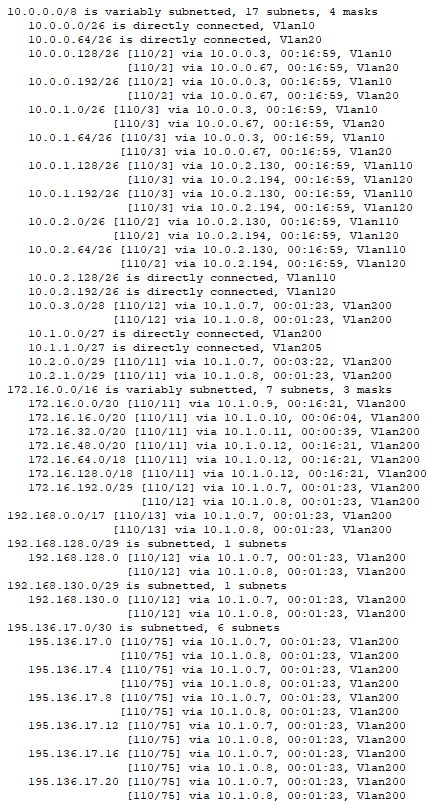
\includegraphics[width=0.5\textwidth]{Imágenes/OSPF Distr.png}
    \caption{OSPF en Switches de Distribución en Hospital Son Espases}
\end{figure}

\section{Validación DHCP}\label{anexo:Pruebadhcp}
A continuación se muestran algunas imágenes que corroboran que el protocolo DHCP está correctamente configurado y asigna direcciones IPs dinámicas a los dispositivos de la red.
\subsection{Dirección IP Dinámica en PC de Recursos Humanos}
\begin{figure}[H]
    \centering
    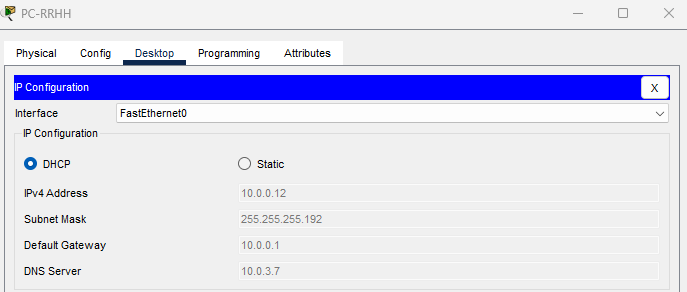
\includegraphics[width=0.5\textwidth]{Imágenes/DHCP-PC-RRHH.png}
    \caption{Dirección IP Dinámica en PC de Recursos Humanos}
\end{figure}
\subsection{Dirección IP Dinámica en PC de Admisión}
\begin{figure}[H]
    \centering
    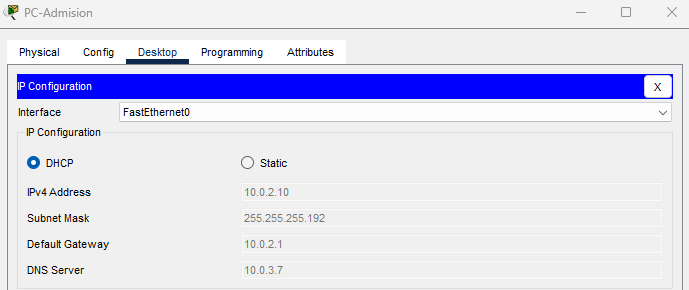
\includegraphics[width=0.5\textwidth]{Imágenes/DHCP-PC-Admision.png}
    \caption{Dirección IP Dinámica en PC de Admisión}
\end{figure}

\section{Validación NAT}
A continuación se muestran las traducciones de direcciones IPs hechas por el servicio NAT, que permiten la conectividad entre los dispositivos internos con Internet y viceversa.
\subsection{Traducción IPs hacia Internet}\label{anexo:haciaInt}
\begin{figure}[H]
    \centering
    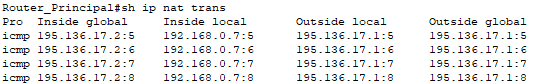
\includegraphics[width=0.5\textwidth]{Imágenes/natHaciaInternet.png}
    \caption{Traducción IPs hacia Internet}
\end{figure}
\subsection{Traducción IPs desde Internet}\label{anexo:desdeInt}
\begin{figure}[H]
    \centering
    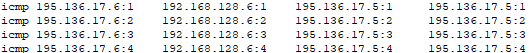
\includegraphics[width=0.5\textwidth]{Imágenes/natdesdeIntenret.png}
    \caption{Traducción IPs desde Internet}
\end{figure}

\section{Validación SSH}\label{anexo:pruebaSSH}
A continuación se muestra la imágen de la consola, donde se ve la conexión realizada mediante SSH a un dispositivo de red del hospital.
\begin{figure}[H]
    \centering
    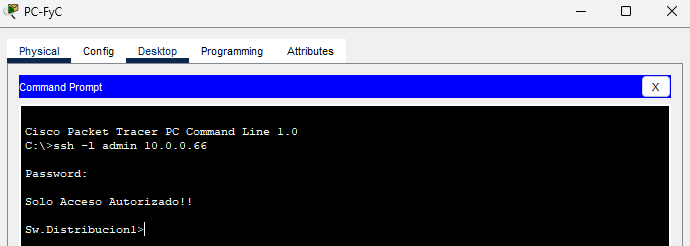
\includegraphics[width=0.5\textwidth]{Imágenes/ssh.png}
    \caption{Conexión Remota mediante SSH a Switch de Distribución 1}
\end{figure}

\section{Validación Autenticación en Dispositivos de Red}\label{anexo:pruebaAutent}
A continuación se muestra la imágen de la consola, donde se ve la autenticación realizada para poder acceder al switch de distribución 2.
\begin{figure}[H]
    \centering
    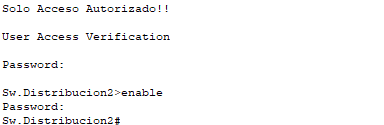
\includegraphics[width=0.5\textwidth]{Imágenes/Autent.png}
    \caption{Autenticación en Switch de Distribución 2}
\end{figure}

\section{Validación VPN IPSec}\label{anexo:pruebavpn}
A continuación se muestra la imágen de la consola, donde se ve la salida dada al insertar el comando "show crypto ipsec sa".
\begin{figure}[H]
    \centering
    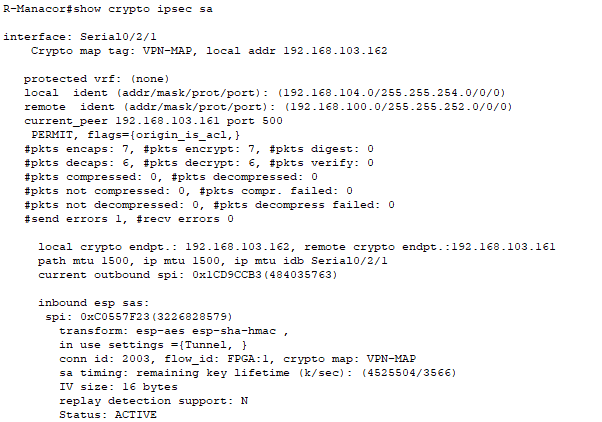
\includegraphics[width=0.5\textwidth]{Imágenes/vpn.png}
    \caption{Salida por consola de show crypto ipsec sa}
\end{figure}

\section{Validación DHCP Snooping}
\subsection{Interfaces en Modo Trusted}\label{anexo:pruebasnoo1}
A continuación se muestra la imágen de la consola, donde se ve la salida dada al insertar el comando "show ip dhcp snooping".
\begin{figure}[H]
    \centering
    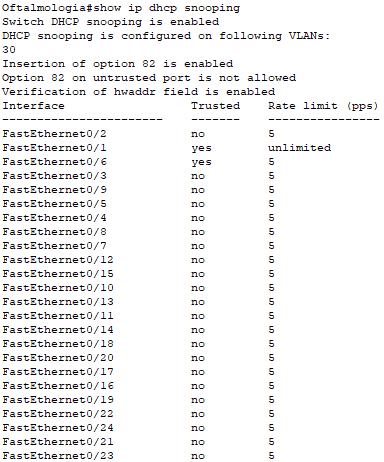
\includegraphics[width=0.5\textwidth]{Imágenes/dhcpsnooping.png}
    \caption{Salida por consola de show ip dhcp snooping}
\end{figure}

\subsection{Tabla de IPs}\label{anexo:pruebasnoo2}
A continuación se muestra la imágen de la consola, donde se ve la salida dada al insertar el comando "show ip dhcp snooping binding".
\begin{figure}[H]
    \centering
    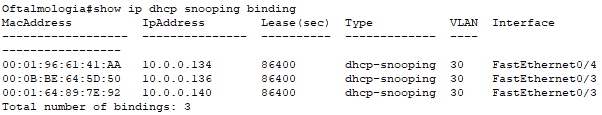
\includegraphics[width=0.5\textwidth]{Imágenes/snooping2.png}
    \caption{Salida por consola de show ip dhcp snooping binding}
\end{figure}

\section{Validación Conectividad}
\subsection{Conectividad Dispositivos Internos con Internet}\label{anexo:pruebaInt-Inter}
A continuación se muestra la imágen de la consola, donde se ve la salida dada al realizar el ping desde un PC de la red interna a la puerta de enlace del ISP 1 (Internet).
\begin{figure}[H]
    \centering
    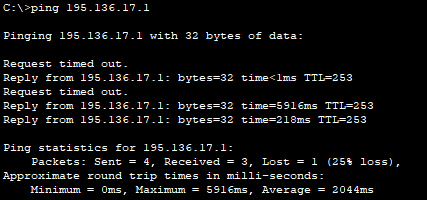
\includegraphics[width=0.5\textwidth]{Imágenes/inv-internet.png}
    \caption{Conectividad Dispositivos Internos con Internet}
\end{figure}
\subsection{Conectividad Dispositivos Invitados con Internet}\label{anexo:pruebaInv-Inter}
A continuación se muestra la imágen de la consola, donde se ve la salida dada al realizar el ping desde el portátil de la red de invitados a la puerta de enlace del ISP 1 (Internet).
\begin{figure}[H]
    \centering
    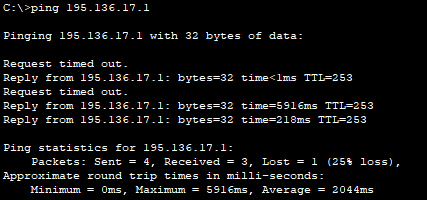
\includegraphics[width=0.5\textwidth]{Imágenes/inv-internet.png}
    \caption{Conectividad Dispositivos Invitados con Internet}
\end{figure}
\subsection{Conectividad Internet con Servidor Web}\label{anexo:pruebaInter-Serv}
A continuación se muestra la imágen de la consola, donde se ve la salida dada al realizar el ping desde la peurta de enlace del ISP 1 (Internet) al servidor web del hospital.
\begin{figure}[H]
    \centering
    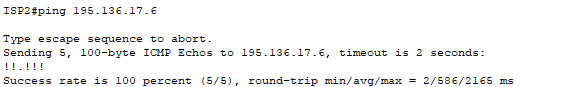
\includegraphics[width=0.5\textwidth]{Imágenes/inter-serv.png}
    \caption{Conectividad Internet con Servidor Web}
\end{figure}

\section{Validación ACLs Bloqueantes}
\subsection{Bloqueo entre Dispositivo Administrativo con Dispositivo IoMT}\label{anexo:blockadmin-iomt}
A continuación se muestra la imágen de la consola, donde se ve la salida dada al realizar el ping entre un dispositivo administrativo con un dispositivo IoMT.
\begin{figure}[H]
    \centering
    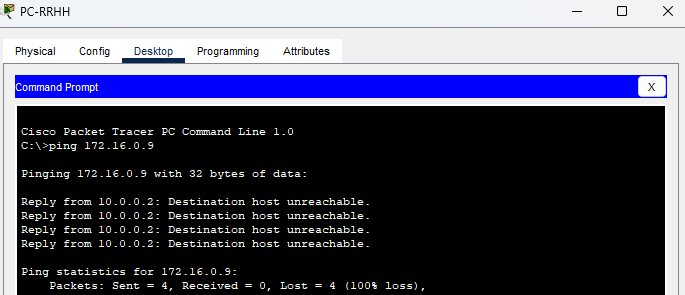
\includegraphics[width=0.5\textwidth]{Imágenes/BlockAdmin-Iomt.png}
    \caption{Bloqueo entre Dispositivo Administrativo con Dispositivo IoMT}
\end{figure}
\subsection{Bloqueo entre Dispositivo Administrativo con Dispositivo Médico}\label{anexo:blockadmin-med}
A continuación se muestra la imágen de la consola, donde se ve la salida dada al realizar el ping entre un dispositivo administrativo con un dispositivo médico.
\begin{figure}[H]
    \centering
    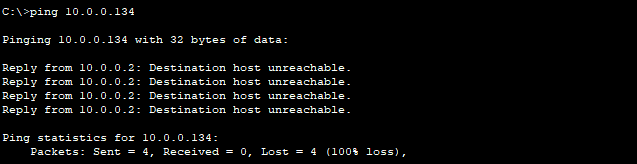
\includegraphics[width=0.5\textwidth]{Imágenes/blockadmin-medico.png}
    \caption{Bloqueo entre Dispositivo Administrativo con Dispositivo Médico}
\end{figure}
\subsection{Bloqueo entre Dispositivo Administrativo con Dispositivo de la UCI}\label{anexo:blockadmin-uci}
A continuación se muestra la imágen de la consola, donde se ve la salida dada al realizar el ping entre un dispositivo administrativo con un dispositivo de la UCI.
\begin{figure}[H]
    \centering
    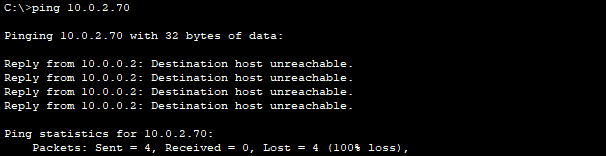
\includegraphics[width=0.5\textwidth]{Imágenes/blockadmin-uci.png}
    \caption{Bloqueo entre Dispositivo Administrativo con Dispositivo de la UCI}
\end{figure}
\subsection{Bloqueo entre Dispositivo Invitado con Dispositivo Interno}\label{anexo:blockinv-int}
A continuación se muestra la imágen de la consola, donde se ve la salida dada al realizar el ping entre un dispositivo invitado con un dispositivo interno.
\begin{figure}[H]
    \centering
    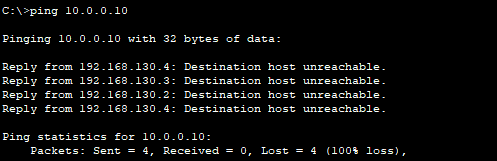
\includegraphics[width=0.5\textwidth]{Imágenes/blockinv-int.png}
    \caption{Bloqueo entre Dispositivo Invitado con Dispositivo Interno}
\end{figure}
\subsection{Bloqueo entre Dispositivo Invitado con Dispositivo IoMT}\label{anexo:blockinv-iomt}
A continuación se muestra la imágen de la consola, donde se ve la salida dada al realizar el ping entre un dispositivo invitado con un dispositivo IoMT.
\begin{figure}[H]
    \centering
    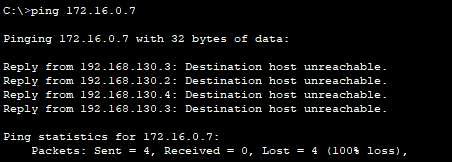
\includegraphics[width=0.5\textwidth]{Imágenes/blockinv-iomt.png}
    \caption{Bloqueo entre Dispositivo Invitado con Dispositivo IoMT}
\end{figure}
\subsection{Bloqueo entre Dispositivo No Autorizado con Servidor de Archivos}\label{anexo:blocknoaut-serv}
A continuación se muestra la imágen de la consola, donde se ve la salida dada al realizar el ping entre un dispositivo invitado con un dispositivo IoMT.
\begin{figure}[H]
    \centering
    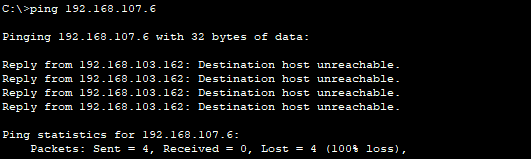
\includegraphics[width=0.5\textwidth]{Imágenes/blocknoaut-serv.png}
    \caption{Bloqueo entre Dispositivo No Autorizado con Servidor de Archivos}
\end{figure}

\section{Validación ACLs Permisivas}
\subsection{Conectividad entre Dispositivo Médico con Dispositivo UCI}\label{anexo:permmed-uci}
A continuación se muestra la imágen de la consola, donde se ve la salida dada al realizar el ping entre un dispositivo médico con un dispositivo de la UCI.
\begin{figure}[H]
    \centering
    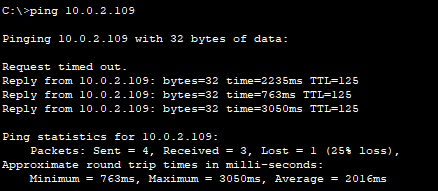
\includegraphics[width=0.5\textwidth]{Imágenes/permmed-uci.png}
    \caption{Conectividad entre Dispositivo Médico con Dispositivo UCI}
\end{figure}
\subsection{Conectividad entre Dispositivo Médico con Dispositivo IoMT Tipo 1}\label{anexo:permmed-tipo1}
A continuación se muestra la imágen de la consola, donde se ve la salida dada al realizar el ping entre un dispositivo médico con un dispositivo IoMT tipo 1.
\begin{figure}[H]
    \centering
    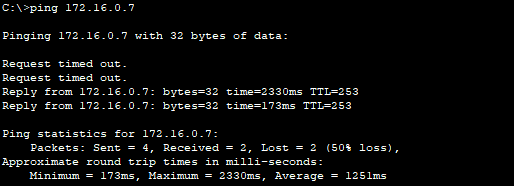
\includegraphics[width=0.5\textwidth]{Imágenes/permmed-tipo1.png}
    \caption{Conectividad entre Dispositivo Médico con Dispositivo IoMT Tipo 1}
\end{figure}
\subsection{Conectividad entre Dispositivo de la UCI con Dispositivo IoMT Tipo 2}\label{anexo:permuci-tipo2}
A continuación se muestra la imágen de la consola, donde se ve la salida dada al realizar el ping entre un dispositivo de la UCI con un dispositivo IoMT tipo 2.
\begin{figure}[H]
    \centering
    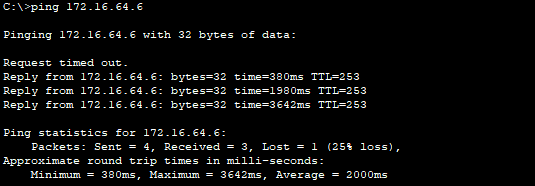
\includegraphics[width=0.5\textwidth]{Imágenes/permuci-tipo2.png}
    \caption{Conectividad entre Dispositivo de la UCI con Dispositivo IoMT Tipo 2}
\end{figure}
\subsection{Conectividad entre Dispositivo Autorizado de la UCI con Dispositivo IoMT Tipo 3}\label{anexo:permuci-tipo3}
A continuación se muestra la imágen de la consola, donde se ve la salida dada al realizar el ping entre el dispositivo autorizado de la UCI con un dispositivo IoMT tipo 3.
\begin{figure}[H]
    \centering
    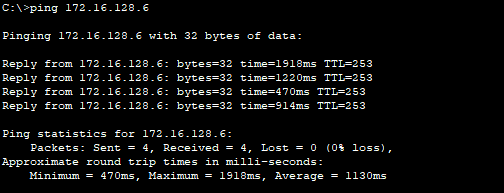
\includegraphics[width=0.5\textwidth]{Imágenes/permuci-tipo3.png}
    \caption{Conectividad entre Dispositivo Autorizado de la UCI con Dispositivo IoMT Tipo 3}
\end{figure}
\subsection{Conectividad PC Autorizado de IT con Servidor de Archivos}\label{anexo:permit-serv}
A continuación se muestra la imágen de la consola, donde se ve la salida dada al realizar el ping entre el PC de IT de Son Espases con el servidor de archivos del hospital de Manacor.
\begin{figure}[H]
    \centering
    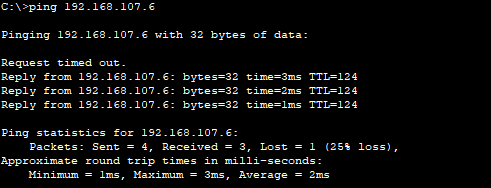
\includegraphics[width=0.5\textwidth]{Imágenes/permaut-serv.png}
    \caption{Conectividad PC Autorizado de IT con Servidor de Archivos}
\end{figure}

\section{Validación HSRP}
\subsection{HSRP en Routers}\label{anexo:pruebahsrprou}
A continuación se muestran las imágenes del estado del HSRP de los tres routers, antes de la caída del router principal y después de la caída del router principal.
\begin{figure}[H]
    \centering
    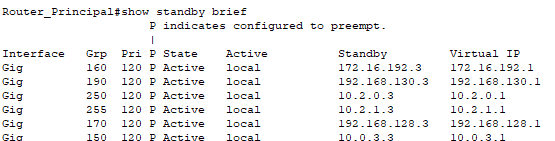
\includegraphics[width=0.5\textwidth]{Imágenes/RprincipalAntes.png}
    \caption{Router Principal Antes}
\end{figure}
\begin{figure}[H]
    \centering
    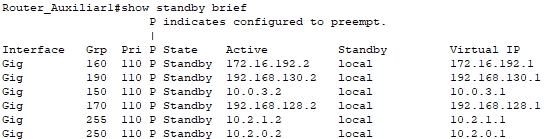
\includegraphics[width=0.5\textwidth]{Imágenes/Rauxiliar1Antes.png}
    \caption{Router Auxiliar 1 Antes}
\end{figure}
\begin{figure}[H]
    \centering
    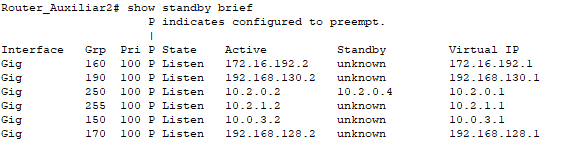
\includegraphics[width=0.5\textwidth]{Imágenes/Rauxiliar2Antes.png}
    \caption{Router Auxiliar 2 Antes}
\end{figure}
\begin{figure}[H]
    \centering
    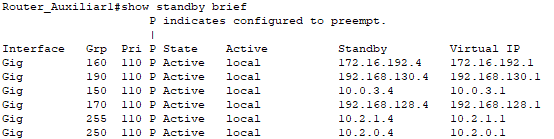
\includegraphics[width=0.5\textwidth]{Imágenes/Rauxiliar1Desp.png}
    \caption{Router Auxiliar 1 Después}
\end{figure}
\begin{figure}[H]
    \centering
    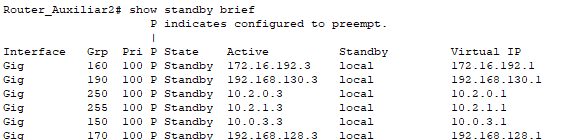
\includegraphics[width=0.5\textwidth]{Imágenes/Rauxiliar2depsues.png}
    \caption{Router Auxiliar 2 Después}
\end{figure}
\subsection{HSRP en Switches}\label{anexo:pruebahsrpsw}
A continuación se muestra las imágenes del estado del HSRP de los dos switches, antes de la caída del switch principal y después de la caída del switch principal.
\begin{figure}[H]
    \centering
    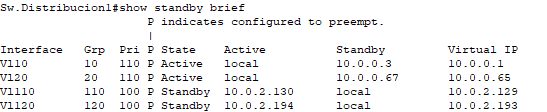
\includegraphics[width=0.5\textwidth]{Imágenes/Sw1Antes.png}
    \caption{Switch Principal Antes}
\end{figure}
\begin{figure}[H]
    \centering
    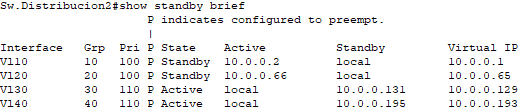
\includegraphics[width=0.5\textwidth]{Imágenes/Sw2Antes.png}
    \caption{Switch Auxiliar Antes}
\end{figure}
\begin{figure}[H]
    \centering
    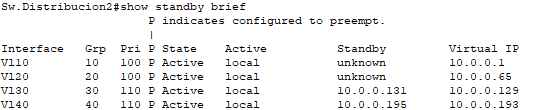
\includegraphics[width=0.5\textwidth]{Imágenes/Sw2Deps.png}
    \caption{Switch Auxiliar Después}
\end{figure}
\section{Validación EtherChannel}\label{anexo:pruebaether}
A continuación se muestra las imágenes del estado del EtherChannel de los dos switches, antes de la caída de un enlace redundante y después de la caída de un enlace redundante.
\begin{figure}[H]
    \centering
    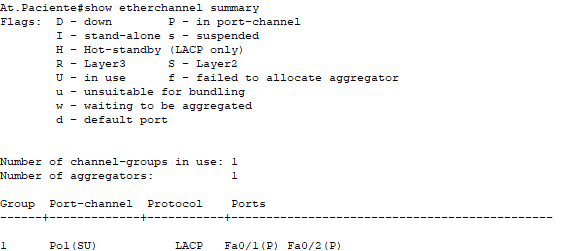
\includegraphics[width=0.5\textwidth]{Imágenes/SwAccAntes.png}
    \caption{Switch Acceso Antes}
\end{figure}
\begin{figure}[H]
    \centering
    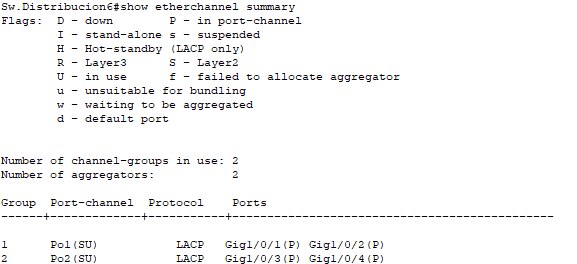
\includegraphics[width=0.5\textwidth]{Imágenes/SwDistrAntes.png}
    \caption{Switch Distribución Antes}
\end{figure}
\begin{figure}[H]
    \centering
    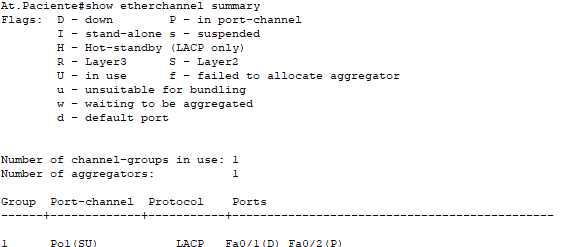
\includegraphics[width=0.5\textwidth]{Imágenes/SwAccDesp.png}
    \caption{Switch Acceso Después}
\end{figure}
\begin{figure}[H]
    \centering
    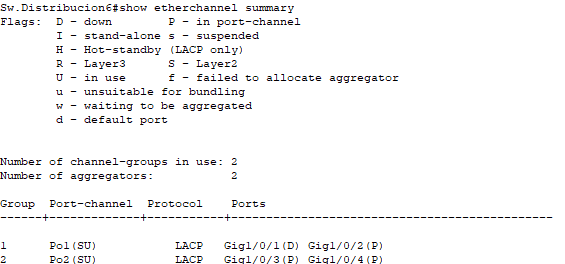
\includegraphics[width=0.5\textwidth]{Imágenes/SwDistrDesp.png}
    \caption{Switch Distribución Después}
\end{figure}
\section{Validación Subred Interconexión}\label{anexo:pruebasubrinter}

\section{Validación OSPF en Red Interconexión entre Hospitales}\label{anexo:ospfinter}
\begin{figure}[H]
    \centering
    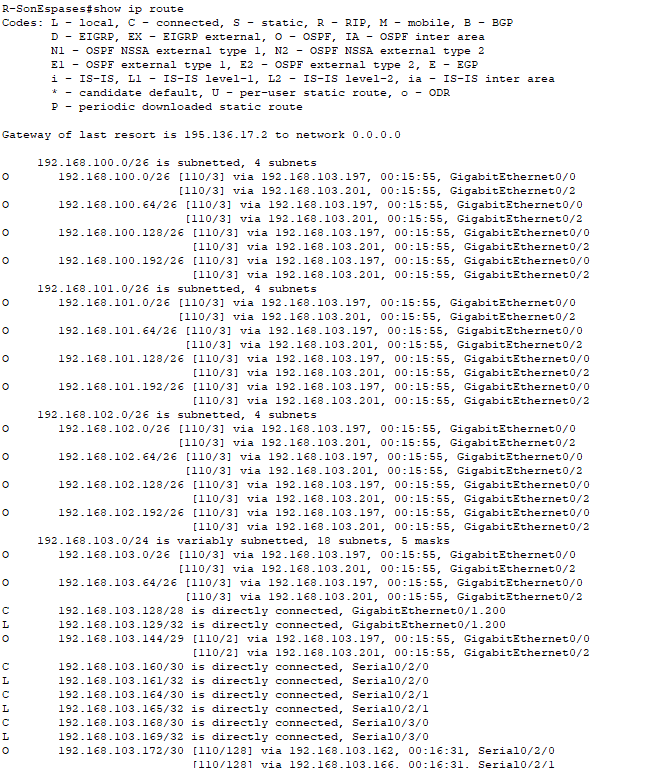
\includegraphics[width=0.5\textwidth]{Imágenes/ospf1.png}
    \caption{Validación OSPF en Red Interconexión entre Hospitales Parte 1}
\end{figure}
\begin{figure}[H]
    \centering
    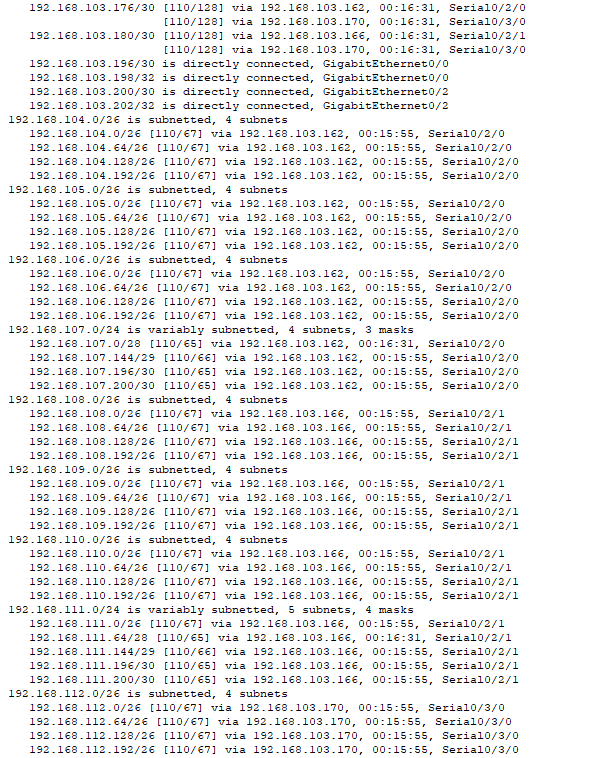
\includegraphics[width=0.5\textwidth]{Imágenes/ospf2.png}
    \caption{Validación OSPF en Red Interconexión entre Hospitales Parte 2}
    \label{fig:interconexion}
\end{figure}
\begin{figure}[H]
    \centering
    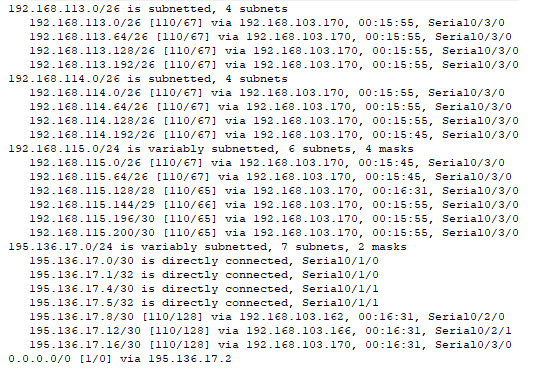
\includegraphics[width=0.5\textwidth]{Imágenes/ospf3.png}
    \caption{Validación OSPF en Red Interconexión entre Hospitales Parte 3}
    \label{fig:interconexion}
\end{figure}

\section{Red Completa del Hospital Son Espases}\label{anexo:redcompletasonespas}
\begin{figure}[H]
    \centering
    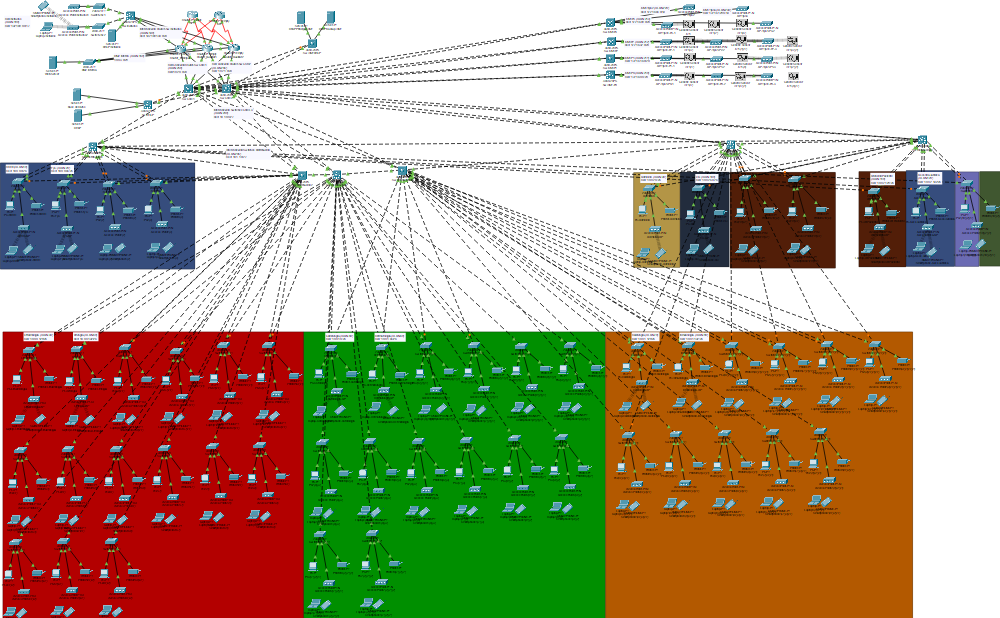
\includegraphics[width=\paperwidth, height=\paperheight, keepaspectratio, angle=270]{Imágenes/RedSonEspases.png}
    \caption{Red Completa del Hospital Son Espases}
    \label{fig:SonEspases}
\end{figure}
\section{Red Completa de Interconexión entre Hospitales}\label{anexo:redcompletahosp}
\begin{figure}[H]
    \centering
    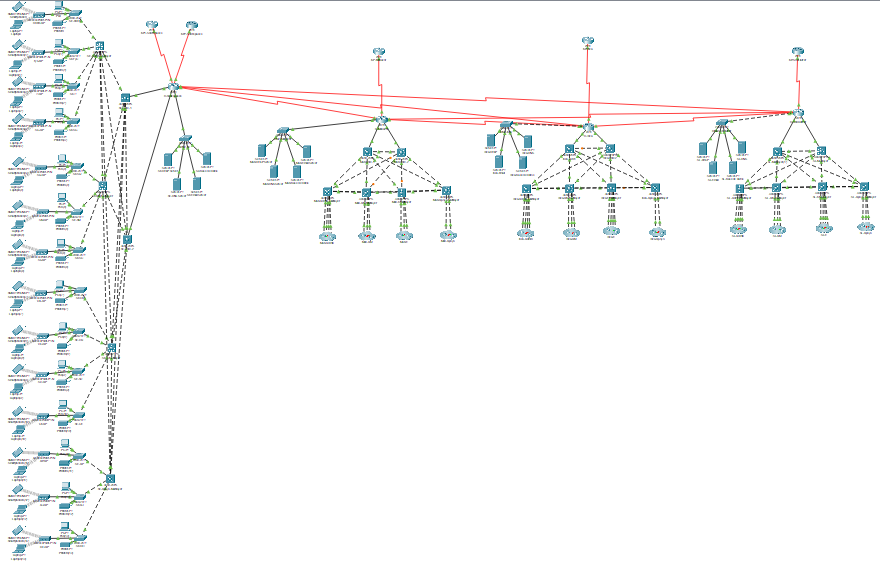
\includegraphics[width=\paperwidth, height=\paperheight, keepaspectratio, angle=270]{Imágenes/redInterocnexion.png}
    \caption{Red Completa de Interconexión entre Hospitales}
    \label{fig:interconexion}
\end{figure}

 

% En aquest cas sols hi ha un fitxer d'annexos,
% però podeu afegir tants \include com calgui. 

%%%%%%% Fi apèndix 

% No toqueu la línia següent 
\backmatter

% La comanda següent defineix l'estil bibliogràfic
\bibliographystyle{IEEEtran}

% La comanda següent defineix el fitxer que
% conté les referències bibliogràfiques.
% En aquest cas és el fitxer Bibliografia.bib
\bibliography{Bibliografia} 

\end{document}